\chapter{Results}
\label{chap:results}


\begin{quote}
      \textit{
            ``Without data, you are just another person with an opinion.'' - W. Edwards Deming
      }
\end{quote}

The last step in the scientific process requires the presentation and objective discussion of empirical findings with good statistical backing. From the problem statements and motivations made in Chapter \ref{chap:introduction}, goals have been defined that broadly include literature studies and a sound empirical process. Thus far, the reader has been provided with a vast scope of background information relevant to the development of the \Acs{BHH}. Chapters \ref{chap:introduction} - \ref{chap:probability} provided the background information, literature studies and existing landscape of research for \acp{ANN}, \index{heuristic}heuristics/\index{optimiser}optimisers, \acp{HH} and probability theory. These elements all share common elements that are required to understand the proposed \Acp{BHH} which was presented in Chapter \ref{chap:bhh}. The details around the empirical process was formally proposed in the methodology as presented in Chapter \ref{chap:methodology}. Finally, the results for the empirical process can be presented and this chapter aims to provide these results.

As a reminder, the empirical process is split into two main experimental groups. These include a behavioural case study and set of comparative studies. This chapter is organised into the same logical pattern. Each of these experimental groups is provided as its own section for detailed analysis and discussion of findings. The remainder of the chapter is structured as follows:

\begin{itemize}
      \item \textbf{Section \ref{sec:results:overview}} provides a brief overview of the general empirical process, high level discussion points and a brief discussion on results interpretation.

      \item \textbf{Section \ref{sec:results:case_study}} provides a detailed analysis of the behaviour of the \Acs{BHH} over a few example runs during training and testing and is meant to introduce the analysis of the \Acs{BHH} from a behavioural characteristic point of view. In this section, focus is put on the learning process itself and to determine what happens during training. It aims to provide insight into ``how'' and ``when'' the \Acs{BHH} learning happens.

      \item \textbf{Section \ref{sec:results:standalone}} provides the first of a series of comparative studies. This section presents the comparative analysis that studies the performance capabilities of the baseline configuration of the \Acs{BHH} to that of standalone/individual low level \index{heuristic}heuristics/\index{optimiser}optimisers. The sections that follow focus on the effect of various parameters on the \Acs{BHH}.

      \item \textbf{Sections \ref{sec:results:heuristic_pool}} - \ref{sec:results:discounted_rewards} capture the results of these empirical processes and focus on the configuration of the \textit{heuristic pool}, the \textit{population size}, \textit{credit assignment strategies}, \textit{reselection} window size, \textit{replay} window size, \textit{reanalysis} window size, \textit{burn in}, \textit{normalisation} and \textit{discounted rewards}, respectfully.

      \item \textbf{Section \ref{sec:results:computational_requirements}} contains a brief discussion on the computational requirements.

      \item \textbf{Section \ref{sec:results:overfitting}} provides a brief discussion on overfitting.

      \item Finally, a summary of the findings is given in \textbf{Section \ref{sec:results:summary}}.
\end{itemize}

\section{Overview}
\label{sec:results:overview}

This section aims to provide a general high level discussion on the outcomes of the empirical process as an introduction to the more detailed discussions to follow. Consider again the goals that have been defined in \ref{chap:introduction}. The empirical component addresses three different angles of analysis:

\begin{enumerate}
      \item Analysing the behaviour of the \Acs{BHH} during training and testing to determine if the the concept works and that the \Acs{BHH} is indeed learning. This component looks at the \Acs{BHH} in isolation and simply evaluates the outcomes of its behaviour over a few example runs and repeats this process for two groups of \Acs{BHH} variants based on \textit{replay} window size.

      \item Comparing the performance capabilities of the \Acs{BHH} to that of well-known low-level \index{heuristic}heuristics that are well researched and understood. This component looks at how the \Acs{BHH} performs given a frame of reference to compare to. Careful consideration of results interpretation must be given here and is discussed in more detail below.

      \item Analysing the effects of various configurations of hyper-parameters for the \Acs{BHH}. This component looks at which parameters have a statistically significant impact on the outcomes of the \Acs{BHH}.
\end{enumerate}

It is important to briefly discuss how results should be interpreted. Traditionally, for typical low-level heuristic training, evaluation of performance is done at a chosen point in time and based on a particular dependent variable. This could be a fixed number of training steps/epochs, early stopped conditions or any other stopping condition. The metric of interest could be a loss value, an accuracy or a rank. Algorithms/heuristics in question are then logically ranked/organised according to their final solution and conclusions are made based on these findings. However, the following arguments suggest an alternative approach for this empirical study:

\begin{itemize}
      \item
            Since there does not exist any research on this specific implementation of \acp{HH} and its application to \acs{FFNN} training, there is no clear point at which it is known that the learning of the \acs{BHH} becomes detrimental to the training process. For example, there exists a currently unknown point during training where the performance bias towards the ``best'' \index{heuristic}heuristic no longer yield improved training or test generalisation outcomes. To cater for this, a fixed maximum number of training epochs have been chosen that empirically have been shown to be sufficient to notice diminishing returns in the outcome. \index{Early stopping}Early stopping was considered, but purposefully not implemented. This is to allow the study of the behaviour and capabilities of the \Acs{BHH} up to and beyond the point of diminishing returns.

      \item
            The training process is to some degree analogous and comparable to a dynamic optimisation problem as previously discussed. This means that the performance of \index{heuristic}heuristics, and thus the \Acs{BHH}, vary at different times during the training process. This hints to the hypothesis that was set in Chapter \ref{chap:introduction} and suggests that there is no single \index{heuristic}heuristic that is always the best \index{heuristic}heuristic to use during all of training. Rather, there exists an applicable, relevant \index{heuristic}heuristic (or combination of \index{heuristic}heuristics) to use at a given point in time during the training process and can change as the process continues. This means the selected \index{heuristic}heuristic at time step $t$ is not necessarily the best heuristic to select at timestamp $t+1$. This argument is further supported by the fact that these experiments are trained on mini-batches, resulting in a lot of noise during training. This noise can cause the \Ac{BHH} to want to "correct" a certain learnt belief. This introduces the same challenges as with \Ac{RL}: Consider delayed rewards, size of rewards, unlearning behaviour that is no longer required, all of which affect the training process throughout and not just at the point of stopping.
\end{itemize}


Based on the points made above, each experimental group is to be evaluated in isolation and has a specific area of focus. For all experimental groups, heuristics are evaluated during \textbf{all} the steps of the training and testing process. For this reason, ranking \index{heuristic}heuristic should not necessarily lead to the conclusion that one heuristic is \textit{better} than another, but rather, that there is a statistically significant difference between the outcomes of heuristics, relative to the entire training and testing process for a given experimental group. The authors suggest further research to include early stopping conditions for the ranking to make entirely sense. However, that does not mean the ranking approach is useless. It still provides a measure of comparison and is indeed indicative of statistically significant outcomes.

The points that have been discussed above have been observed during the empirical process. It is shown in the succeeding sections that the \Acs{BHH} is capable of training \Acp{FFNN} and that it does so relatively well. It is shown that the \Acs{BHH} is generally capable of providing good test generalisations when compared to existing low-level \index{heuristic}heuristics. However, it is shown that the majority of the influence of the \Acs{BHH} occurs during the first few epochs of the training process. Initially uniformly randomised candidate solutions has more room to learn in the initial phases of training in comparison to later phases where learning has become stagnated. It is also shown that this pivotal point of diminishing return is problem specific. Further to this pivotal point, it is shown that the \Acs{BHH} is subject to over-fitting, quite drastically. There are various conclusions that can be made from this point, but the detail is left to the relevant sections to follow.

The following section provides the results and findings for a behavioural case study of the \Acp{BHH} on the iris dataset.


\section{Case Study}
\label{sec:results:case_study}

This section provides a study on the behaviour of the \Acs{BHH} during training and testing. It is important to mention that this experimental group does not necessarily focus on the exact metrics, but rather on the general behaviour of the \Ac{BHH}. This means that statistical analysis and statistical certainty as is not required. Instead, a number of example runs have been executed purely for the intent of analysing behaviour. Furthermore, this behavioural case study is executed on a very small, but well-known toy dataset called \textit{iris}. Iris is not usually considered for full empirical processes due to its size and simplicity. Although there are fourteen other datasets to choose from, iris provides a very simple, relevant and relate-able case study that illustrate the necessary points sufficiently.

Figure \ref{fig:results:case_study:iris:metric_plots} illustrate these runs during training and testing. Take note of the legend as provided in Figure \ref{fig:results:case_study:iris:legend}. There are two variants of the \Acs{BHH} included here, each with three repeated runs, seeded according to run number:

\begin{itemize}
      \item \Acp{BHH} with a very \textbf{short memory}, i.e. replay windows size = 10
      \item \Acp{BHH} with a very \textbf{long memory}, i.e. replay windows size = 250
\end{itemize}

These two groups have been chosen as their parameters have been shown to provide drastically different outcomes from each other during training and forms a good basis for behavioural analysis. For more details on replay window size, see Section \ref{sec:results:replay}.

A breakdown of the run notation as provided in Figure \ref{fig:results:case_study:iris:legend} is then given as follows:

\begin{itemize}
      \item \textbf{iris} - The dataset in question
      \item \textbf{bhh} - The heuristic in question
      \item \textbf{hp:all} - The heuristic pool (hp) in question. ``All'' refers to all the implemented lower-level heuristics including both classical gradient-based heuristics/optimisers as well as meta-heuristics.
      \item \textbf{ps:5} - The population size (ps) in question. In this case, population size = 5.
      \item \textbf{bi:0} - The burn in window size (bi) in question. In this case, burn in window size = 0.
      \item \textbf{rp:10} - The replay window size (rp) in question. In this case, replay window size = 10.
      \item \textbf{rs:10} - The reselection window size (rp) in question. In this case, reselection window size = 10.
      \item \textbf{ra:10} - The reanalysis window size (rp) in question. In this case, reanalysis window size = 10.
      \item \textbf{nm:False} - The normalisation flag (nm) in question. In this case, normalisation is disabled.
      \item \textbf{ct:ibest} - The credit assignment strategy (ct) in question. In this case, the credit assignment strategy used is \textit{ibest}.
      \item \textbf{dr:False} - The discounted rewards flag (dr) in question. In this case, discounted rewards is disabled.
\end{itemize}

From figure \ref{fig:results:case_study:iris:metric_plots} it is shown that the \Acs{BHH} exhibit similar behaviours to that of lower-level heuristics. Figures \ref{fig:results:case_study:iris:train:loss} and \ref{fig:results:case_study:iris:train:accuracy} illustrates a smooth training process, converging to a well-known minimum loss for the iris dataset. In Figures \ref{fig:results:case_study:iris:test:loss} and \ref{fig:results:case_study:iris:test:accuracy} it is shown that the \Acs{BHH} generalised well on the test set. Generalisation improved up to about epoch 10 before overfitting starts occurring. From this, it can be concluded that most of the learning, for this particular dataset, takes place in the first 10 epochs of the training process. From this point onwards, the \Acs{BHH} tries to undo ``bad'' selections made earlier. It is interesting to notice that despite overfitting, the \Acs{BHH} was able to ``correct'' itself to some degree (up to epoch 20), but never really converged back on the minimum it reached up to epoch 10. Early stopping should prohibit this from happening, but this is left for further research.

\begin{figure}[htbp]
      \begin{subfigure}{0.49\textwidth}
            \centering
            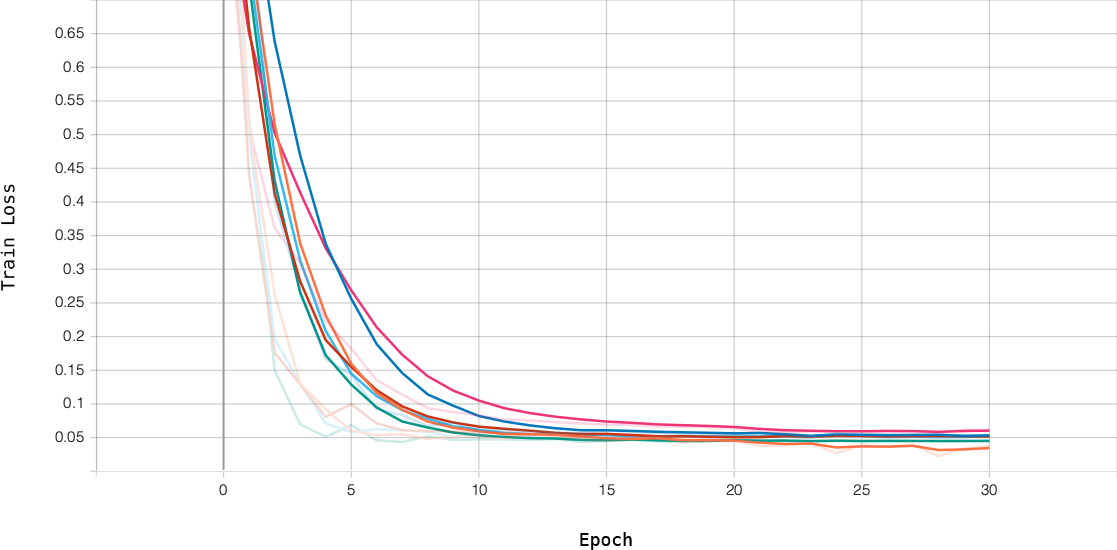
\includegraphics[width=\textwidth]{bhh_case_study/iris/train_loss.png}
            \caption{Train loss}
            \label{fig:results:case_study:iris:train:loss}
      \end{subfigure}
      \begin{subfigure}{0.49\textwidth}
            \centering
            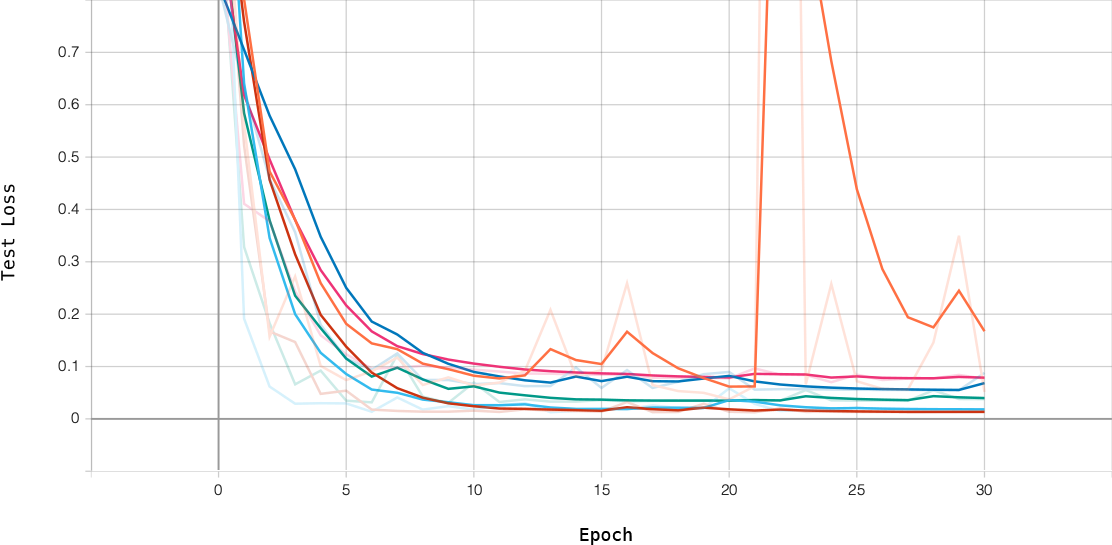
\includegraphics[width=\textwidth]{bhh_case_study/iris/test_loss.png}
            \caption{Test loss}
            \label{fig:results:case_study:iris:test:loss}
      \end{subfigure}
      \par\bigskip
      \begin{subfigure}{0.49\textwidth}
            \centering
            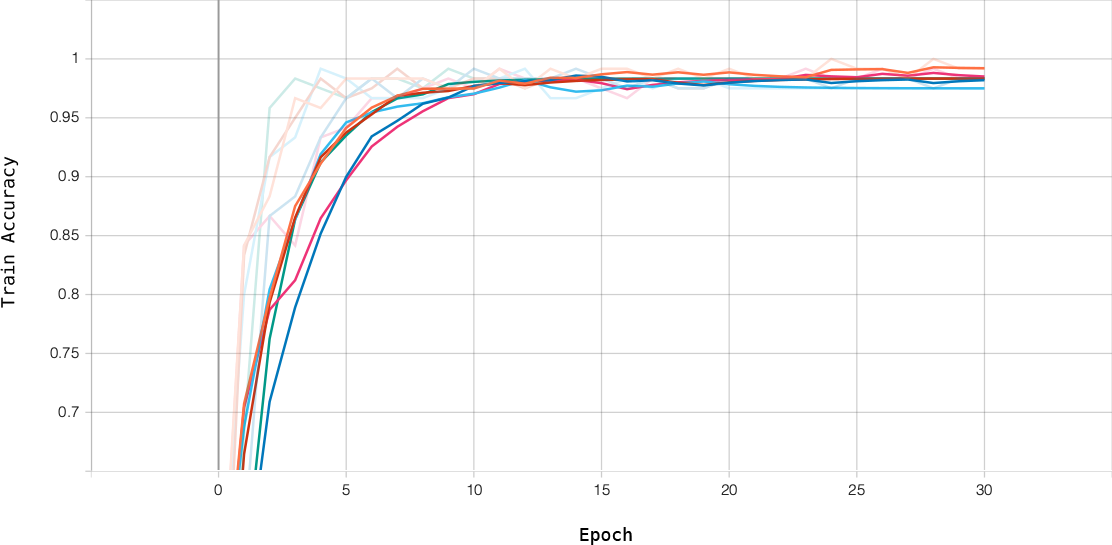
\includegraphics[width=\textwidth]{bhh_case_study/iris/train_accuracy.png}
            \caption{Train accuracy}
            \label{fig:results:case_study:iris:train:accuracy}
      \end{subfigure}
      \begin{subfigure}{0.49\textwidth}
            \centering
            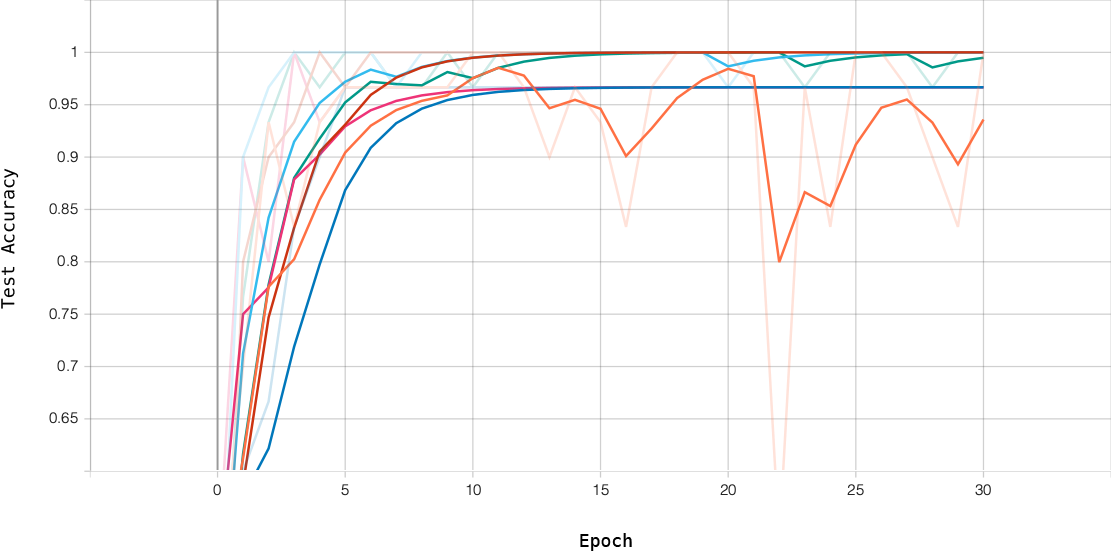
\includegraphics[width=\textwidth]{bhh_case_study/iris/test_accuracy.png}
            \caption{Test accuracy}
            \label{fig:results:case_study:iris:test:accuracy}
      \end{subfigure}
      \par\bigskip
      \begin{subfigure}{\textwidth}
            \centering
            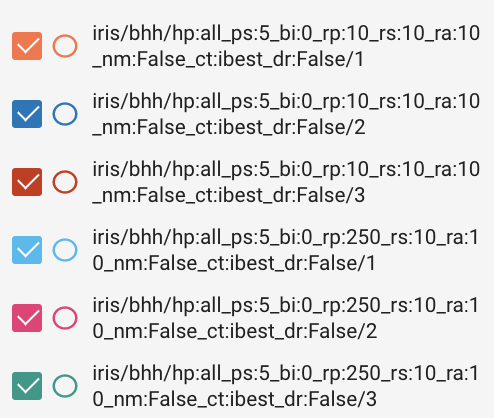
\includegraphics[width=0.35\textwidth]{bhh_case_study/iris/legend.png}
            \caption{Legend}
            \label{fig:results:case_study:iris:legend}
      \end{subfigure}
      \par\bigskip
      \caption{Train and test behaviour of the \Ac{BHH} baseline for different configurations of replay window size}
      \label{fig:results:case_study:iris:metric_plots}
\end{figure}

A high level view of the train and test metric plots is good for drawing high level conclusions, but more detail is required. Figure \ref{fig:results:case_study:iris:alpha} aims to provide more detail as to what is happening during training and plots the value of $\alpha$ during training. Each sub-figure represents the value of $\alpha$ for a particular index, representing a particular \index{heuristic}heuristic. From sub-figures \ref{fig:results:case_study:iris:alpha:0}, \ref{fig:results:case_study:iris:alpha:2} and \ref{fig:results:case_study:iris:alpha:6}, the effect of a larger replay value is clear. Although a more detailed discussed on replay window sizes is left for Section \ref{sec:results:replay}, one can clearly see the accumulation of ``knowledge''/``evidence'' in the concentration parameter $\alpha$. It should be noticeable then from these sub-figures how $\alpha$ changes over time for runs with lower replay window sizes and is indicative of the learning capabilities of the \Ac{BHH}.  From these changes, one can formulate a prediction of which \index{heuristic}heuristics are then likely to be selected in the next steps.

Figures \ref{fig:results:case_study:iris:alpha:5} and \ref{fig:results:case_study:iris:alpha:9} contain a run in orange that shows how the concentration for a particular heuristic (\Acs{Adadelta} and \Acs{DE}) and can change over time. This suggests that the \Acs{BHH} has the ability to dynamically switch between heuristics as the need requires. This concept bears similarities to dynamic optimisation algorithms. It can thus be said that an observation is made that the \Acs{BHH} is able to learn (to some degree) to balance exploration and exploitation by dynamically changing the heuristic of interest at that point in time. Notice that it has not yet been established if the attempt to balance leads to good or bad outcomes. However, this is a still a useful feature of the \Acs{BHH} and warrants further discussion and reasoning. These statements further support the hypothesis that there might not be a no single specific heuristic that is the best heuristic to train the \Acs{FFNN} during the entire training process. In the succeeding sections, it is shown how this statement is further supported as the behaviour of the \Acs{BHH} is shown to be problem-dependent.

A clear distinction between Figures \ref{fig:results:case_study:iris:metric_plots} and \ref{fig:results:case_study:iris:alpha} should be pointed out. Figures \ref{fig:results:case_study:iris:metric_plots} plot metrics for every epoch, while Figure \ref{fig:results:case_study:iris:alpha} plot metrics for every mini-batch iteration. This is a subtle difference in visualisation, but nonetheless important. A more fine-grained visualisation illustrates the learning opportunities better since it is clear that a single step of learning happens on a single mini-batch iteration. This is important to keep in mind for various different sizes of datasets.


\begin{figure}[htbp]
      \begin{subfigure}{0.5\textwidth}
            \centering
            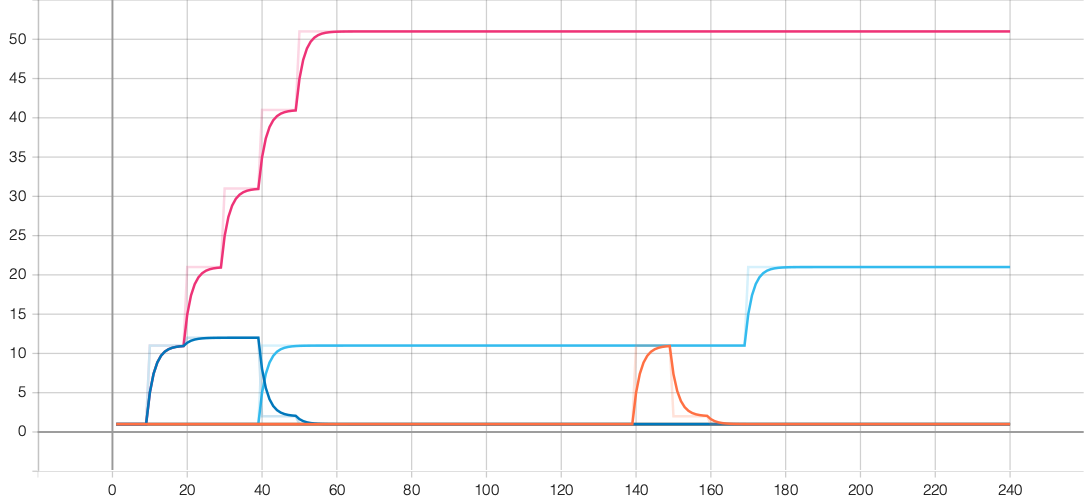
\includegraphics[width=\textwidth]{bhh_case_study/iris/alpha[0].png}
            \caption{$\alpha_{0}$ - \Acs{SGD}}
            \label{fig:results:case_study:iris:alpha:0}
      \end{subfigure}
      \begin{subfigure}{0.5\textwidth}
            \centering
            \includegraphics[width=\textwidth]{bhh_case_study/iris/alpha[1].png}
            \caption{$\alpha_{1}$ - \Acs{Momentum}}
            \label{fig:results:case_study:iris:alpha:1}
      \end{subfigure}
      \par\bigskip
      \begin{subfigure}{0.5\textwidth}
            \centering
            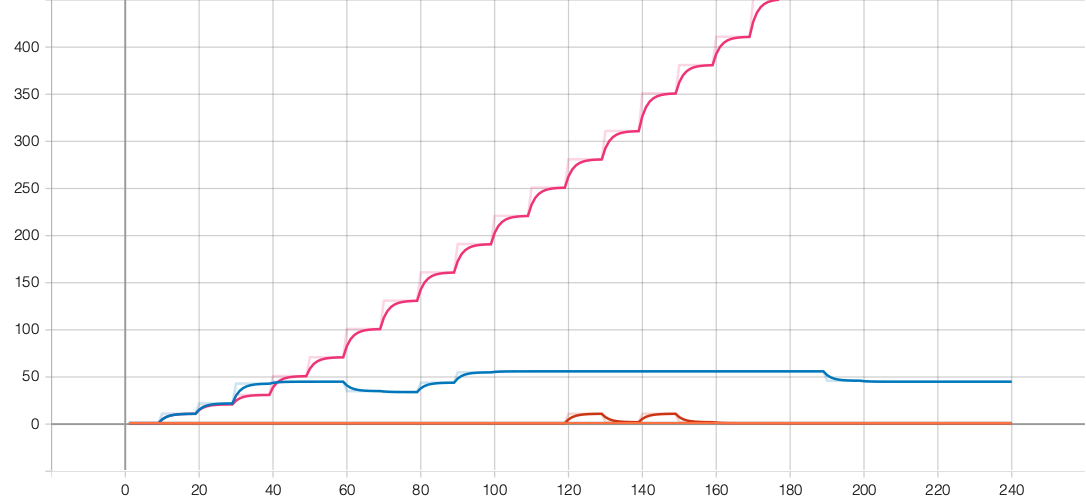
\includegraphics[width=\textwidth]{bhh_case_study/iris/alpha[2].png}
            \caption{$\alpha_{2}$ - \Acs{NAG}}
            \label{fig:results:case_study:iris:alpha:2}
      \end{subfigure}
      \begin{subfigure}{0.5\textwidth}
            \centering
            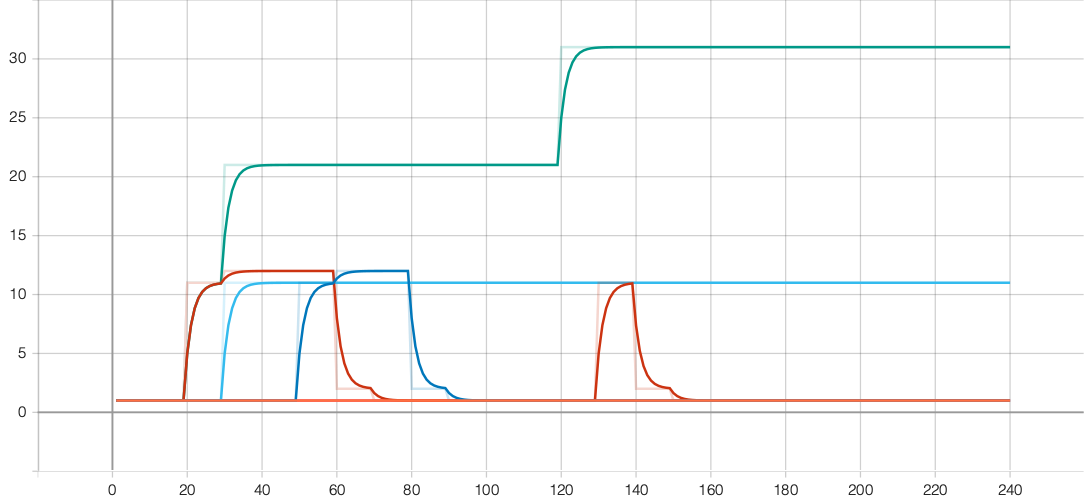
\includegraphics[width=\textwidth]{bhh_case_study/iris/alpha[3].png}
            \caption{$\alpha_{3}$ - \Acs{Adagrad}}
            \label{fig:results:case_study:iris:alpha:3}
      \end{subfigure}
      \par\bigskip
      \begin{subfigure}{0.5\textwidth}
            \centering
            \includegraphics[width=\textwidth]{bhh_case_study/iris/alpha[4].png}
            \caption{$\alpha_{4}$ - \Acs{RMSProp}}
            \label{fig:results:case_study:iris:alpha:4}
      \end{subfigure}
      \begin{subfigure}{0.5\textwidth}
            \centering
            \includegraphics[width=\textwidth]{bhh_case_study/iris/alpha[5].png}
            \caption{$\alpha_{5}$ - \Acs{Adadelta}}
            \label{fig:results:case_study:iris:alpha:5}
      \end{subfigure}
      \par\bigskip
      \begin{subfigure}{0.5\textwidth}
            \centering
            \includegraphics[width=\textwidth]{bhh_case_study/iris/alpha[6].png}
            \caption{$\alpha_{6}$ - \Acs{Adam}}
            \label{fig:results:case_study:iris:alpha:6}
      \end{subfigure}
      \begin{subfigure}{0.5\textwidth}
            \centering
            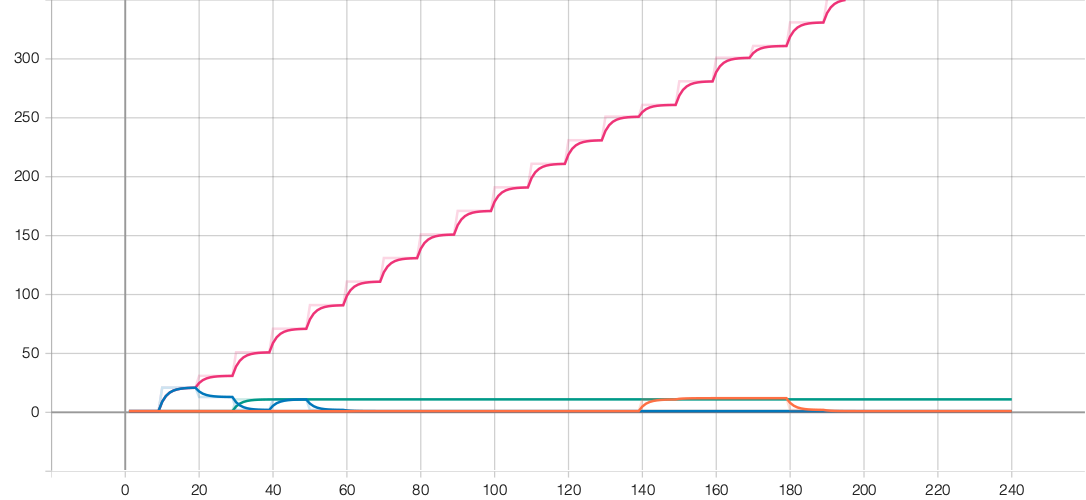
\includegraphics[width=\textwidth]{bhh_case_study/iris/alpha[7].png}
            \caption{$\alpha_{7}$ - \Acs{PSO}}
            \label{fig:results:case_study:iris:alpha:7}
      \end{subfigure}
      \par\bigskip
      \begin{subfigure}{0.5\textwidth}
            \centering
            \includegraphics[width=\textwidth]{bhh_case_study/iris/alpha[8].png}
            \caption{$\alpha_{8}$ - \Acs{GA}}
            \label{fig:results:case_study:iris:alpha:8}
      \end{subfigure}
      \begin{subfigure}{0.5\textwidth}
            \centering
            \includegraphics[width=\textwidth]{bhh_case_study/iris/alpha[9].png}
            \caption{$\alpha_{9}$ - \Acs{DE}}
            \label{fig:results:case_study:iris:alpha:9}
      \end{subfigure}
      \par\bigskip
      \caption{Change in the concentration of $\alpha$ during training for various heuristics}
      \label{fig:results:case_study:iris:alpha}
\end{figure}

Due to the Bayesian nature of the \Acs{BHH}, one can expect the plots from figure \ref{fig:results:case_study:iris:alpha} to drive the plots presented in \ref{fig:results:case_study:iris:p_theta} as these two parameters are related. The parameter $\alpha$ is the concentration parameter for the Dirichlet probability distribution represented by $\theta$. The reader is now urged to consider Figures \ref{fig:results:case_study:iris:alpha:6} and \ref{fig:results:case_study:iris:p_theta:6} together. These two figures illustrate the above mentioned Bayesian concepts well. It should be noted that as $\alpha$ changes, $\theta$ will change. More specifically, the longer the ``memory'' of the \Acs{BHH} the greater the magnitude of $\alpha$ resulting in a sampled selection probability $\theta$ that converges to the ``learnt'' expected selection probability ($E\left[\theta\right]$). The impact of this concept (retained memory) is addressed in Sections \ref{sec:results:replay}.

\begin{figure}[htbp]
      \begin{subfigure}{0.5\textwidth}
            \centering
            \includegraphics[width=\textwidth]{bhh_case_study/iris/theta[0].png}
            \caption{$P(\theta_{0} | \alpha)$ - \Acs{SGD}}
            \label{fig:results:case_study:iris:p_theta:0}
      \end{subfigure}
      \begin{subfigure}{0.5\textwidth}
            \centering
            \includegraphics[width=\textwidth]{bhh_case_study/iris/theta[1].png}
            \caption{$P(\theta_{1} | \alpha)$ - \Acs{Momentum}}
            \label{fig:results:case_study:iris:p_theta:1}
      \end{subfigure}
      \par\medskip
      \begin{subfigure}{0.5\textwidth}
            \centering
            \includegraphics[width=\textwidth]{bhh_case_study/iris/theta[2].png}
            \caption{$P(\theta_{2} | \alpha)$ - \Acs{NAG}}
            \label{fig:results:case_study:iris:p_theta:2}
      \end{subfigure}
      \begin{subfigure}{0.5\textwidth}
            \centering
            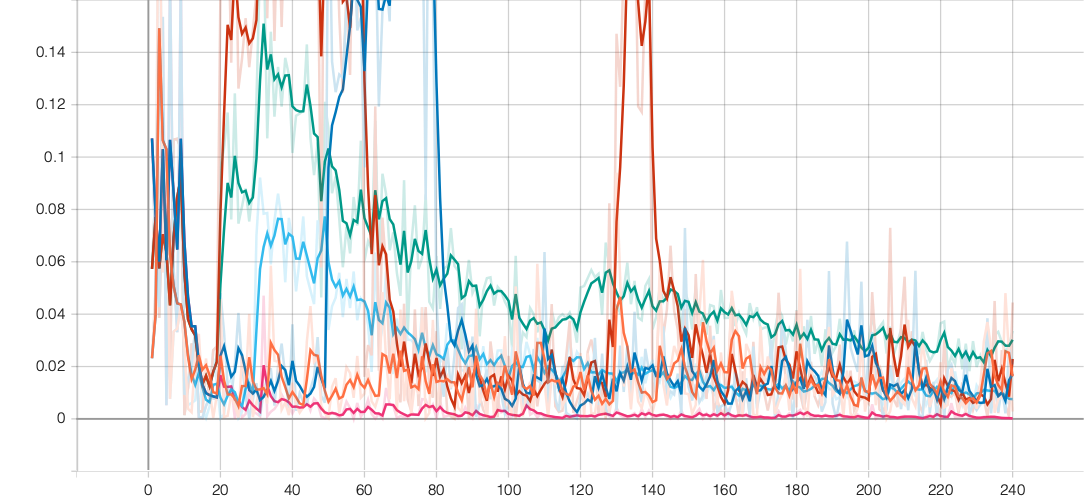
\includegraphics[width=\textwidth]{bhh_case_study/iris/theta[3].png}
            \caption{$P(\theta_{3} | \alpha)$ - \Acs{Adagrad}}
            \label{fig:results:case_study:iris:p_theta:3}
      \end{subfigure}
      \par\medskip
      \begin{subfigure}{0.5\textwidth}
            \centering
            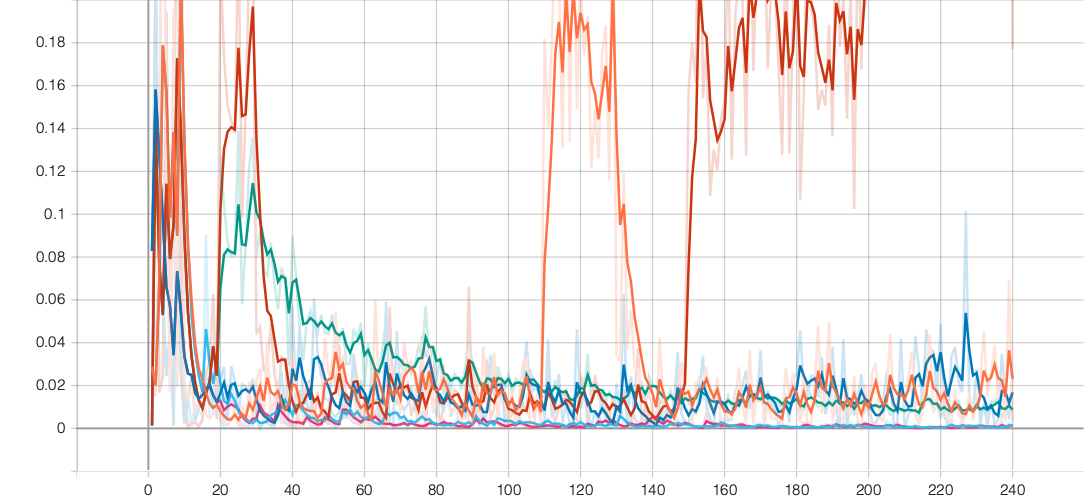
\includegraphics[width=\textwidth]{bhh_case_study/iris/theta[4].png}
            \caption{$P(\theta_{4} | \alpha)$ - \Acs{RMSProp}}
            \label{fig:results:case_study:iris:p_theta:4}
      \end{subfigure}
      \begin{subfigure}{0.5\textwidth}
            \centering
            \includegraphics[width=\textwidth]{bhh_case_study/iris/theta[5].png}
            \caption{$P(\theta_{5} | \alpha)$ - \Acs{Adadelta}}
            \label{fig:results:case_study:iris:p_theta:5}
      \end{subfigure}
      \par\medskip
      \begin{subfigure}{0.5\textwidth}
            \centering
            \includegraphics[width=\textwidth]{bhh_case_study/iris/theta[6].png}
            \caption{$P(\theta_{6} | \alpha)$ - \Acs{Adam}}
            \label{fig:results:case_study:iris:p_theta:6}
      \end{subfigure}
      \begin{subfigure}{0.5\textwidth}
            \centering
            \includegraphics[width=\textwidth]{bhh_case_study/iris/theta[7].png}
            \caption{$P(\theta_{7} | \alpha)$ - \Acs{PSO}}
            \label{fig:results:case_study:iris:p_theta:7}
      \end{subfigure}
      \par\medskip
      \begin{subfigure}{0.5\textwidth}
            \centering
            \includegraphics[width=\textwidth]{bhh_case_study/iris/theta[8].png}
            \caption{$P(\theta_{8} | \alpha)$ - \Acs{GA}}
            \label{fig:results:case_study:iris:p_theta:8}
      \end{subfigure}
      \begin{subfigure}{0.5\textwidth}
            \centering
            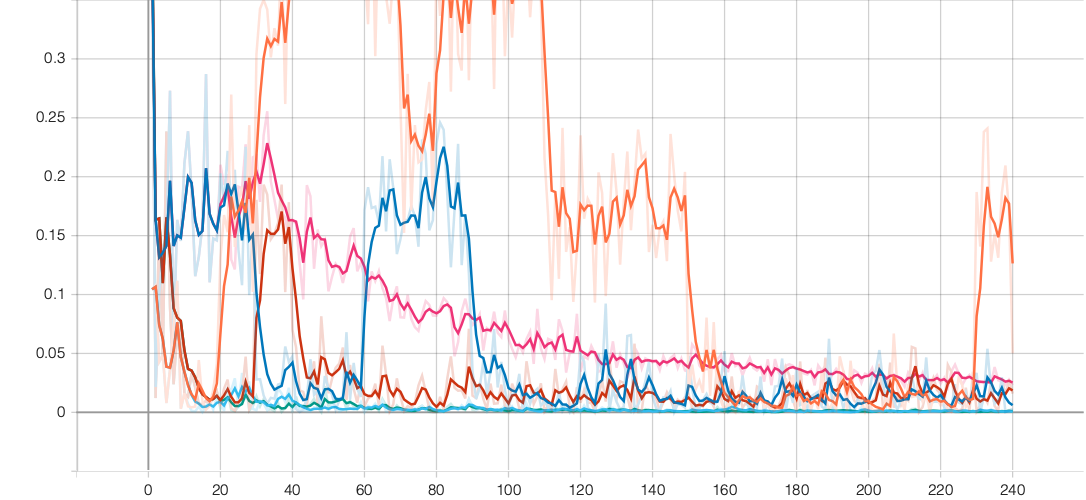
\includegraphics[width=\textwidth]{bhh_case_study/iris/theta[9].png}
            \caption{$P(\theta_{9} | \alpha)$ - \Acs{DE}}
            \label{fig:results:case_study:iris:p_theta:9}
      \end{subfigure}
      \par\medskip
      \caption{Change in the sampled selection probability of $\theta$ during training for various heuristics}
      \label{fig:results:case_study:iris:p_theta}
\end{figure}








Another observation that can be made from Figures \ref{fig:results:case_study:iris:alpha} and \ref{fig:results:case_study:iris:p_theta} is that none of the runs are the same. This is of course due to the stochastic nature of the \Acs{BHH} and the noise caused by using mini-batches. However, it highlights the fact that the learning process for the \Acs{BHH} has to be adaptive from run to run. This is evident in the plots presented in Figure \ref{fig:results:case_study:iris:p_H} as one can see how the \index{heuristic}heuristic selection probability changes over time. This is proof that the \Ac{BHH} is learning something, but it is yet to be established what exactly it is learning. It is said that the \Acs{BHH} updates its \textit{beliefs} (prior knowledge) about which heuristic to select by biasing selection towards \index{heuristic}heuristic performance. It can therefore be concluded that any learning that is done, is done as a result of learning from performance. Since the performance criteria mechanism for the \Ac{BHH}, called the \textit{credit assignment strategy} marks a successful event as one meeting the performance criteria. Although this event is very much a local event, the continuous application of it over all runs means that learning does account for positive learning towards the overall performance goals.




\begin{figure}[htbp]
      \begin{subfigure}{0.5\textwidth}
            \centering
            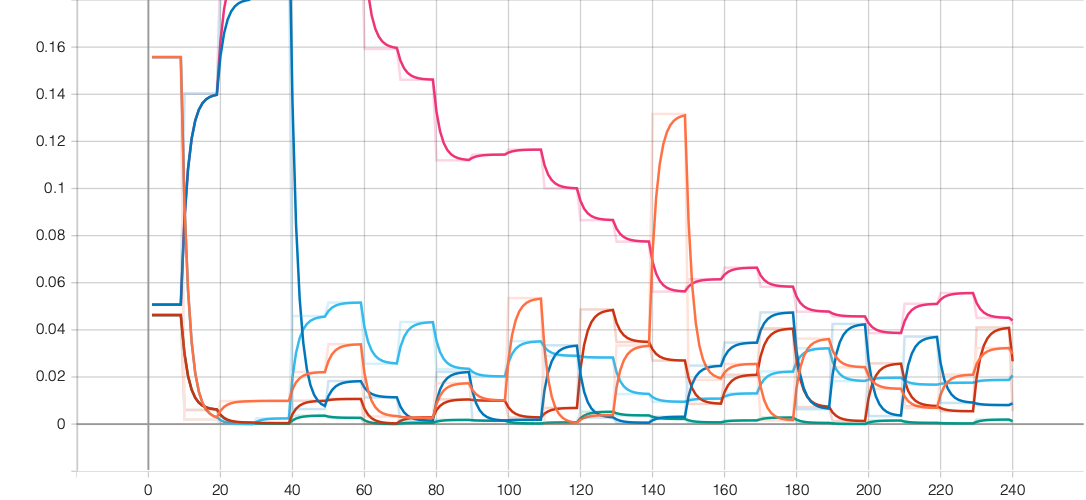
\includegraphics[width=\textwidth]{bhh_case_study/iris/p_H[0].png}
            \caption{$P\left(h_{0} | \theta \right)$ - \Acs{SGD}}
            \label{fig:results:case_study:iris:p_H:0}
      \end{subfigure}
      \begin{subfigure}{0.5\textwidth}
            \centering
            \includegraphics[width=\textwidth]{bhh_case_study/iris/p_H[1].png}
            \caption{$P\left(h_{1} | \theta \right)$ - \Acs{Momentum}}
            \label{fig:results:case_study:iris:p_H:1}
      \end{subfigure}
      \par\medskip
      \begin{subfigure}{0.5\textwidth}
            \centering
            \includegraphics[width=\textwidth]{bhh_case_study/iris/p_H[2].png}
            \caption{$P\left(h_{2} | \theta \right)$ - \Acs{NAG}}
            \label{fig:results:case_study:iris:p_H:2}
      \end{subfigure}
      \begin{subfigure}{0.5\textwidth}
            \centering
            \includegraphics[width=\textwidth]{bhh_case_study/iris/p_H[3].png}
            \caption{$P\left(h_{3} | \theta \right)$ - \Acs{Adagrad}}
            \label{fig:results:case_study:iris:p_H:3}
      \end{subfigure}
      \par\medskip
      \begin{subfigure}{0.5\textwidth}
            \centering
            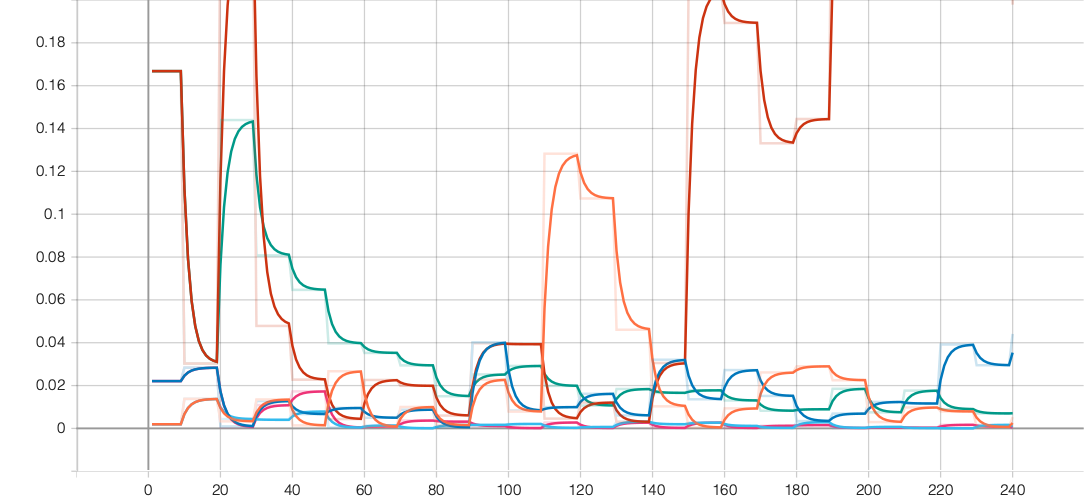
\includegraphics[width=\textwidth]{bhh_case_study/iris/p_H[4].png}
            \caption{$P\left(h_{4} | \theta \right)$ - \Acs{RMSProp}}
            \label{fig:results:case_study:iris:p_H:4}
      \end{subfigure}
      \begin{subfigure}{0.5\textwidth}
            \centering
            \includegraphics[width=\textwidth]{bhh_case_study/iris/p_H[5].png}
            \caption{$P\left(h_{5} | \theta \right)$ - \Acs{Adadelta}}
            \label{fig:results:case_study:iris:p_H:5}
      \end{subfigure}
      \par\medskip
      \begin{subfigure}{0.5\textwidth}
            \centering
            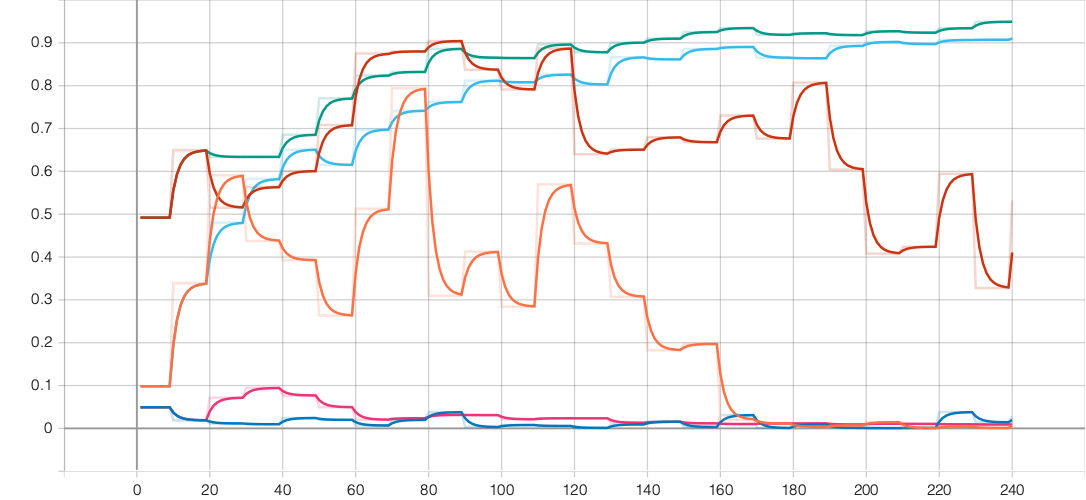
\includegraphics[width=\textwidth]{bhh_case_study/iris/p_H[6].png}
            \caption{$P\left(h_{6} | \theta \right)$ - \Acs{Adam}}
            \label{fig:results:case_study:iris:p_H:6}
      \end{subfigure}
      \begin{subfigure}{0.5\textwidth}
            \centering
            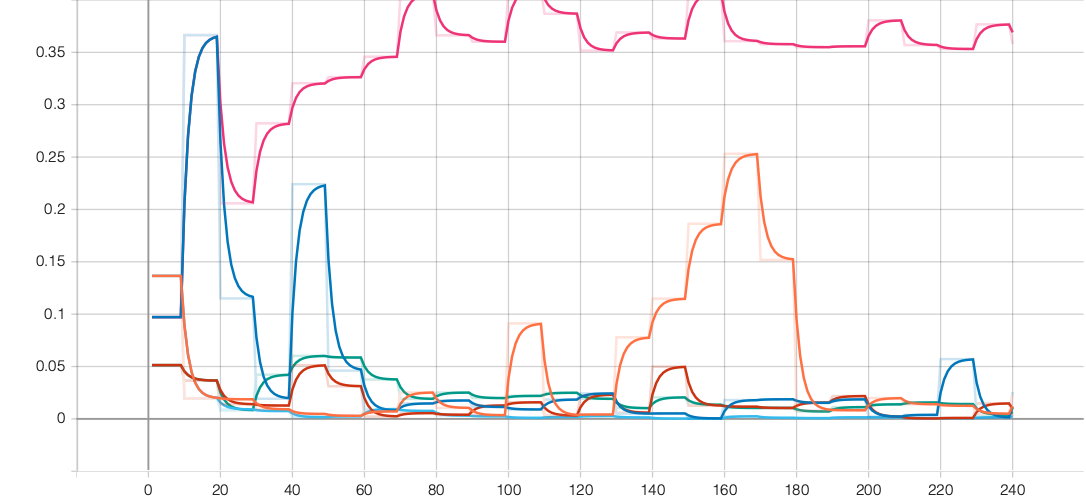
\includegraphics[width=\textwidth]{bhh_case_study/iris/p_H[7].png}
            \caption{$P\left(h_{7} | \theta \right)$ - \Acs{PSO}}
            \label{fig:results:case_study:iris:p_H:7}
      \end{subfigure}
      \par\medskip
      \begin{subfigure}{0.5\textwidth}
            \centering
            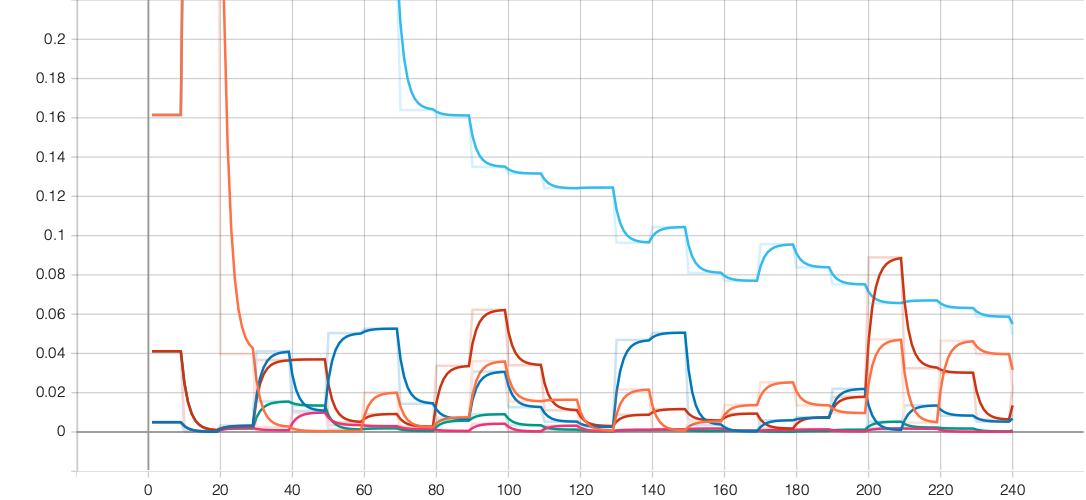
\includegraphics[width=\textwidth]{bhh_case_study/iris/p_H[8].png}
            \caption{$P\left(h_{8} | \theta \right)$ - \Acs{GA}}
            \label{fig:results:case_study:iris:p_H:8}
      \end{subfigure}
      \begin{subfigure}{0.5\textwidth}
            \centering
            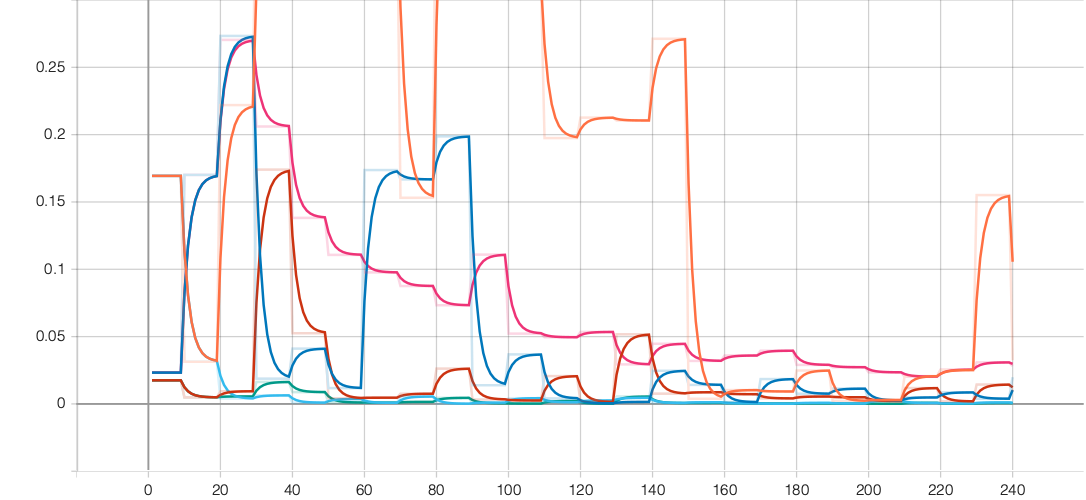
\includegraphics[width=\textwidth]{bhh_case_study/iris/p_H[9].png}
            \caption{$P\left(h_{9} | \theta \right)$ - \Acs{DE}}
            \label{fig:results:case_study:iris:p_H:9}
      \end{subfigure}
      \par\medskip
      \caption{Change in the prior heuristic selection probability $P\left(H\right | \theta )$ as the \Ac{BHH} learns during training}
      \label{fig:results:case_study:iris:p_H}
\end{figure}


Consider now Figure \ref{fig:results:case_study:iris:p_theta:6} again, but this time include a configuration of the \Acs{BHH} where no \index{Bayesian Analysis}Bayesian Analysis takes place, resulting in a purely random \index{heuristic}heuristic selection probability throughout. Such an configuration is given in Figure \ref{fig:results:case_study:iris:no_learn:metrics} below for the sampled \index{heuristic}heuristic selection probability for \Acs{Adam} (gray).

\begin{figure}[htbp]
      \begin{subfigure}{0.5\textwidth}
            \centering
            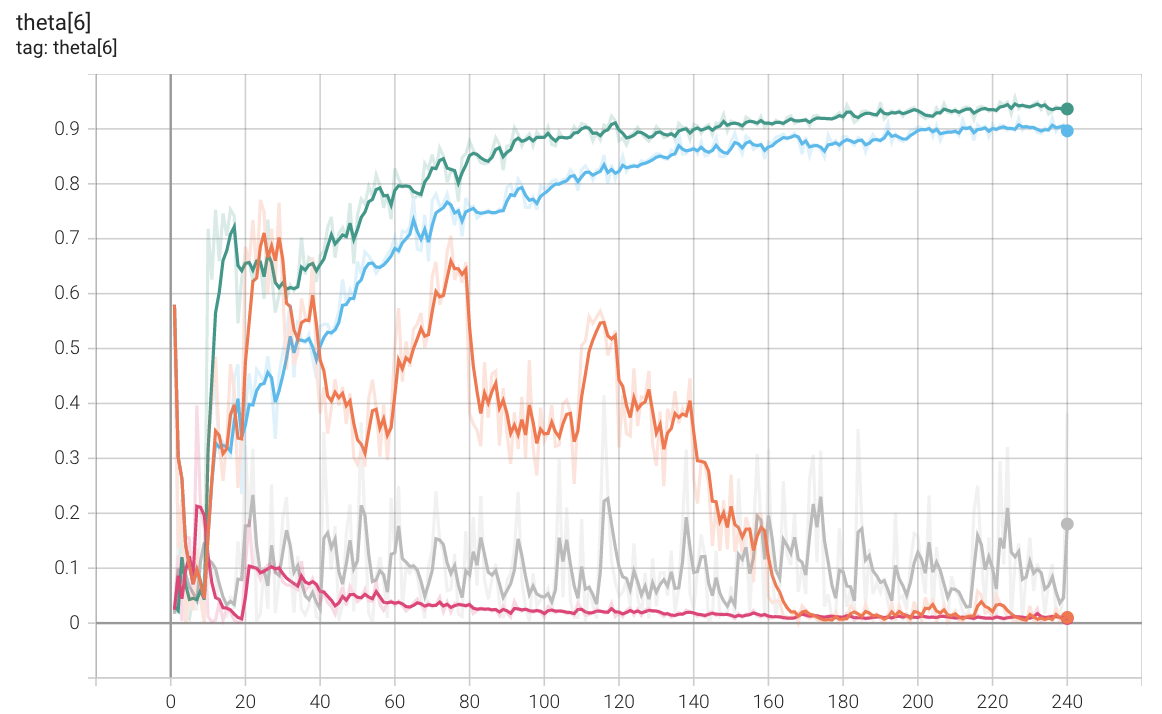
\includegraphics[width=\textwidth]{bhh_case_study/iris/no_learning_theta.png}
            \caption{$P(\theta_{6} | \alpha)$}
            \label{fig:results:case_study:iris:no_learn:p_theta}
      \end{subfigure}
      \begin{subfigure}{0.5\textwidth}
            \centering
            \includegraphics[width=\textwidth]{bhh_case_study/iris/no_learning_test_loss.png}
            \caption{Test loss}
            \label{fig:results:case_study:iris:no_learn:test:loss}
      \end{subfigure}
      \par\bigskip
      \caption{Comparing baseline \Acp{BHH} to that of a \Ac{BHH} with pure random selection.}
      \label{fig:results:case_study:iris:no_learn:metrics}
\end{figure}

One can see that the random configuration (gray) illustrated almost a fixed pattern behaviour, from which we can draw the following conclusions:

\begin{itemize}
      \item Despite a completely random heuristic selection probability, the underlying \Acs{BHH} was still able to learn and perform relatively well. If the ability to learn is then purely based on the \textit{perturbative} components of the \Acs{BHH} it can be concluded that the proxied heuristic step operations are successful.

      \item This shows that the \Acs{BHH} selection mechanism is indeed facilitating a learning process and since \Acs{Adam} is known to perform well on the iris dataset, it can be concluded that the learning process is successful and beneficial to the outcome of the \Acs{BHH}.
\end{itemize}

The statements made above conclude the successful working of the \Acs{BHH}. Both the perturbative element (through proxied heuristic update steps) and the selection mechanism (through Bayesian analysis) is shown to work successfully. Figure \ref{fig:results:case_study:iris:p_HgEC} shows the resulting output of the predictive model for each of the five entities in the heuristic pool. This predicted heuristic selection probability is used to parameterise a new Categorical distribution from which the heuristics are finally sampled and (re)selected.

\begin{figure}[htbp]
      \begin{subfigure}{0.5\textwidth}
            \centering
            \includegraphics[width=\textwidth]{bhh_case_study/iris/p_HgEC[0][6].png}
            \caption{$P\left(h_{6}|e_{0},c_{1}\right)$ - entity 0 + \Acs{Adam} }
            \label{fig:results:case_study:iris:p_HgEC:0:6}
      \end{subfigure}
      \begin{subfigure}{0.5\textwidth}
            \centering
            \includegraphics[width=\textwidth]{bhh_case_study/iris/p_HgEC[1][6].png}
            \caption{$P\left(h_{6}|e_{1},c_{1}\right)$ - entity 1 + \Acs{Adam} }
            \label{fig:results:case_study:iris:p_HgEC:1:6}
      \end{subfigure}
      \par\bigskip
      \begin{subfigure}{0.5\textwidth}
            \centering
            \includegraphics[width=\textwidth]{bhh_case_study/iris/p_HgEC[2][6].png}
            \caption{$P\left(h_{6}|e_{2},c_{1}\right)$ - entity 2 + \Acs{Adam} }
            \label{fig:results:case_study:iris:p_HgEC:2:6}
      \end{subfigure}
      \begin{subfigure}{0.5\textwidth}
            \centering
            \includegraphics[width=\textwidth]{bhh_case_study/iris/p_HgEC[3][6].png}
            \caption{$P\left(h_{6}|e_{3},c_{1}\right)$ - entity 3 + \Acs{Adam} }
            \label{fig:results:case_study:iris:p_HgEC:3:6}
      \end{subfigure}
      \par\bigskip
      \begin{subfigure}{\textwidth}
            \centering
            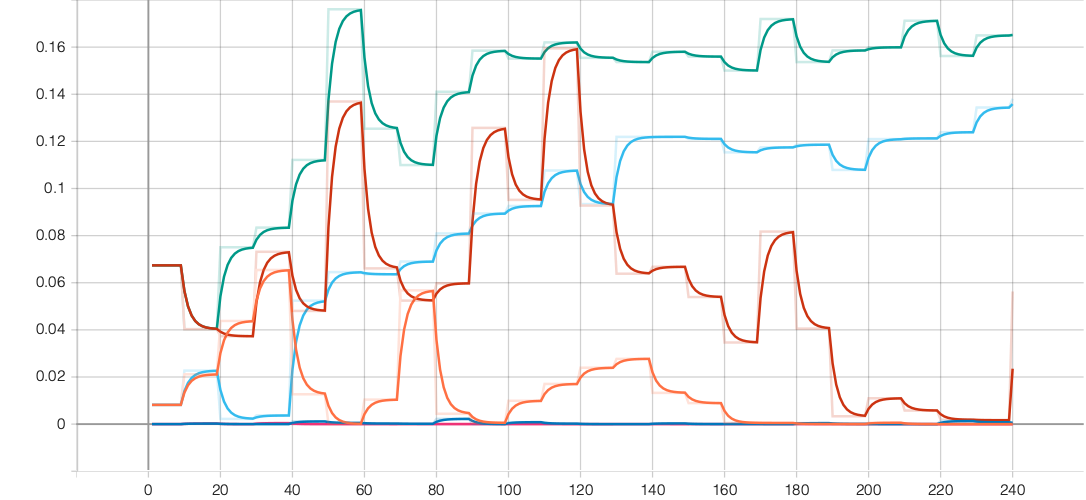
\includegraphics[width=0.5\textwidth]{bhh_case_study/iris/p_HgEC[4][6].png}
            \caption{$P\left(h_{6}|e_{4},c_{1}\right)$ - entity 4 + \Acs{Adam} }
            \label{fig:results:case_study:iris:p_HgEC:4:6}
      \end{subfigure}
      \par\bigskip
      \caption{Change in the realised output of the predictive model $P\left(H|E,C;\theta,\phi,\psi \right)$ showcasing the selection of the \Acs{Adam} optimiser/low-level heuristic as an example}
      \label{fig:results:case_study:iris:p_HgEC}
\end{figure}

Figure \ref{fig:results:case_study:iris:HgEC} show the resulting selected \index{heuristic}heuristic, per entity, over time. From these plots, one can see how convergence on \Acs{Adam} occurs at least at some point during training for the majority of the entities.


\begin{figure}[htbp]
      \begin{subfigure}{0.5\textwidth}
            \centering
            \includegraphics[width=\textwidth]{bhh_case_study/iris/HgEC[0].png}
            \caption{HgEC\lbrack0\rbrack - entity 0}
            \label{fig:results:case_study:iris:HgEC:0}
      \end{subfigure}
      \begin{subfigure}{0.5\textwidth}
            \centering
            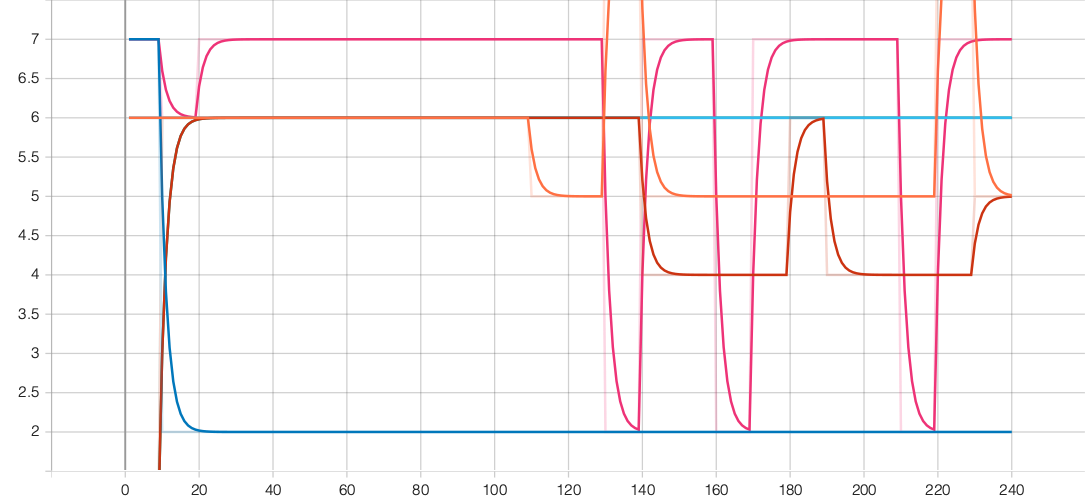
\includegraphics[width=\textwidth]{bhh_case_study/iris/HgEC[1].png}
            \caption{HgEC\lbrack1\rbrack - entity 1}
            \label{fig:results:case_study:iris:HgEC:1}
      \end{subfigure}
      \par\bigskip
      \begin{subfigure}{0.5\textwidth}
            \centering
            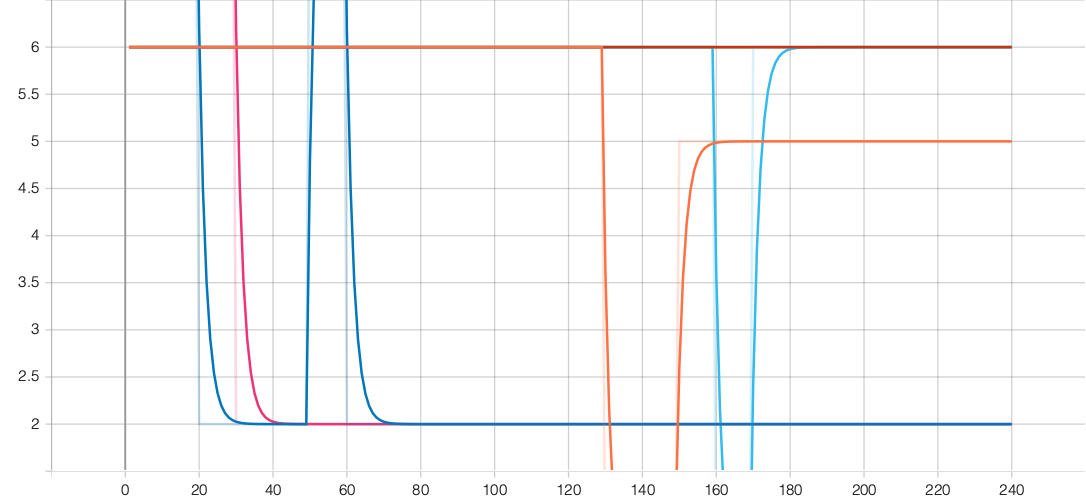
\includegraphics[width=\textwidth]{bhh_case_study/iris/HgEC[2].png}
            \caption{HgEC\lbrack2\rbrack - entity 2}
            \label{fig:results:case_study:iris:HgEC:2}
      \end{subfigure}
      \begin{subfigure}{0.5\textwidth}
            \centering
            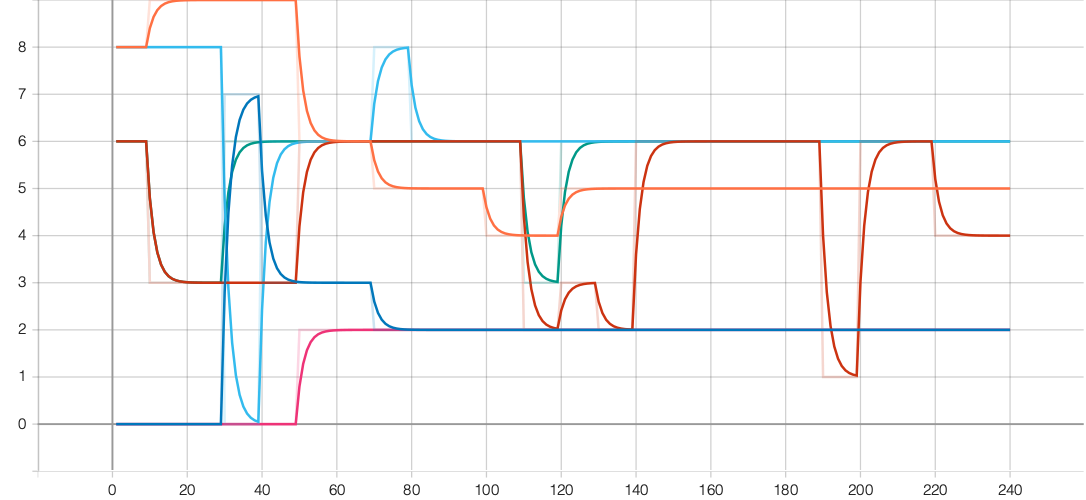
\includegraphics[width=\textwidth]{bhh_case_study/iris/HgEC[3].png}
            \caption{HgEC\lbrack3\rbrack - entity 3}
            \label{fig:results:case_study:iris:HgEC:3}
      \end{subfigure}
      \par\bigskip
      \begin{subfigure}{\textwidth}
            \centering
            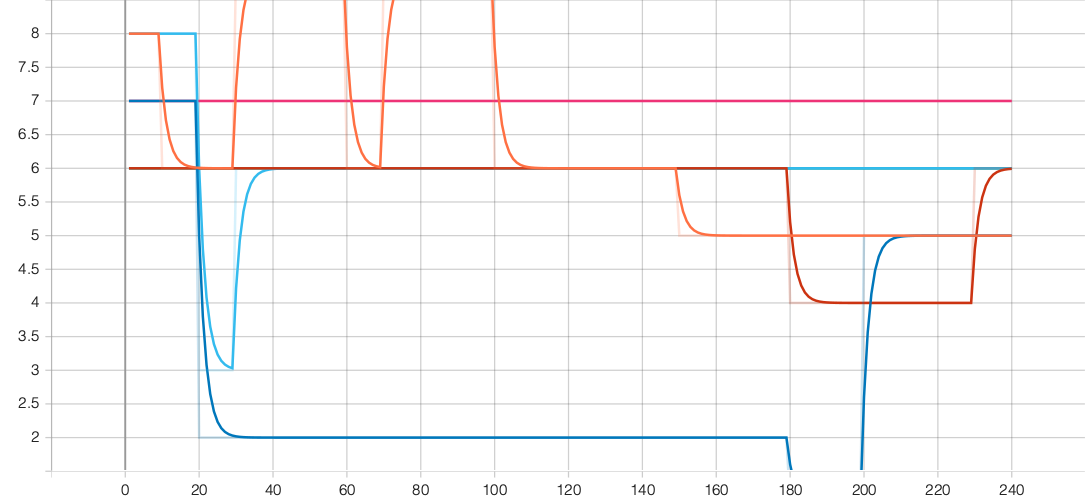
\includegraphics[width=0.5\textwidth]{bhh_case_study/iris/HgEC[4].png}
            \caption{HgEC\lbrack4\rbrack - entity 4}
            \label{fig:results:case_study:iris:HgEC:4}
      \end{subfigure}
      \par\bigskip
      \caption{Change in selected heuristics (HgEC) during training for various entities}
      \label{fig:results:case_study:iris:HgEC}
\end{figure}

Finally, Figure \ref{fig:results:case_study:iris:adam:HgEC} below shows all of the probabilistic components involved in the selection mechanism of the \Ac{BHH}.

\begin{figure}[htbp]
      \begin{subfigure}{0.5\textwidth}
            \centering
            \includegraphics[width=\textwidth]{bhh_case_study/iris/alpha[6].png}
            \caption{$\alpha_{6}$ - \Acs{Adam}}
            \label{fig:results:case_study:iris:adam:alpha:6}
      \end{subfigure}
      \begin{subfigure}{0.5\textwidth}
            \centering
            \includegraphics[width=\textwidth]{bhh_case_study/iris/theta[6].png}
            \caption{$P(\theta_{6} | \alpha)$ - \Acs{Adam}}
            \label{fig:results:case_study:iris:adam:p_theta:6}
      \end{subfigure}
      \par\bigskip
      \begin{subfigure}{0.5\textwidth}
            \centering
            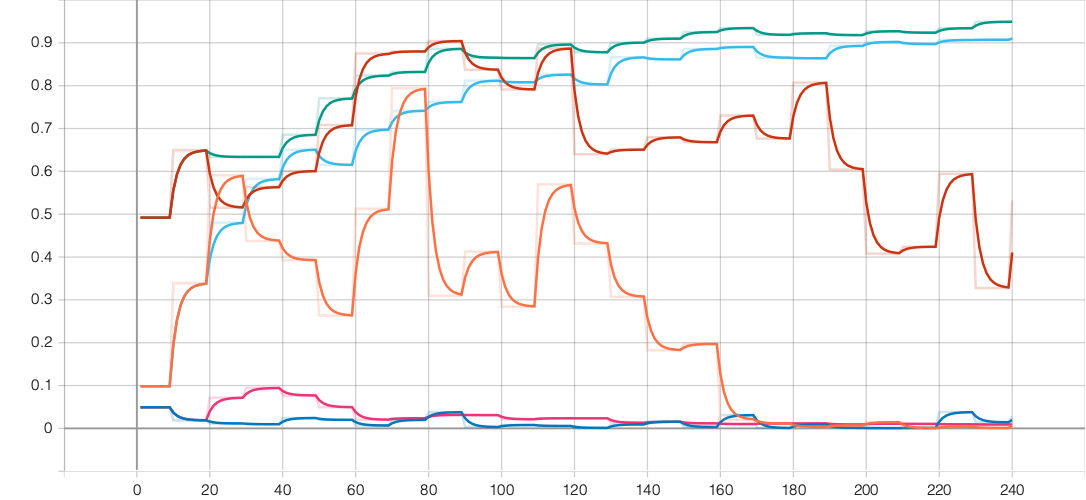
\includegraphics[width=\textwidth]{bhh_case_study/iris/p_H[6].png}
            \caption{$P\left(h_{6} | \theta \right)$ - \Acs{Adam}}
            \label{fig:results:case_study:iris:adam:p_H:6}
      \end{subfigure}
      \begin{subfigure}{0.5\textwidth}
            \centering
            \includegraphics[width=\textwidth]{bhh_case_study/iris/p_HgEC[1][6].png}
            \caption{$P\left(h_{6}|e_{1},c_{1}\right)$ - entity 1 + \Acs{Adam} }
            \label{fig:results:case_study:iris:adam:p_HgEC:1:6}
      \end{subfigure}
      \par\bigskip
      \begin{subfigure}{\textwidth}
            \centering
            \includegraphics[width=0.5\textwidth]{bhh_case_study/iris/HgEC[1].png}
            \caption{HgEC\lbrack1\rbrack - entity 1}
            \label{fig:results:case_study:iris:adam:HgEC:1}
      \end{subfigure}
      \par\bigskip
      \caption{An illustration that shows the effects of learning as for \Acs{Adam}}
      \label{fig:results:case_study:iris:adam:HgEC}
\end{figure}


The behaviour of the \Ac{BHH} has been studied and it is found to be successful in its intent to learn which \index{heuristic}heuristics to use throughout the training process. It has also been shown that the training of the \acp{FFNN} with \Acp{BHH} is done by means of a \index{heuristic}heuristic selection mechanism and proxied \index{heuristic}heuristic update steps, both which have been shown to attribute to the successful training of the \acp{FFNN}.

Although these observations are good, these are still high level and not based on any statistical data. It is purely based on observation over a few runs. The following section aims to provide the first set of conclusions based on a statistically certain comparison of the \Ac{BHH}'s performance to that of standalone low-level \index{heuristic}heuristics.


\section{Standalone vs BHH Baseline}
\label{sec:results:standalone}

This section provides the empirical results of the experiment group that compare the performance of the \Ac{BHH} to that of well-known, standalone, low-level heuristics. Table \ref{tab:results:standalone:metrics} below shows the count, average and standard deviation of the ranks achieved by die various heuristics for all timestamps, across all datasets. Furthermore, the table orders the \index{heuristic}heuristics by a normalised overall rank.

\begin{table}[htbp]
      \centering
      \caption{Empirical results showcasing rank statistics for different standalone \index{heuristic}heuristics compared to the baseline \acs{BHH} across multiple datasets}
      \label{tab:results:standalone:metrics}%
      \par\bigskip
      \resizebox{\textwidth}{!}{
            \begin{tabular}{rcccccccccccc}
                  \textbf{step}                      & \multicolumn{1}{l}{\textbf{(All)}}     &                                                                                    &                                                                           &                                                                           &                                                                           &                                               &                                             &                                                &                                                &                                                &                                                &                                                \\
                  \cmidrule{1-2}                     &                                        &                                                                                    &                                                                           &                                                                           &                                                                           &                                               &                                             &                                                &                                                &                                                &                                                &                                                \\
                                                     &                                        & \multicolumn{1}{l}{\textbf{heuristic}}                                             &                                                                           &                                                                           &                                                                           &                                               &                                             &                                                &                                                &                                                &                                                &                                                \\
                  \cmidrule{3-3}    \textbf{dataset} & \multicolumn{1}{l}{\textbf{statistic}} & \textbf{adagrad}                                                                   & \textbf{adam}                                                             & \textbf{nag}                                                              & \textbf{rmsprop}                                                          & \textbf{bhh}                                  & \textbf{adadelta}                           & \textbf{ga}                                    & \textbf{sgd}                                   & \textbf{pso}                                   & \textbf{momentum}                              & \textbf{de}                                    \\
                  \midrule
                  abalone                            & count                                  & 930                                                                                & 930                                                                       & 930                                                                       & 930                                                                       & 930                                           & 930                                         & 930                                            & 930                                            & 930                                            & 930                                            & 930                                            \\
                                                     & avg                                    & \cellcolor[rgb]{ .776,  .937,  .808}\textcolor[rgb]{ 0,  .38,  0}{2.0323}          & 2.2086                                                                    & 3.8108                                                                    & 4.0849                                                                    & 5.1430                                        & 4.7151                                      & 9.1839                                         & 6.9043                                         & 9.3914                                         & 7.9441                                         & 10.5817                                        \\
                                                     & std                                    & 1.3436                                                                             & 1.5671                                                                    & 1.2760                                                                    & 2.2093                                                                    & 1.9327                                        & 1.1671                                      & 0.9030                                         & 0.7740                                         & 1.5268                                         & 0.9717                                         & 1.1291                                         \\
                  adult                              & count                                  & 930                                                                                & 930                                                                       & 930                                                                       & 930                                                                       & 930                                           & 930                                         & 930                                            & 930                                            & 930                                            & 930                                            & 930                                            \\
                                                     & avg                                    & 5.1570                                                                             & 6.3559                                                                    & \cellcolor[rgb]{ .776,  .937,  .808}\textcolor[rgb]{ 0,  .38,  0}{1.4914} & 5.6968                                                                    & 10.1710                                       & 2.4720                                      & 7.7688                                         & 2.8237                                         & 9.6043                                         & 3.6688                                         & 9.0140                                         \\
                                                     & std                                    & 1.2838                                                                             & 1.4823                                                                    & 0.6870                                                                    & 1.4006                                                                    & 2.2688                                        & 1.2974                                      & 1.3461                                         & 1.1988                                         & 1.6718                                         & 1.3834                                         & 1.5614                                         \\
                  air\_quality                       & count                                  & 930                                                                                & 930                                                                       & 930                                                                       & 930                                                                       & 930                                           & 930                                         & 930                                            & 930                                            & 930                                            & 930                                            & 930                                            \\
                                                     & avg                                    & 3.0688                                                                             & 4.4849                                                                    & 3.2527                                                                    & \cellcolor[rgb]{ .776,  .937,  .808}\textcolor[rgb]{ 0,  .38,  0}{2.9269} & 5.4989                                        & 4.4204                                      & 6.3785                                         & 8.7548                                         & 8.1151                                         & 9.8301                                         & 9.2688                                         \\
                                                     & std                                    & 1.8148                                                                             & 2.0087                                                                    & 1.7266                                                                    & 2.0466                                                                    & 2.5018                                        & 2.5575                                      & 1.7707                                         & 1.4074                                         & 1.9775                                         & 1.3046                                         & 1.9578                                         \\
                  bank                               & count                                  & 930                                                                                & 930                                                                       & 930                                                                       & 930                                                                       & 930                                           & 930                                         & 930                                            & 930                                            & 930                                            & 930                                            & 930                                            \\
                                                     & avg                                    & 2.4161                                                                             & \cellcolor[rgb]{ .776,  .937,  .808}\textcolor[rgb]{ 0,  .38,  0}{1.9882} & 3.8516                                                                    & 3.1591                                                                    & 5.4688                                        & 5.0108                                      & 9.0505                                         & 7.2301                                         & 9.9043                                         & 7.3892                                         & 10.5312                                        \\
                                                     & std                                    & 1.3873                                                                             & 1.3985                                                                    & 1.4056                                                                    & 1.8653                                                                    & 1.7489                                        & 0.9864                                      & 0.9955                                         & 0.9144                                         & 1.2374                                         & 0.8907                                         & 1.0445                                         \\
                  bike                               & count                                  & 930                                                                                & 930                                                                       & 930                                                                       & 930                                                                       & 930                                           & 930                                         & 930                                            & 930                                            & 930                                            & 930                                            & 930                                            \\
                                                     & avg                                    & \cellcolor[rgb]{ .776,  .937,  .808}\textcolor[rgb]{ 0,  .38,  0}{1.6710}          & 3.2559                                                                    & 5.4247                                                                    & 5.4140                                                                    & 3.5903                                        & 4.3774                                      & 7.2591                                         & 8.3656                                         & 7.4000                                         & 8.7441                                         & 10.4978                                        \\
                                                     & std                                    & 1.1854                                                                             & 3.2580                                                                    & 0.9310                                                                    & 3.7231                                                                    & 1.0534                                        & 1.0684                                      & 1.0992                                         & 1.3163                                         & 1.6037                                         & 1.2745                                         & 1.2717                                         \\
                  car                                & count                                  & 930                                                                                & 930                                                                       & 930                                                                       & 930                                                                       & 930                                           & 930                                         & 930                                            & 930                                            & 930                                            & 930                                            & 930                                            \\
                                                     & avg                                    & 3.8591                                                                             & \cellcolor[rgb]{ .776,  .937,  .808}\textcolor[rgb]{ 0,  .38,  0}{1.5022} & 5.0839                                                                    & 2.0946                                                                    & 2.9720                                        & 6.5903                                      & 8.9301                                         & 8.4108                                         & 7.0118                                         & 9.0731                                         & 10.4720                                        \\
                                                     & std                                    & 0.8054                                                                             & 1.1602                                                                    & 0.6925                                                                    & 1.1095                                                                    & 1.0151                                        & 1.4439                                      & 1.2877                                         & 1.2333                                         & 1.2970                                         & 1.1743                                         & 1.2916                                         \\
                  diabetic                           & count                                  & 930                                                                                & 930                                                                       & 930                                                                       & 930                                                                       & 930                                           & 930                                         & 930                                            & 930                                            & 930                                            & 930                                            & 930                                            \\
                                                     & avg                                    & 2.6129                                                                             & 6.0634                                                                    & \cellcolor[rgb]{ .776,  .937,  .808}\textcolor[rgb]{ 0,  .38,  0}{1.7473} & 5.8387                                                                    & 7.9452                                        & 2.5129                                      & 9.2409                                         & 5.1968                                         & 8.7527                                         & 5.5516                                         & 10.5376                                        \\
                                                     & std                                    & 1.3914                                                                             & 1.6944                                                                    & 1.2492                                                                    & 2.0128                                                                    & 2.4141                                        & 1.3843                                      & 1.2206                                         & 1.2711                                         & 0.9424                                         & 1.3025                                         & 1.0607                                         \\
                  fish\_toxicity                     & count                                  & 930                                                                                & 930                                                                       & 930                                                                       & 930                                                                       & 930                                           & 930                                         & 930                                            & 930                                            & 930                                            & 930                                            & 930                                            \\
                                                     & avg                                    & 3.6032                                                                             & 3.0742                                                                    & 4.8742                                                                    & \cellcolor[rgb]{ .776,  .937,  .808}\textcolor[rgb]{ 0,  .38,  0}{3.0462} & 4.8387                                        & 6.5785                                      & 5.5419                                         & 9.6462                                         & 6.2484                                         & 10.2731                                        & 8.2753                                         \\
                                                     & std                                    & 2.0999                                                                             & 2.0463                                                                    & 2.2127                                                                    & 1.8158                                                                    & 2.2145                                        & 2.7393                                      & 2.2031                                         & 1.2726                                         & 2.4357                                         & 1.1959                                         & 2.0085                                         \\
                  forest\_fires                      & count                                  & 930                                                                                & 930                                                                       & 930                                                                       & 930                                                                       & 930                                           & 930                                         & 930                                            & 930                                            & 930                                            & 930                                            & 930                                            \\
                                                     & avg                                    & 4.1269                                                                             & \cellcolor[rgb]{ .776,  .937,  .808}\textcolor[rgb]{ 0,  .38,  0}{3.4634} & 4.6075                                                                    & 4.0860                                                                    & 4.4172                                        & 5.2011                                      & 5.8978                                         & 8.8591                                         & 5.2172                                         & 9.7538                                         & 10.3699                                        \\
                                                     & std                                    & 2.4170                                                                             & 2.2577                                                                    & 1.7329                                                                    & 2.4576                                                                    & 2.5304                                        & 2.5924                                      & 1.9010                                         & 1.0073                                         & 2.6924                                         & 1.0954                                         & 1.7882                                         \\
                  housing                            & count                                  & 930                                                                                & 930                                                                       & 930                                                                       & 930                                                                       & 930                                           & 930                                         & 930                                            & 930                                            & 930                                            & 930                                            & 930                                            \\
                                                     & avg                                    & 3.0043                                                                             & \cellcolor[rgb]{ .776,  .937,  .808}\textcolor[rgb]{ 0,  .38,  0}{2.9484} & 3.9495                                                                    & 3.2505                                                                    & 3.7720                                        & 6.2290                                      & 6.4538                                         & 9.4570                                         & 8.1570                                         & 9.3140                                         & 9.4645                                         \\
                                                     & std                                    & 1.6877                                                                             & 1.5719                                                                    & 2.0695                                                                    & 1.7785                                                                    & 1.9772                                        & 2.1729                                      & 1.6569                                         & 1.3649                                         & 1.9825                                         & 1.3537                                         & 1.8465                                         \\
                  iris                               & count                                  & 930                                                                                & 930                                                                       & 930                                                                       & 930                                                                       & 930                                           & 930                                         & 930                                            & 930                                            & 930                                            & 930                                            & 930                                            \\
                                                     & avg                                    & 5.1613                                                                             & 3.0269                                                                    & 3.0462                                                                    & \cellcolor[rgb]{ .776,  .937,  .808}\textcolor[rgb]{ 0,  .38,  0}{2.3925} & 4.3624                                        & 9.4419                                      & 6.6667                                         & 8.4839                                         & 6.9333                                         & 9.1344                                         & 7.3505                                         \\
                                                     & std                                    & 1.2630                                                                             & 1.9064                                                                    & 1.6829                                                                    & 1.5569                                                                    & 2.4400                                        & 1.6211                                      & 1.4704                                         & 1.2011                                         & 3.6375                                         & 1.2817                                         & 2.7492                                         \\
                  mushroom                           & count                                  & 930                                                                                & 930                                                                       & 930                                                                       & 930                                                                       & 930                                           & 930                                         & 930                                            & 930                                            & 930                                            & 930                                            & 930                                            \\
                                                     & avg                                    & 3.6548                                                                             & \cellcolor[rgb]{ .776,  .937,  .808}\textcolor[rgb]{ 0,  .38,  0}{1.8935} & 5.3484                                                                    & 2.2183                                                                    & 3.1484                                        & 5.5613                                      & 9.6634                                         & 7.9290                                         & 6.7774                                         & 9.0559                                         & 10.7495                                        \\
                                                     & std                                    & 0.8854                                                                             & 1.5571                                                                    & 0.8150                                                                    & 1.1594                                                                    & 2.0245                                        & 0.9914                                      & 0.9675                                         & 0.8373                                         & 0.7826                                         & 0.9205                                         & 1.2513                                         \\
                  parkinsons                         & count                                  & 930                                                                                & 930                                                                       & 930                                                                       & 930                                                                       & 930                                           & 930                                         & 930                                            & 930                                            & 930                                            & 930                                            & 930                                            \\
                                                     & avg                                    & 2.2925                                                                             & \cellcolor[rgb]{ .776,  .937,  .808}\textcolor[rgb]{ 0,  .38,  0}{2.0376} & 6.2882                                                                    & 3.1634                                                                    & 3.8269                                        & 5.5226                                      & 6.5172                                         & 9.7839                                         & 7.0301                                         & 10.5785                                        & 8.9591                                         \\
                                                     & std                                    & 1.2860                                                                             & 1.4103                                                                    & 1.1341                                                                    & 1.9798                                                                    & 1.4677                                        & 1.8893                                      & 1.3465                                         & 0.9741                                         & 1.4772                                         & 1.1491                                         & 1.1386                                         \\
                  student\_performance               & count                                  & 930                                                                                & 930                                                                       & 930                                                                       & 930                                                                       & 930                                           & 930                                         & 930                                            & 930                                            & 930                                            & 930                                            & 930                                            \\
                                                     & avg                                    & \cellcolor[rgb]{ .776,  .937,  .808}\textcolor[rgb]{ 0,  .38,  0}{2.2495}          & 9.6022                                                                    & 2.7731                                                                    & 10.5204                                                                   & 4.8806                                        & 2.8742                                      & 5.9376                                         & 5.6280                                         & 9.1957                                         & 5.6731                                         & 6.6656                                         \\
                                                     & std                                    & 1.5171                                                                             & 1.8140                                                                    & 1.7252                                                                    & 1.1290                                                                    & 2.5544                                        & 1.5612                                      & 1.5940                                         & 1.7346                                         & 0.8806                                         & 1.6999                                         & 1.4815                                         \\
                  wine\_quality                      & count                                  & 930                                                                                & 930                                                                       & 930                                                                       & 930                                                                       & 930                                           & 930                                         & 930                                            & 930                                            & 930                                            & 930                                            & 930                                            \\
                                                     & avg                                    & 2.9774                                                                             & \cellcolor[rgb]{ .776,  .937,  .808}\textcolor[rgb]{ 0,  .38,  0}{1.9634} & 3.7194                                                                    & 3.2624                                                                    & 4.6140                                        & 5.2989                                      & 8.6882                                         & 7.3806                                         & 9.3785                                         & 8.0796                                         & 10.6376                                        \\
                                                     & std                                    & 1.7194                                                                             & 1.4491                                                                    & 1.6072                                                                    & 1.4218                                                                    & 1.5987                                        & 1.9742                                      & 1.2730                                         & 0.9310                                         & 1.4409                                         & 1.0672                                         & 1.1360                                         \\
                  \midrule
                  \textbf{overall}                   & \textbf{avg}                           & \cellcolor[rgb]{ .776,  .937,  .808}\textcolor[rgb]{ 0,  .38,  0}{\textbf{3.1925}} & \textbf{3.5913}                                                           & \textbf{3.9513}                                                           & \textbf{4.0770}                                                           & \textbf{4.9766}                               & \textbf{5.1204}                             & \textbf{7.5452}                                & \textbf{7.6569}                                & \textbf{7.9411}                                & \textbf{8.2709}                                & \textbf{9.5584}                                \\
                  \textbf{normalised}                & \textbf{rank}                          & \cellcolor[rgb]{ .388,  .745,  .482}\textbf{1}                                     & \cellcolor[rgb]{ .51,  .78,  .486}\textbf{2}                              & \cellcolor[rgb]{ .631,  .816,  .494}\textbf{3}                            & \cellcolor[rgb]{ .753,  .851,  .502}\textbf{4}                            & \cellcolor[rgb]{ .875,  .886,  .51}\textbf{5} & \cellcolor[rgb]{ 1,  .922,  .518}\textbf{6} & \cellcolor[rgb]{ .996,  .824,  .502}\textbf{7} & \cellcolor[rgb]{ .992,  .722,  .482}\textbf{8} & \cellcolor[rgb]{ .984,  .616,  .459}\textbf{9} & \cellcolor[rgb]{ .98,  .514,  .439}\textbf{10} & \cellcolor[rgb]{ .973,  .412,  .42}\textbf{11} \\
            \end{tabular}%
      }
\end{table}%

From Table \ref{tab:results:standalone:metrics} it can be seen that \index{heuristic}heuristic performance is problem/dataset specific. Despite this fact, it can be seen that the \Ac{BHH} managed to perform fairly well across almost all datasets (apart from the adult dataset for which discussions follow later) and achieved a normalised overall rank of 5 out of 12. As mentioned before, the rank should be taken with a pinch of salt, however, it does show the general capabilities of the \Ac{BHH}. It is expected that the performance of the \Ac{BHH} should be close to that of the best \index{heuristic}heuristic for that particular dataset. Both the rank and test loss metrics are indicative of this. Table \ref{tab:results:standalone:anova} shows the results of the ANOVA statistical test and it shows that the results are statistically significant between the heuristics.


\begin{table}[htbp]
      \centering
      \caption{ANOVA - Rank - Standalone vs BHH Baseline}
      \label{tab:results:standalone:anova}%
      \par\bigskip
      \resizebox{\textwidth}{!}{
            \begin{tabular}{lrrrrr}
                  \toprule
                  Cases               & Sum of Squares & df       & Mean Square & F           & p        \\
                  \cmidrule[0.4pt]{1-6}
                  dataset             & $248.990$      & $14$     & $17.785$    & $6.515$     & $<$ .001 \\
                  heuristic           & $699163.514$   & $10$     & $69916.351$ & $25612.484$ & $<$ .001 \\
                  dataset * heuristic & $421571.950$   & $140$    & $3011.228$  & $1103.104$  & $<$ .001 \\
                  Residuals           & $418433.761$   & $153285$ & $2.730$     &             &          \\
                  \bottomrule
                  % \addlinespace[1ex]
                  % \multicolumn{6}{p{0.5\linewidth}}{\textit{Note.} Type III Sum of Squares} \\
            \end{tabular}
      }
\end{table}

\begin{table}[htbp]
      \centering
      \caption{Post Hoc Comparisons - Standalone vs BHH Baseline}
      \label{tab:results:standalone:post_hoc}%
      \par\bigskip
      \resizebox{0.7\textwidth}{!}{
            \begin{tabular}{lrrrrrrr}
                  \toprule
                  \multicolumn{1}{c}{} & \multicolumn{1}{c}{} & \multicolumn{1}{c}{} & \multicolumn{2}{c}{95\% CI for Mean Difference} & \multicolumn{1}{c}{} & \multicolumn{1}{c}{} & \multicolumn{1}{c}{}               \\
                  \cline{4-5}
                  $ $                  & $ $                  & Mean Difference      & Lower                                           & Upper                & SE                   & t                    & p$_{tukey}$ \\
                  \cmidrule[0.4pt]{1-8}
                  adadelta             & adagrad              & $1.928$              & $1.864$                                         & $1.992$              & $0.020$              & $97.455$             & $<$ .001    \\
                  $ $                  & adam                 & $1.529$              & $1.466$                                         & $1.593$              & $0.020$              & $77.298$             & $<$ .001    \\
                                       & bhh                  & $0.144$              & $0.080$                                         & $0.207$              & $0.020$              & $7.269$              & $<$ .001    \\
                                       & de                   & $-4.438$             & $-4.502$                                        & $-4.374$             & $0.020$              & $-224.330$           & $<$ .001    \\
                                       & ga                   & $-2.425$             & $-2.488$                                        & $-2.361$             & $0.020$              & $-122.570$           & $<$ .001    \\
                                       & momentum             & $-3.150$             & $-3.214$                                        & $-3.087$             & $0.020$              & $-159.251$           & $<$ .001    \\
                                       & nag                  & $1.169$              & $1.106$                                         & $1.233$              & $0.020$              & $59.100$             & $<$ .001    \\
                                       & pso                  & $-2.821$             & $-2.884$                                        & $-2.757$             & $0.020$              & $-142.583$           & $<$ .001    \\
                                       & rmsprop              & $1.043$              & $0.980$                                         & $1.107$              & $0.020$              & $52.744$             & $<$ .001    \\
                                       & sgd                  & $-2.536$             & $-2.600$                                        & $-2.473$             & $0.020$              & $-128.216$           & $<$ .001    \\
                  adagrad              & adam                 & $-0.399$             & $-0.462$                                        & $-0.335$             & $0.020$              & $-20.158$            & $<$ .001    \\
                  $ $                  & bhh                  & $-1.784$             & $-1.848$                                        & $-1.720$             & $0.020$              & $-90.187$            & $<$ .001    \\
                                       & de                   & $-6.366$             & $-6.430$                                        & $-6.302$             & $0.020$              & $-321.786$           & $<$ .001    \\
                                       & ga                   & $-4.353$             & $-4.416$                                        & $-4.289$             & $0.020$              & $-220.026$           & $<$ .001    \\
                                       & momentum             & $-5.078$             & $-5.142$                                        & $-5.015$             & $0.020$              & $-256.707$           & $<$ .001    \\
                                       & nag                  & $-0.759$             & $-0.822$                                        & $-0.695$             & $0.020$              & $-38.355$            & $<$ .001    \\
                                       & pso                  & $-4.749$             & $-4.812$                                        & $-4.685$             & $0.020$              & $-240.039$           & $<$ .001    \\
                                       & rmsprop              & $-0.885$             & $-0.948$                                        & $-0.821$             & $0.020$              & $-44.711$            & $<$ .001    \\
                                       & sgd                  & $-4.464$             & $-4.528$                                        & $-4.401$             & $0.020$              & $-225.671$           & $<$ .001    \\
                  adam                 & bhh                  & $-1.385$             & $-1.449$                                        & $-1.322$             & $0.020$              & $-70.029$            & $<$ .001    \\
                  $ $                  & de                   & $-5.967$             & $-6.031$                                        & $-5.903$             & $0.020$              & $-301.628$           & $<$ .001    \\
                                       & ga                   & $-3.954$             & $-4.018$                                        & $-3.890$             & $0.020$              & $-199.868$           & $<$ .001    \\
                                       & momentum             & $-4.680$             & $-4.743$                                        & $-4.616$             & $0.020$              & $-236.549$           & $<$ .001    \\
                                       & nag                  & $-0.360$             & $-0.424$                                        & $-0.296$             & $0.020$              & $-18.197$            & $<$ .001    \\
                                       & pso                  & $-4.350$             & $-4.414$                                        & $-4.286$             & $0.020$              & $-219.881$           & $<$ .001    \\
                                       & rmsprop              & $-0.486$             & $-0.549$                                        & $-0.422$             & $0.020$              & $-24.553$            & $<$ .001    \\
                                       & sgd                  & $-4.066$             & $-4.129$                                        & $-4.002$             & $0.020$              & $-205.513$           & $<$ .001    \\
                  bhh                  & de                   & $-4.582$             & $-4.645$                                        & $-4.518$             & $0.020$              & $-231.599$           & $<$ .001    \\
                  $ $                  & ga                   & $-2.569$             & $-2.632$                                        & $-2.505$             & $0.020$              & $-129.839$           & $<$ .001    \\
                                       & momentum             & $-3.294$             & $-3.358$                                        & $-3.231$             & $0.020$              & $-166.520$           & $<$ .001    \\
                                       & nag                  & $1.025$              & $0.962$                                         & $1.089$              & $0.020$              & $51.831$             & $<$ .001    \\
                                       & pso                  & $-2.965$             & $-3.028$                                        & $-2.901$             & $0.020$              & $-149.852$           & $<$ .001    \\
                                       & rmsprop              & $0.900$              & $0.836$                                         & $0.963$              & $0.020$              & $45.476$             & $<$ .001    \\
                                       & sgd                  & $-2.680$             & $-2.744$                                        & $-2.617$             & $0.020$              & $-135.485$           & $<$ .001    \\
                  de                   & ga                   & $2.013$              & $1.949$                                         & $2.077$              & $0.020$              & $101.760$            & $<$ .001    \\
                  $ $                  & momentum             & $1.287$              & $1.224$                                         & $1.351$              & $0.020$              & $65.079$             & $<$ .001    \\
                                       & nag                  & $5.607$              & $5.543$                                         & $5.671$              & $0.020$              & $283.431$            & $<$ .001    \\
                                       & pso                  & $1.617$              & $1.554$                                         & $1.681$              & $0.020$              & $81.747$             & $<$ .001    \\
                                       & rmsprop              & $5.481$              & $5.418$                                         & $5.545$              & $0.020$              & $277.075$            & $<$ .001    \\
                                       & sgd                  & $1.901$              & $1.838$                                         & $1.965$              & $0.020$              & $96.115$             & $<$ .001    \\
                  ga                   & momentum             & $-0.726$             & $-0.789$                                        & $-0.662$             & $0.020$              & $-36.681$            & $<$ .001    \\
                  $ $                  & nag                  & $3.594$              & $3.530$                                         & $3.658$              & $0.020$              & $181.670$            & $<$ .001    \\
                                       & pso                  & $-0.396$             & $-0.460$                                        & $-0.332$             & $0.020$              & $-20.013$            & $<$ .001    \\
                                       & rmsprop              & $3.468$              & $3.405$                                         & $3.532$              & $0.020$              & $175.315$            & $<$ .001    \\
                                       & sgd                  & $-0.112$             & $-0.175$                                        & $-0.048$             & $0.020$              & $-5.645$             & $<$ .001    \\
                  momentum             & nag                  & $4.320$              & $4.256$                                         & $4.383$              & $0.020$              & $218.352$            & $<$ .001    \\
                  $ $                  & pso                  & $0.330$              & $0.266$                                         & $0.393$              & $0.020$              & $16.668$             & $<$ .001    \\
                                       & rmsprop              & $4.194$              & $4.130$                                         & $4.258$              & $0.020$              & $211.996$            & $<$ .001    \\
                                       & sgd                  & $0.614$              & $0.550$                                         & $0.678$              & $0.020$              & $31.036$             & $<$ .001    \\
                  nag                  & pso                  & $-3.990$             & $-4.054$                                        & $-3.926$             & $0.020$              & $-201.683$           & $<$ .001    \\
                  $ $                  & rmsprop              & $-0.126$             & $-0.189$                                        & $-0.062$             & $0.020$              & $-6.356$             & $<$ .001    \\
                                       & sgd                  & $-3.706$             & $-3.769$                                        & $-3.642$             & $0.020$              & $-187.316$           & $<$ .001    \\
                  pso                  & rmsprop              & $3.864$              & $3.800$                                         & $3.928$              & $0.020$              & $195.328$            & $<$ .001    \\
                  $ $                  & sgd                  & $0.284$              & $0.221$                                         & $0.348$              & $0.020$              & $14.367$             & $<$ .001    \\
                  rmsprop              & sgd                  & $-3.580$             & $-3.644$                                        & $-3.516$             & $0.020$              & $-180.960$           & $<$ .001    \\
                  \bottomrule
                  % \addlinespace[1ex]
                  % \multicolumn{8}{p{0.5\linewidth}}{\textit{Note.} Results are averaged over the levels of: dataset} \\
                  % \multicolumn{8}{p{0.5\linewidth}}{\textit{Note.} P-value and confidence intervals adjusted for comparing a family of 11 estimates (confidence intervals corrected using the tukey method).} \\
                  % \multicolumn{8}{p{0.5\linewidth}}{$ $ *** p $<$ .001} \\
                  % \multicolumn{8}{p{0.5\linewidth}}{*** $$} \\
            \end{tabular}
      }
\end{table}

Table \ref{tab:results:standalone:post_hoc} presents the results of the Post Hoc Tukey test and Figure \ref{fig:results:standalone:descriptive:descriptive} provides a descriptive plot that provides an alternative visualisation to see how the performance of the \Ac{BHH} compares across datasets and how it compares to other low-level heuristics.

\begin{figure}[htbp]
      \centering
      \includegraphics[width=\textwidth]{standalone/figures/descriptive/descriptive.png}
      \caption{Descriptive plots between the average ranks of standalone heuristics compared to the baseline \Acs{BHH} per dataset, across all runs and steps.}
      \label{fig:results:standalone:descriptive:descriptive}
\end{figure}

Figure \ref{fig:results:standalone:descriptive:cd} provides the critical difference plots for the average ranks of the heuristics across all datasets. From this one can see five statistically significant groups of heuristics, with the \Ac{BHH} falling in the middle in group three.


\begin{figure}[htbp]
      \centering
      \includegraphics[width=\textwidth]{standalone/figures/cd/overall.pdf}
      \caption{Critical difference plots between the average ranks of standalone heuristics compared to the baseline \Acs{BHH}, across all datasets, runs and steps.}
      \label{fig:results:standalone:descriptive:cd}
\end{figure}

Figure \ref{fig:results:standalone:figures:car} provides example training and test loss and accuracy plots for all heuristics for the car dataset and Figure \ref{fig:results:standalone:figures:iris} provides the same plots, but for the iris dataset. These plots are provided to visualise the training and test outcomes over time. Figure \ref{fig:results:standalone:figures:loss:test:iris} was included to show how drastic the overfitting can become if early stopping is not employed. One can see that most of the gradient-based heuristics performed as expected, by the population-based approaches really struggle after learning has become stagnated. This is an important concept, because one has to remember that the \Ac{BHH} might ``try-out'' a certain heuristic and in a single step could cause the heuristic to generalise badly on the test set. Once again, the noise of mini-batches plays a large role here.






Finally, a collection of test loss plots for various datasets is given in Figures \ref{fig:results:standalone:figures:test:loss:various1} and \ref{fig:results:standalone:figures:test:loss:various2}.

\begin{figure}[htbp]
      \begin{subfigure}{0.5\textwidth}
            \centering
            \includegraphics[width=\textwidth]{standalone/figures/train/loss/car.pdf}
            \caption{Train loss}
            \label{fig:results:standalone:figures:loss:train:car}
      \end{subfigure}
      \begin{subfigure}{0.5\textwidth}
            \centering
            \includegraphics[width=\textwidth]{standalone/figures/test/loss/car.pdf}
            \caption{Test loss}
            \label{fig:results:standalone:figures:loss:test:car}
      \end{subfigure}
      \par\bigskip
      \begin{subfigure}{0.5\textwidth}
            \centering
            \includegraphics[width=\textwidth]{standalone/figures/train/accuracy/car.pdf}
            \caption{Train accuracy}
            \label{fig:results:standalone:figures:accuracy:train:car}
      \end{subfigure}
      \begin{subfigure}{0.5\textwidth}
            \centering
            \includegraphics[width=\textwidth]{standalone/figures/test/accuracy/car.pdf}
            \caption{Test accuracy}
            \label{fig:results:standalone:figures:accuracy:test:car}
      \end{subfigure}
      \par\bigskip
      \caption{Standalone vs. \Acs{BHH} baseline - train, test loss and accuracy - dataset: car}
      \label{fig:results:standalone:figures:car}
\end{figure}

\begin{figure}[htbp]
      \begin{subfigure}{0.5\textwidth}
            \centering
            \includegraphics[width=\textwidth]{standalone/figures/train/loss/iris.pdf}
            \caption{Train loss}
            \label{fig:results:standalone:figures:loss:train:iris}
      \end{subfigure}
      \begin{subfigure}{0.5\textwidth}
            \centering
            \includegraphics[width=\textwidth]{standalone/figures/test/loss/iris.pdf}
            \caption{Test loss}
            \label{fig:results:standalone:figures:loss:test:iris}
      \end{subfigure}
      \par\bigskip
      \begin{subfigure}{0.5\textwidth}
            \centering
            \includegraphics[width=\textwidth]{standalone/figures/train/accuracy/iris.pdf}
            \caption{Train accuracy}
            \label{fig:results:standalone:figures:accuracy:train:iris}
      \end{subfigure}
      \begin{subfigure}{0.5\textwidth}
            \centering
            \includegraphics[width=\textwidth]{standalone/figures/test/accuracy/iris.pdf}
            \caption{Test accuracy}
            \label{fig:results:standalone:figures:accuracy:test:iris}
      \end{subfigure}
      \par\bigskip
      \caption{Standalone vs. \Acs{BHH} baseline - train, test loss and accuracy - dataset: iris}
      \label{fig:results:standalone:figures:iris}
\end{figure}

\begin{figure}[htbp]
      \begin{subfigure}{0.48\textwidth}
            \centering
            \includegraphics[width=\textwidth]{standalone/figures/test/loss/air_quality.pdf}
            \caption{air\_quality}
            \label{fig:results:standalone:figures:test:loss:air_quality}
      \end{subfigure}
      \begin{subfigure}{0.48\textwidth}
            \centering
            \includegraphics[width=\textwidth]{standalone/figures/test/loss/bank.pdf}
            \caption{bank}
            \label{fig:results:standalone:figures:test:loss:bank}
      \end{subfigure}
      \begin{subfigure}{0.48\textwidth}
            \centering
            \includegraphics[width=\textwidth]{standalone/figures/test/loss/bike.pdf}
            \caption{bike}
            \label{fig:results:standalone:figures:test:loss:bike}
      \end{subfigure}
      \begin{subfigure}{0.48\textwidth}
            \centering
            \includegraphics[width=\textwidth]{standalone/figures/test/loss/fish_toxicity.pdf}
            \caption{fish\_toxicity}
            \label{fig:results:standalone:figures:test:loss:fish_toxicity}
      \end{subfigure}
      \caption{Standalone vs. \Acs{BHH} baseline - test loss across different datasets part 1}
      \label{fig:results:standalone:figures:test:loss:various1}
\end{figure}

\begin{figure}[htbp]
      \begin{subfigure}{0.48\textwidth}
            \centering
            \includegraphics[width=\textwidth]{standalone/figures/test/loss/forest_fires.pdf}
            \caption{forest\_fires}
            \label{fig:results:standalone:figures:test:loss:forest_fires}
      \end{subfigure}
      \begin{subfigure}{0.48\textwidth}
            \centering
            \includegraphics[width=\textwidth]{standalone/figures/test/loss/housing.pdf}
            \caption{housing}
            \label{fig:results:standalone:figures:test:loss:housing}
      \end{subfigure}
      \begin{subfigure}{0.48\textwidth}
            \centering
            \includegraphics[width=\textwidth]{standalone/figures/test/loss/parkinsons.pdf}
            \caption{parkinsons}
            \label{fig:results:standalone:figures:test:loss:parkinsons}
      \end{subfigure}
      \begin{subfigure}{0.48\textwidth}
            \centering
            \includegraphics[width=\textwidth]{standalone/figures/test/loss/wine_quality.pdf}
            \caption{wine\_quality}
            \label{fig:results:standalone:figures:test:loss:wine_quality}
      \end{subfigure}
      \caption{Standalone vs. \Acs{BHH} baseline - test loss across different datasets part 2}
      \label{fig:results:standalone:figures:test:loss:various2}
\end{figure}


From this experimental group it was shown that the \Ac{BHH} was able to perform relatively well, but was not able to outperform the best \index{heuristic}heuristics. This is understandable as there is a lot of noise that makes the learning process imperfect. Although learning was shown to be successful, there are many suggestions that could lead to better outcomes. One such a suggestion is to add a validation step, similar to that of \ac{MCMC} (ref???), before concentration parameters are accepted and updated. Another is to provide the \Ac{BHH} with expert knowledge in its priors. For example: if it is known that a certain heuristic works well for a certain dataset, one could bias the priors by biasing the value of  $\alpha$, the concentration parameter for the prior probability distribution, to have an higher initial selection probability (compared to uniform/symmetric selection) for \Ac{Adam}. This is a major advantage that the \Ac{BHH} has above other heuristics, the ability to provide expert prior knowledge if needed.

The experiment is deemed successful and the results show promise for the field of \Acp{HH} in general, but specifically in training \Acp{FFNN}. The following sections delve into the hyper-parameters of the \Ac{BHH} and how it impacts its performance.


\section{Heuristic Pool}
\label{sec:results:heuristic_pool}

This section provides the empirical results for an experimental group where the heuristic pool configuration is studied in comparison to the baseline \Ac{BHH}. As a reminder to the reader, the heuristic pool refers to the collection of low-level heuristics from which the \Ac{BHH} can select. The baseline \Ac{BHH} has a heuristic pool configuration that includes all ten of the low-level heuristics including gradient-based heuristics and meta-heuristics. Two alternative heuristic pools are then considered for investigation. These includes a configuration where the heuristic pool only consist out of gradient-based low-level heuristics and the other configuration includes only meta-heuristics. Table \ref{tab:results:heuristic_pool:metrics} presents the results of the average ranks, per heuristic, per dataset, across all runs, similar to what has been done for other experiments in this chapter.

\begin{table}[htbp]
      \centering
      \caption{Empirical results showcasing rank statistics for different heuristic pool configurations used by the \acs{BHH} across multiple datasets}
      \label{tab:results:heuristic_pool:metrics}%
      \par\bigskip
      \resizebox{\textwidth}{!}{
            \begin{tabular}{rccccccccc}
                  \textbf{step}                       & \multicolumn{1}{l}{\textbf{(All)}} &                                                                           &                 &                &                                                                                    &                 &                &                 &                 \\
                  \cmidrule{1-2}                      &                                    &                                                                           &                 &                &                                                                                    &                 &                &                 &                 \\
                                                      & \multicolumn{1}{l}{\textbf{pool}}  & \multicolumn{1}{l}{\textbf{metrics}}                                      &                 &                &                                                                                    &                 &                &                 &                 \\
                  \cmidrule{2-3}                      & \textbf{all}                       &                                                                           &                 & \textbf{gd}    &                                                                                    &                 & \textbf{mh}    &                 &                 \\
                  \cmidrule{2-10}    \textbf{dataset} & \textbf{count}                     & \textbf{avg}                                                              & \textbf{std}    & \textbf{count} & \textbf{avg}                                                                       & \textbf{std}    & \textbf{count} & \textbf{avg}    & \textbf{std}    \\
                  \midrule
                  abalone                             & 930                                & 1.7946                                                                    & 0.6411          & 930            & \cellcolor[rgb]{ .776,  .937,  .808}\textcolor[rgb]{ 0,  .38,  0}{1.3828}          & 0.5604          & 930            & 2.8226          & 0.4198          \\
                  adult                               & 930                                & 2.8484                                                                    & 0.5058          & 930            & \cellcolor[rgb]{ .776,  .937,  .808}\textcolor[rgb]{ 0,  .38,  0}{1.1559}          & 0.4077          & 930            & 1.8989          & 0.4104          \\
                  air\_quality                        & 930                                & 2.1871                                                                    & 0.8153          & 930            & \cellcolor[rgb]{ .776,  .937,  .808}\textcolor[rgb]{ 0,  .38,  0}{1.6828}          & 0.7506          & 930            & 2.1301          & 0.7883          \\
                  bank                                & 930                                & 1.7731                                                                    & 0.5617          & 930            & \cellcolor[rgb]{ .776,  .937,  .808}\textcolor[rgb]{ 0,  .38,  0}{1.3215}          & 0.4920          & 930            & 2.9054          & 0.3341          \\
                  bike                                & 930                                & 1.6247                                                                    & 0.5529          & 930            & \cellcolor[rgb]{ .776,  .937,  .808}\textcolor[rgb]{ 0,  .38,  0}{1.4387}          & 0.5321          & 930            & 2.9366          & 0.2808          \\
                  car                                 & 930                                & 1.5903                                                                    & 0.5113          & 930            & \cellcolor[rgb]{ .776,  .937,  .808}\textcolor[rgb]{ 0,  .38,  0}{1.4409}          & 0.5180          & 930            & 2.9688          & 0.2275          \\
                  diabetic                            & 930                                & 2.4516                                                                    & 0.7353          & 930            & \cellcolor[rgb]{ .776,  .937,  .808}\textcolor[rgb]{ 0,  .38,  0}{1.2806}          & 0.5756          & 930            & 2.2677          & 0.5798          \\
                  fish\_toxicity                      & 930                                & 1.9903                                                                    & 0.8485          & 930            & \cellcolor[rgb]{ .776,  .937,  .808}\textcolor[rgb]{ 0,  .38,  0}{1.8344}          & 0.7684          & 930            & 2.1753          & 0.7959          \\
                  forest\_fires                       & 930                                & 2.0667                                                                    & 0.8338          & 930            & \cellcolor[rgb]{ .776,  .937,  .808}\textcolor[rgb]{ 0,  .38,  0}{1.8269}          & 0.7813          & 930            & 2.1065          & 0.8066          \\
                  housing                             & 930                                & \cellcolor[rgb]{ .776,  .937,  .808}\textcolor[rgb]{ 0,  .38,  0}{1.6043} & 0.6869          & 930            & 1.6602                                                                             & 0.6648          & 930            & 2.7355          & 0.5238          \\
                  iris                                & 930                                & 1.8581                                                                    & 0.8005          & 930            & \cellcolor[rgb]{ .776,  .937,  .808}\textcolor[rgb]{ 0,  .38,  0}{1.7806}          & 0.7272          & 930            & 2.3613          & 0.7960          \\
                  mushroom                            & 930                                & \cellcolor[rgb]{ .776,  .937,  .808}\textcolor[rgb]{ 0,  .38,  0}{1.5204} & 0.5815          & 930            & 1.5484                                                                             & 0.5273          & 930            & 2.9312          & 0.2890          \\
                  parkinsons                          & 930                                & \cellcolor[rgb]{ .776,  .937,  .808}\textcolor[rgb]{ 0,  .38,  0}{1.5570} & 0.6238          & 930            & 1.6011                                                                             & 0.5915          & 930            & 2.8419          & 0.4448          \\
                  student\_performance                & 930                                & 1.9828                                                                    & 0.8220          & 930            & \cellcolor[rgb]{ .776,  .937,  .808}\textcolor[rgb]{ 0,  .38,  0}{1.7903}          & 0.8480          & 930            & 2.2269          & 0.7152          \\
                  wine\_quality                       & 930                                & 1.5785                                                                    & 0.5498          & 930            & \cellcolor[rgb]{ .776,  .937,  .808}\textcolor[rgb]{ 0,  .38,  0}{1.4935}          & 0.5630          & 930            & 2.9280          & 0.2938          \\
                  \midrule
                  \textbf{overall}                    & \textbf{13950}                     & \textbf{1.8952}                                                           & \textbf{0.7730} & \textbf{13950} & \cellcolor[rgb]{ .776,  .937,  .808}\textcolor[rgb]{ 0,  .38,  0}{\textbf{1.5492}} & \textbf{0.6651} & \textbf{13950} & \textbf{2.5491} & \textbf{0.6684} \\
            \end{tabular}%
      }
\end{table}%

As one would expect, the \index{heuristic pool}heuristic pool for gradient-based-only \index{heuristic}heuristics consistently do significantly better than the baseline and the meta-heuristic configurations. This is to be expected for the following reasons:

\begin{itemize}
      \item Gradient-based approaches are currently the state-of-the art in \Ac{FFNN} training and is the standard approach for doing so. (Ref???)

      \item Switching between gradient-based approaches are easier as they require very little proxied state operations. Where they do require proxied state operations, almost all of them borrow from \Ac{Adam}, one of the best gradient-based heuristics at the time of writing.

      \item All the meta-heuristics included are population-based. Since an entire population can be updated at once, the impact of a wrong selection is much larger.
\end{itemize}

Although it is quite intuitive that the gradient-based \index{heuristic}heuristics would perform well, it does place a constraint on the \Ac{BHH} that the correct heuristics have to be included in the heuristic pool for the \Ac{BHH} to perform similar to the best heuristics. However, if a general pool of heuristics with a wide set of capabilities and characteristics is included, the \Ac{BHH} should perform reasonably well and generalise well on the test set. From the results presented throughout this section, it is shown that the performance of the \Ac{BHH} is itself problem-dependent. Therefore, one can not expect the \Ac{BHH} to perform equally well on all datasets. Earlier in Figure \ref{tab:results:standalone:metrics} it was shown that the \Ac{BHH} performed well on all datasets except for adult dataset. This is due to overfitting chaos early-on as will be shown later. However, if the gradient-only heuristic pool configuration was used, the \Ac{BHH} would've performed much better. As a reminder to the reader, the goal of this dissertation is not to develop a universal best heuristic, but rather one that could automate the tedious process of heuristic and parameter search, saving a lot of time.

Table \ref{tab:results:heuristic_pool:anova} provides the results of the ANOVA statistical test and one can see the statistical significance of the results.

\begin{table}[htbp]
      \centering
      \caption{ANOVA - Rank - BHH Variant: Heuristic Pool}
      \label{tab:results:heuristic_pool:anova}%
      \par\bigskip
      \resizebox{\textwidth}{!}{
            \begin{tabular}{lrrrrr}
                  \toprule
                  Cases                     & Sum of Squares & df      & Mean Square & F          & p        \\
                  \cmidrule[0.4pt]{1-6}
                  dataset                   & $2.710$        & $14$    & $0.194$     & $0.495$    & $0.938$  \\
                  heuristic\_pool           & $7193.497$     & $2$     & $3596.749$  & $9192.243$ & $<$ .001 \\
                  dataset * heuristic\_pool & $4376.103$     & $28$    & $156.289$   & $399.430$  & $<$ .001 \\
                  Residuals                 & $16357.497$    & $41805$ & $0.391$     &            &          \\
                  \bottomrule
                  % \addlinespace[1ex]
                  % \multicolumn{6}{p{0.5\linewidth}}{\textit{Note.} Type III Sum of Squares} \\
            \end{tabular}
      }
\end{table}

Similar to the analysis for other experimental groups, the post hoc tukey test results are given in Table \ref{tab:results:heuristic_pool:post_hoc} below. From this table one can see how statistically different the gradient-based heuristic pool performs from the other configurations.

\begin{table}[htbp]
      \centering
      \caption{Post Hoc Comparisons - BHH Variant: Heuristic Pool}
      \label{tab:results:heuristic_pool:post_hoc}%
      \par\bigskip
      \resizebox{\textwidth}{!}
      {
            \begin{tabular}{lrrrrrrr}
                  \toprule
                  \multicolumn{1}{c}{} & \multicolumn{1}{c}{} & \multicolumn{1}{c}{} & \multicolumn{2}{c}{95\% CI for Mean Difference} & \multicolumn{1}{c}{} & \multicolumn{1}{c}{} & \multicolumn{1}{c}{}               \\
                  \cline{4-5}
                  $ $                  & $ $                  & Mean Difference      & Lower                                           & Upper                & SE                   & t                    & p$_{tukey}$ \\
                  \cmidrule[0.4pt]{1-8}
                  all                  & gd                   & $0.346$              & $0.328$                                         & $0.364$              & $0.007$              & $46.189$             & $<$ .001    \\
                  $ $                  & mh                   & $-0.654$             & $-0.671$                                        & $-0.636$             & $0.007$              & $-87.306$            & $<$ .001    \\
                  gd                   & mh                   & $-1.000$             & $-1.017$                                        & $-0.982$             & $0.007$              & $-133.495$           & $<$ .001    \\
                  \bottomrule
                  % \addlinespace[1ex]
                  % \multicolumn{8}{p{0.5\linewidth}}{\textit{Note.} Results are averaged over the levels of: dataset} \\
                  % \multicolumn{8}{p{0.5\linewidth}}{\textit{Note.} P-value and confidence intervals adjusted for comparing a family of 3 estimates (confidence intervals corrected using the tukey method).} \\
                  % \multicolumn{8}{p{0.5\linewidth}}{$ $ *** p $<$ .001} \\
                  % \multicolumn{8}{p{0.5\linewidth}}{*** $$} \\
            \end{tabular}
      }
\end{table}

Figure \ref{fig:results:heuristic_pool:descriptive:descriptive} provides the descriptive plots for this experimental group. It shows the average rank achieved by heuristics across different datasets. Once again, we can see how the performance of the heuristics are problem-dependent.

\begin{figure}[htbp]
      \centering
      \includegraphics[width=\textwidth]{bhh_heuristic_pool/figures/descriptive/descriptive.png}
      \caption{Descriptive plots between the average ranks of \Acsp{BHH} with varying heuristic pools per dataset, across all runs and steps.}
      \label{fig:results:heuristic_pool:descriptive:descriptive}
\end{figure}

As with the other sections, figure \ref{fig:results:heuristic_pool:descriptive:cd} provides the critical difference plots and finally, example test loss plots are given in Figure \ref{fig:results:heuristic_pool:figures:loss}.

\begin{figure}[htbp]
      \centering
      \includegraphics[width=\textwidth]{bhh_heuristic_pool/figures/cd/overall.pdf}
      \caption{Critical Difference plots between the average ranks of \Acsp{BHH} with varying heuristic pools across all datasets, runs and steps.}
      \label{fig:results:heuristic_pool:descriptive:cd}
\end{figure}



\begin{figure}[htbp]
      \begin{subfigure}{0.5\textwidth}
            \centering
            \includegraphics[width=\textwidth]{bhh_heuristic_pool/figures/test/loss/abalone.pdf}
            \caption{abalone}
            \label{fig:results:heuristic_pool:figures:loss1}
      \end{subfigure}
      \begin{subfigure}{0.5\textwidth}
            \centering
            \includegraphics[width=\textwidth]{bhh_heuristic_pool/figures/test/loss/wine_quality.pdf}
            \caption{wine\_quality}
            \label{fig:results:heuristic_pool:figures:loss2}
      \end{subfigure}
      \caption{\Acs{BHH} Heuristic Pool - example test loss plots for varying heuristic pools}
      \label{fig:results:heuristic_pool:figures:loss}
\end{figure}

In this section it was established that the choice of heuristic pool has a significant impact on the outcome of the \Ac{BHH}. It was shown that the gradient-only pool significantly performs better than the baseline configuration that includes all the heuristics and the meta-heuristic-only pool.

The following section presents the empirical results for the experimental group that focuses on studying the effects of population size on the \Ac{BHH}.




\section{Population}
\label{sec:results:population}

This section investigates the effects of population size on the \Ac{BHH}. Initially the expectation was that a larger population size would perform best as this is the general consensus for population-based \index{heuristic}heuristics (ref ????). However, it has been found that population size is largely problem-dependent with some datasets preferring a small population size and others a large population size. Table \ref{tab:results:population:metrics} presents these empirical results.

\begin{table}[htbp]
      \centering
      \caption{Empirical results showcasing rank statistics for different population size values used by the \acs{BHH} across multiple datasets}
      \label{tab:results:population:metrics}%
      \par\bigskip
      \resizebox{\textwidth}{!}{
            \begin{tabular}{rccccccccccccccc}
                  \textbf{step}                       & \multicolumn{1}{l}{\textbf{(All)}}      &                                                                                    &                 &                                 &                                                                           &                 &                                 &                 &                 &                                 &                                                                           &                 &                                 &                                                                           &                 \\
                  \cmidrule{1-2}                      &                                         &                                                                                    &                 &                                 &                                                                           &                 &                                 &                 &                 &                                 &                                                                           &                 &                                 &                                                                           &                 \\
                                                      & \multicolumn{1}{l}{\textbf{population}} & \multicolumn{1}{l}{\textbf{metrics}}                                               &                 &                                 &                                                                           &                 &                                 &                 &                 &                                 &                                                                           &                 &                                 &                                                                           &                 \\
                  \cmidrule{2-3}                      & \multicolumn{1}{l}{\textbf{5}}          &                                                                                    &                 & \multicolumn{1}{l}{\textbf{10}} &                                                                           &                 & \multicolumn{1}{l}{\textbf{15}} &                 &                 & \multicolumn{1}{l}{\textbf{20}} &                                                                           &                 & \multicolumn{1}{l}{\textbf{25}} &                                                                           &                 \\
                  \cmidrule{2-16}    \textbf{dataset} & \textbf{count}                          & \textbf{avg}                                                                       & \textbf{std}    & \textbf{count}                  & \textbf{avg}                                                              & \textbf{std}    & \textbf{count}                  & \textbf{avg}    & \textbf{std}    & \textbf{count}                  & \textbf{avg}                                                              & \textbf{std}    & \textbf{count}                  & \textbf{avg}                                                              & \textbf{std}    \\
                  \midrule
                  abalone                             & 930                                     & \cellcolor[rgb]{ .776,  .937,  .808}\textcolor[rgb]{ 0,  .38,  0}{2.4387}          & 1.3396          & 930                             & 2.7452                                                                    & 1.3922          & 930                             & 3.0129          & 1.3865          & 930                             & 3.4065                                                                    & 1.3513          & 930                             & 3.3968                                                                    & 1.3514          \\
                  adult                               & 930                                     & 3.5720                                                                             & 1.4693          & 930                             & 3.2828                                                                    & 1.3751          & 930                             & 2.8108          & 1.3625          & 930                             & 2.6484                                                                    & 1.3222          & 930                             & \cellcolor[rgb]{ .776,  .937,  .808}\textcolor[rgb]{ 0,  .38,  0}{2.3634} & 1.3063          \\
                  air\_quality                        & 930                                     & \cellcolor[rgb]{ .776,  .937,  .808}\textcolor[rgb]{ 0,  .38,  0}{2.7527}          & 1.4283          & 930                             & 2.9258                                                                    & 1.3904          & 930                             & 2.9656          & 1.3791          & 930                             & 3.3140                                                                    & 1.3789          & 930                             & 3.0419                                                                    & 1.4374          \\
                  bank                                & 930                                     & \cellcolor[rgb]{ .776,  .937,  .808}\textcolor[rgb]{ 0,  .38,  0}{2.8129}          & 1.4102          & 930                             & 3.1591                                                                    & 1.4348          & 930                             & 2.9989          & 1.4199          & 930                             & 3.0505                                                                    & 1.4438          & 930                             & 2.9785                                                                    & 1.3414          \\
                  bike                                & 930                                     & 3.8957                                                                             & 1.3355          & 930                             & 2.8688                                                                    & 1.2850          & 930                             & 2.9645          & 1.3447          & 930                             & 2.7430                                                                    & 1.3762          & 930                             & \cellcolor[rgb]{ .776,  .937,  .808}\textcolor[rgb]{ 0,  .38,  0}{2.5280} & 1.3278          \\
                  car                                 & 930                                     & 3.1892                                                                             & 1.3915          & 930                             & 3.0409                                                                    & 1.3945          & 930                             & 3.0398          & 1.4523          & 930                             & \cellcolor[rgb]{ .776,  .937,  .808}\textcolor[rgb]{ 0,  .38,  0}{2.8559} & 1.3938          & 930                             & 2.8742                                                                    & 1.4151          \\
                  diabetic                            & 930                                     & \cellcolor[rgb]{ .776,  .937,  .808}\textcolor[rgb]{ 0,  .38,  0}{2.7978}          & 1.5078          & 930                             & 2.9387                                                                    & 1.4133          & 930                             & 3.2129          & 1.4525          & 930                             & 2.9613                                                                    & 1.3036          & 930                             & 3.0892                                                                    & 1.3534          \\
                  fish\_toxicity                      & 930                                     & \cellcolor[rgb]{ .776,  .937,  .808}\textcolor[rgb]{ 0,  .38,  0}{2.8151}          & 1.4249          & 930                             & 3.0409                                                                    & 1.4288          & 930                             & 3.0925          & 1.3230          & 930                             & 3.1280                                                                    & 1.4073          & 930                             & 2.9237                                                                    & 1.4634          \\
                  forest\_fires                       & 930                                     & 3.0172                                                                             & 1.4026          & 930                             & \cellcolor[rgb]{ .776,  .937,  .808}\textcolor[rgb]{ 0,  .38,  0}{2.9215} & 1.3800          & 930                             & 2.9806          & 1.3833          & 930                             & 3.0968                                                                    & 1.4124          & 930                             & 2.9839                                                                    & 1.4879          \\
                  housing                             & 930                                     & 2.8366                                                                             & 1.4040          & 930                             & \cellcolor[rgb]{ .776,  .937,  .808}\textcolor[rgb]{ 0,  .38,  0}{2.8258} & 1.3802          & 930                             & 2.9753          & 1.4393          & 930                             & 2.9849                                                                    & 1.4111          & 930                             & 3.3774                                                                    & 1.3680          \\
                  iris                                & 930                                     & \cellcolor[rgb]{ .776,  .937,  .808}\textcolor[rgb]{ 0,  .38,  0}{2.8301}          & 1.3038          & 930                             & 2.8731                                                                    & 1.3970          & 930                             & 3.0505          & 1.4129          & 930                             & 3.1860                                                                    & 1.4251          & 930                             & 3.0602                                                                    & 1.4987          \\
                  mushroom                            & 930                                     & \cellcolor[rgb]{ .776,  .937,  .808}\textcolor[rgb]{ 0,  .38,  0}{2.7989}          & 1.2052          & 930                             & 2.9441                                                                    & 1.3250          & 930                             & 3.0462          & 1.4521          & 930                             & 3.1366                                                                    & 1.4940          & 930                             & 3.0538                                                                    & 1.5664          \\
                  parkinsons                          & 930                                     & \cellcolor[rgb]{ .776,  .937,  .808}\textcolor[rgb]{ 0,  .38,  0}{2.6645}          & 1.4411          & 930                             & 3.1065                                                                    & 1.3272          & 930                             & 3.0247          & 1.4265          & 930                             & 3.0495                                                                    & 1.4420          & 930                             & 3.1548                                                                    & 1.3810          \\
                  student\_performance                & 930                                     & \cellcolor[rgb]{ .776,  .937,  .808}\textcolor[rgb]{ 0,  .38,  0}{2.6376}          & 1.4357          & 930                             & 2.8645                                                                    & 1.4108          & 930                             & 3.1548          & 1.4042          & 930                             & 3.2387                                                                    & 1.3970          & 930                             & 3.1043                                                                    & 1.3395          \\
                  wine\_quality                       & 930                                     & \cellcolor[rgb]{ .776,  .937,  .808}\textcolor[rgb]{ 0,  .38,  0}{2.5505}          & 1.3165          & 930                             & 2.7817                                                                    & 1.4152          & 930                             & 3.1581          & 1.3841          & 930                             & 3.1806                                                                    & 1.3941          & 930                             & 3.3290                                                                    & 1.4140          \\
                  \midrule
                  \textbf{overall}                    & \textbf{13950}                          & \cellcolor[rgb]{ .776,  .937,  .808}\textcolor[rgb]{ 0,  .38,  0}{\textbf{2.9073}} & \textbf{1.4377} & \textbf{13950}                  & \textbf{2.9546}                                                           & \textbf{1.3904} & \textbf{13950}                  & \textbf{3.0325} & \textbf{1.4045} & \textbf{13950}                  & \textbf{3.0654}                                                           & \textbf{1.4108} & \textbf{13950}                  & \textbf{3.0173}                                                           & \textbf{1.4306} \\
            \end{tabular}%
      }
\end{table}%

Tables \ref{tab:results:population:anova} presents the ANOVA statistical test results and Table \ref{tab:results:population:post_hoc} presents the post hoc Tukey test results. Both these tables present the results as statistically significant.


\begin{table}[htbp]
      \centering
      \caption{ANOVA - Rank - BHH Variant: Population}
      \label{tab:results:population:anova}%
      \par\bigskip
      \resizebox{\textwidth}{!}{
            \begin{tabular}{lrrrrr}
                  \toprule
                  Cases                & Sum of Squares & df      & Mean Square & F        & p        \\
                  \cmidrule[0.4pt]{1-6}
                  dataset              & $17.974$       & $14$    & $1.284$     & $0.659$  & $0.816$  \\
                  population           & $225.672$      & $4$     & $56.418$    & $28.961$ & $<$ .001 \\
                  dataset * population & $3879.662$     & $56$    & $69.280$    & $35.564$ & $<$ .001 \\
                  Residuals            & $135730.233$   & $69675$ & $1.948$     &          &          \\
                  \bottomrule
                  % \addlinespace[1ex]
                  % \multicolumn{6}{p{0.5\linewidth}}{\textit{Note.} Type III Sum of Squares} \\
            \end{tabular}
      }

\end{table}


\begin{table}[htbp]
      \centering
      \caption{Post Hoc Comparisons - BHH Variant: Population}
      \label{tab:results:population:post_hoc}%
      \par\bigskip
      \resizebox{\textwidth}{!}{
            \begin{tabular}{lrrrrrrr}
                  \toprule
                  \multicolumn{1}{c}{} & \multicolumn{1}{c}{} & \multicolumn{1}{c}{} & \multicolumn{2}{c}{95\% CI for Mean Difference} & \multicolumn{1}{c}{} & \multicolumn{1}{c}{} & \multicolumn{1}{c}{}               \\
                  \cline{4-5}
                  $ $                  & $ $                  & Mean Difference      & Lower                                           & Upper                & SE                   & t                    & p$_{tukey}$ \\
                  \cmidrule[0.4pt]{1-8}
                  $5$                  & $10$                 & $-0.047$             & $-0.093$                                        & $-0.002$             & $0.017$              & $-2.831$             & $0.037$     \\
                  $ $                  & $15$                 & $-0.125$             & $-0.171$                                        & $-0.080$             & $0.017$              & $-7.494$             & $<$ .001    \\
                                       & $20$                 & $-0.158$             & $-0.204$                                        & $-0.112$             & $0.017$              & $-9.458$             & $<$ .001    \\
                                       & $25$                 & $-0.110$             & $-0.156$                                        & $-0.064$             & $0.017$              & $-6.580$             & $<$ .001    \\
                  $10$                 & $15$                 & $-0.078$             & $-0.124$                                        & $-0.032$             & $0.017$              & $-4.663$             & $<$ .001    \\
                  $ $                  & $20$                 & $-0.111$             & $-0.156$                                        & $-0.065$             & $0.017$              & $-6.627$             & $<$ .001    \\
                                       & $25$                 & $-0.063$             & $-0.108$                                        & $-0.017$             & $0.017$              & $-3.749$             & $0.002$     \\
                  $15$                 & $20$                 & $-0.033$             & $-0.078$                                        & $0.013$              & $0.017$              & $-1.965$             & $0.283$     \\
                  $ $                  & $25$                 & $0.015$              & $-0.030$                                        & $0.061$              & $0.017$              & $0.914$              & $0.892$     \\
                  $20$                 & $25$                 & $0.048$              & $0.003$                                         & $0.094$              & $0.017$              & $2.878$              & $0.033$     \\
                  \bottomrule
                  % \addlinespace[1ex]
                  % \multicolumn{8}{p{0.5\linewidth}}{\textit{Note.} Results are averaged over the levels of: dataset} \\
                  % \multicolumn{8}{p{0.5\linewidth}}{\textit{Note.} P-value and confidence intervals adjusted for comparing a family of 5 estimates (confidence intervals corrected using the tukey method).} \\
                  % \multicolumn{8}{p{0.5\linewidth}}{$ $ * p $<$ .05, ** p < .01, *** p < .001} \\
                  % \multicolumn{8}{p{0.5\linewidth}}{* $$} \\
                  % \multicolumn{8}{p{0.5\linewidth}}{*** $$} \\
                  % \multicolumn{8}{p{0.5\linewidth}}{** $$} \\
            \end{tabular}
      }
\end{table}

From the descriptive plots given in Figure \ref{fig:results:population:descriptive:descriptive} one can see how radically different the outcomes are for each dataset. This clearly shows that population size, in most cases prefer a small population size, but there are multiple cases where a larger population size is preferred. Consider the plots for the abalone and adult datasets in this figure. They exhibit opposite outcomes for population size. Abalone prefers a small population size, while adult prefers larger population sizes. This makes the population size relatively problem dependent with a general tendency to prefer smaller population sizes.

Another interesting observation to make is that for many of the descriptive plots such as for student\_performance, fish\_toxicity, iris, mushroom and bank, the average rank and population size is not linearly correlated which suggests an interesting opportunity for further investigation.

Postulate for a moment why in some cases a smaller population size could be preferred. A larger population size means more combinations of heuristics and entities. Statistically these require many more samples to be able to achieve the same level of learning as with smaller populations. Since the nature of the \Ac{BHH} is in statistical and probabilistic components it makes sense that a larger sample leads to a harder learning and training process. As a reminder to the reader, the \ac{BHH} selection mechanism is a posterior probability distribution that is dependent on an entity and performance criteria. The larger the number of entities, the bigger the number of combinations in which this posterior distribution can be realises. Furthermore, with larger population sizes, the difficulty of managing and maintaining consistent entity state from iteration to iteration, between the switching of heuristics, increases drastically. This means that invalid selections and bad state update operations are more likely to propagate throughout the population. This argument is yet to be determined empirically, but it could be that the outcome of population size could be determined by the difference in importance between the selection mechanism's influence on the outcome or the perturbative mechanism's influence.


\begin{figure}[htbp]
      \centering
      \includegraphics[width=\textwidth]{bhh_population/figures/descriptive/descriptive.png}
      \caption{Descriptive plots between the average ranks of \Acsp{BHH} with varying population sizes per dataset, across all runs and steps.}
      \label{fig:results:population:descriptive:descriptive}
\end{figure}

As with the other experimental groups, the critical difference plot for the various population sizes over all datasets is given in Figure \ref{fig:results:population:descriptive:cd}. The plot here shows just exactly how problem-depenent the population size is. This is evident from the insignificance between population sizes is you consider their performance over all datasets, yet the descriptive plots from Figure \ref{fig:results:population:descriptive:descriptive} clearly show statistically significant results for each configuration of population size for each dataset.

\begin{figure}[htbp]
      \centering
      \includegraphics[width=\textwidth]{bhh_population/figures/cd/overall.pdf}
      \caption{Critical Difference plots between the average ranks of \Acsp{BHH} with varying population sizes across all datasets, runs and steps.}
      \label{fig:results:population:descriptive:cd}
\end{figure}

Typically, as with the other sections, Figure \ref{fig:results:population:figures:loss} presents some example test loss plots for the bike and housing datasets. Here one can clearly see the differences in the runs for the various population size configurations.


\begin{figure}[htbp]
      \begin{subfigure}{0.5\textwidth}
            \centering
            \includegraphics[width=\textwidth]{bhh_population/figures/test/loss/bike.pdf}
            \caption{bike}
            \label{fig:results:population:figures:loss1}
      \end{subfigure}
      \begin{subfigure}{0.5\textwidth}
            \centering
            \includegraphics[width=\textwidth]{bhh_population/figures/test/loss/housing.pdf}
            \caption{housing}
            \label{fig:results:population:figures:loss2}
      \end{subfigure}
      \caption{\Acs{BHH} Population - example test loss plots for \Acsp{BHH} with varying population sizes}
      \label{fig:results:population:figures:loss}
\end{figure}

Alternative to the test loss plots is Figure \ref{fig:results:population:figures:loss} which was carefully selected. This figure plots the test accuracy for adult, the dataset for which the \Ac{BHH} performed worst compared to standalone heuristics as was shown in Section \ref{sec:results:standalone}. One can see that early stopping measures would've stopped the training process early ($< 5$ epochs), but since there is no early stopping, overfitting takes place in drastic effect. Notice how all population size configurations suffer from this problem.

\begin{figure}[htbp]
      \begin{subfigure}{0.5\textwidth}
            \centering
            \includegraphics[width=\textwidth]{bhh_population/figures/test/accuracy/adult.pdf}
            \caption{adult}
            \label{fig:results:population:figures:accuracy1}
      \end{subfigure}
      \begin{subfigure}{0.5\textwidth}
            \centering
            \includegraphics[width=\textwidth]{bhh_population/figures/test/accuracy/car.pdf}
            \caption{car}
            \label{fig:results:population:figures:accuracy2}
      \end{subfigure}
      \caption{\Acs{BHH} Population - example test accuracy plots for \Acsp{BHH} with varying population sizes}
      \label{fig:results:population:figures:accuracy}
\end{figure}

Another suggestion for investigation could be the relationship between entity population size and heuristic pool size. As a reminder, the baseline \ac{BHH} has a default population size of 5. From the results, we can see that this was also the population size that performed well. In fact, it is the only case where population size $<$ heuristic pool size (10). There could thus exists some relationship between these parameters, perhaps such that population size $ < $ heuristic pool size. Thus certainly warrants for further investigation in the future.

In this section it was found that population size does have a significant impact on the outcomes of the \Ac{BHH} and surprisingly, it was found that a smaller population size is preferred instead of large ones. The following section provides a detailed analysis of the credit assignment strategies.




\section{Credit}
\label{sec:results:credit}

This section provides the empirical results for the experimental group that focuses on studying the effects of different credit assignment strategies on the outcomes of the \Ac{BHH}. As a reminder to the reader, the \Ac{BHH} baseline makes use of the \textit{ibest} credit assignment strategy. The empirical results are presented in Table \ref{tab:results:credit:metrics} below. At first glance, it should be noticed that the selection of the correct credit assignment strategy to use is very problem-dependent.

\begin{table}[htbp]
      \centering
      \caption{Empirical results showcasing rank statistics for different \index{credit}credit assignment strategies used by the \acs{BHH} across multiple datasets}
      \label{tab:results:credit:metrics}%
      \par\bigskip
      \resizebox{\textwidth}{!}{
            \begin{tabular}{rccccccccccccccc}
                  \textbf{step}                       & \multicolumn{1}{l}{\textbf{(All)}}  &                                                                           &                 &                                    &                                                                                    &                 &                                    &                                                                           &                 &                                    &                                                                           &                 &                                        &                                                                           &                 \\
                  \cmidrule{1-2}                      &                                     &                                                                           &                 &                                    &                                                                                    &                 &                                    &                                                                           &                 &                                    &                                                                           &                 &                                        &                                                                           &                 \\
                                                      & \multicolumn{1}{l}{\textbf{credit}} & \multicolumn{1}{l}{\textbf{metrics}}                                      &                 &                                    &                                                                                    &                 &                                    &                                                                           &                 &                                    &                                                                           &                 &                                        &                                                                           &                 \\
                  \cmidrule{2-3}                      & \multicolumn{1}{l}{\textbf{ibest}}  &                                                                           &                 & \multicolumn{1}{l}{\textbf{pbest}} &                                                                                    &                 & \multicolumn{1}{l}{\textbf{rbest}} &                                                                           &                 & \multicolumn{1}{l}{\textbf{gbest}} &                                                                           &                 & \multicolumn{1}{l}{\textbf{symmetric}} &                                                                           &                 \\
                  \cmidrule{2-16}    \textbf{dataset} & \textbf{count}                      & \textbf{avg}                                                              & \textbf{std}    & \textbf{count}                     & \textbf{avg}                                                                       & \textbf{std}    & \textbf{count}                     & \textbf{avg}                                                              & \textbf{std}    & \textbf{count}                     & \textbf{avg}                                                              & \textbf{std}    & \textbf{count}                         & \textbf{avg}                                                              & \textbf{std}    \\
                  \midrule
                  abalone                             & 930                                 & 3.1677                                                                    & 1.3188          & 930                                & \cellcolor[rgb]{ .776,  .937,  .808}\textcolor[rgb]{ 0,  .38,  0}{2.8613}          & 1.4588          & 930                                & 2.9968                                                                    & 1.3993          & 930                                & 2.9667                                                                    & 1.4547          & 930                                    & 3.0075                                                                    & 1.4214          \\
                  adult                               & 930                                 & \cellcolor[rgb]{ .776,  .937,  .808}\textcolor[rgb]{ 0,  .38,  0}{2.4355} & 1.1177          & 930                                & 2.6763                                                                             & 1.5019          & 930                                & 2.8065                                                                    & 1.5003          & 930                                & \cellcolor[rgb]{ .776,  .937,  .808}\textcolor[rgb]{ 0,  .38,  0}{2.4355} & 1.1177          & 930                                    & 3.3538                                                                    & 1.5682          \\
                  air\_quality                        & 930                                 & 3.1312                                                                    & 1.3472          & 930                                & 3.0376                                                                             & 1.3566          & 930                                & \cellcolor[rgb]{ .776,  .937,  .808}\textcolor[rgb]{ 0,  .38,  0}{2.5914} & 1.4646          & 930                                & 3.1280                                                                    & 1.3358          & 930                                    & 3.1118                                                                    & 1.4871          \\
                  bank                                & 930                                 & \cellcolor[rgb]{ .776,  .937,  .808}\textcolor[rgb]{ 0,  .38,  0}{2.8591} & 1.3442          & 930                                & 2.9903                                                                             & 1.4320          & 930                                & 2.8882                                                                    & 1.4098          & 930                                & 3.0441                                                                    & 1.4154          & 930                                    & 3.2183                                                                    & 1.4424          \\
                  bike                                & 930                                 & 3.0527                                                                    & 1.3401          & 930                                & 3.0086                                                                             & 1.3935          & 930                                & 3.0667                                                                    & 1.4825          & 930                                & \cellcolor[rgb]{ .776,  .937,  .808}\textcolor[rgb]{ 0,  .38,  0}{2.8742} & 1.3393          & 930                                    & 2.9978                                                                    & 1.5028          \\
                  car                                 & 930                                 & 3.1151                                                                    & 1.3562          & 930                                & 3.0312                                                                             & 1.4826          & 930                                & 3.2516                                                                    & 1.4024          & 930                                & \cellcolor[rgb]{ .776,  .937,  .808}\textcolor[rgb]{ 0,  .38,  0}{2.6892} & 1.3540          & 930                                    & 2.9129                                                                    & 1.4111          \\
                  diabetic                            & 930                                 & 2.8914                                                                    & 1.3488          & 930                                & \cellcolor[rgb]{ .776,  .937,  .808}\textcolor[rgb]{ 0,  .38,  0}{2.6269}          & 1.4171          & 930                                & 3.4151                                                                    & 1.3653          & 930                                & 2.8925                                                                    & 1.3620          & 930                                    & 3.1742                                                                    & 1.4487          \\
                  fish\_toxicity                      & 930                                 & 3.1516                                                                    & 1.4360          & 930                                & 2.9903                                                                             & 1.4521          & 930                                & \cellcolor[rgb]{ .776,  .937,  .808}\textcolor[rgb]{ 0,  .38,  0}{2.7581} & 1.4748          & 930                                & 3.2043                                                                    & 1.2988          & 930                                    & 2.8957                                                                    & 1.3579          \\
                  forest\_fires                       & 930                                 & 3.0968                                                                    & 1.2771          & 930                                & 3.1806                                                                             & 1.3040          & 930                                & 2.8559                                                                    & 1.3562          & 930                                & 3.1215                                                                    & 1.5018          & 930                                    & \cellcolor[rgb]{ .776,  .937,  .808}\textcolor[rgb]{ 0,  .38,  0}{2.7452} & 1.5627          \\
                  housing                             & 930                                 & 2.9011                                                                    & 1.4938          & 930                                & \cellcolor[rgb]{ .776,  .937,  .808}\textcolor[rgb]{ 0,  .38,  0}{2.8527}          & 1.3168          & 930                                & 2.9022                                                                    & 1.3974          & 930                                & 3.3108                                                                    & 1.3243          & 930                                    & 3.0333                                                                    & 1.4833          \\
                  iris                                & 930                                 & 3.1892                                                                    & 1.4281          & 930                                & 3.0839                                                                             & 1.4412          & 930                                & 3.0591                                                                    & 1.3755          & 930                                & \cellcolor[rgb]{ .776,  .937,  .808}\textcolor[rgb]{ 0,  .38,  0}{2.8237} & 1.4085          & 930                                    & 2.8441                                                                    & 1.3844          \\
                  mushroom                            & 930                                 & \cellcolor[rgb]{ .776,  .937,  .808}\textcolor[rgb]{ 0,  .38,  0}{2.8075} & 1.4594          & 930                                & 3.0183                                                                             & 1.4107          & 930                                & 2.8957                                                                    & 1.3985          & 930                                & 3.0839                                                                    & 1.4178          & 930                                    & 3.1720                                                                    & 1.3813          \\
                  parkinsons                          & 930                                 & \cellcolor[rgb]{ .776,  .937,  .808}\textcolor[rgb]{ 0,  .38,  0}{2.5645} & 1.4835          & 930                                & 2.8925                                                                             & 1.3429          & 930                                & 3.5065                                                                    & 1.2190          & 930                                & 3.0796                                                                    & 1.3920          & 930                                    & 2.9570                                                                    & 1.4548          \\
                  student\_performance                & 930                                 & \cellcolor[rgb]{ .776,  .937,  .808}\textcolor[rgb]{ 0,  .38,  0}{2.6624} & 1.3124          & 930                                & 3.0290                                                                             & 1.4067          & 930                                & 3.1892                                                                    & 1.3821          & 930                                & 2.7978                                                                    & 1.4702          & 930                                    & 3.3215                                                                    & 1.3938          \\
                  wine\_quality                       & 930                                 & 3.1871                                                                    & 1.3080          & 930                                & \cellcolor[rgb]{ .776,  .937,  .808}\textcolor[rgb]{ 0,  .38,  0}{2.6366}          & 1.4706          & 930                                & 3.0140                                                                    & 1.3712          & 930                                & 2.9419                                                                    & 1.4115          & 930                                    & 3.2204                                                                    & 1.4300          \\
                  \midrule
                  \textbf{overall}                    & \textbf{13950}                      & \textbf{2.9475}                                                           & \textbf{1.3805} & \textbf{13950}                     & \cellcolor[rgb]{ .776,  .937,  .808}\textcolor[rgb]{ 0,  .38,  0}{\textbf{2.9277}} & \textbf{1.4222} & \textbf{13950}                     & \textbf{3.0131}                                                           & \textbf{1.4209} & \textbf{13950}                     & \textbf{2.9596}                                                           & \textbf{1.3921} & \textbf{13950}                         & \textbf{3.0644}                                                           & \textbf{1.4594} \\
            \end{tabular}%
      }
\end{table}%

Table \ref{tab:results:credit:anova} provides the ANOVA statistical test results and it can be seen that these credit assignment strategies are indeed statistically signficant from each other. Table \ref{tab:results:credit:post_hoc} provides the post hoc Tukey test results.

\begin{table}[htbp]
      \centering
      \caption{ANOVA - Rank - BHH Variant: Credit}
      \label{tab:results:credit:anova}%
      \par\bigskip
      \resizebox{\textwidth}{!}{
            %----- Requires booktabs package -----%
            \begin{tabular}{lrrrrr}
                  \toprule
                  Cases            & Sum of Squares & df      & Mean Square & F        & p        \\
                  \cmidrule[0.4pt]{1-6}
                  dataset          & $289.361$      & $14$    & $20.669$    & $10.532$ & $<$ .001 \\
                  credit           & $172.812$      & $4$     & $43.203$    & $22.015$ & $<$ .001 \\
                  dataset * credit & $2680.102$     & $56$    & $47.859$    & $24.387$ & $<$ .001 \\
                  Residuals        & $136733.281$   & $69675$ & $1.962$     &          &          \\
                  \bottomrule
                  % \addlinespace[1ex]
                  % \multicolumn{6}{p{0.5\linewidth}}{\textit{Note.} Type III Sum of Squares} \\
            \end{tabular}
      }
\end{table}


\begin{table}[htbp]
      \centering
      \caption{Post Hoc Comparisons - BHH Variant: Credit}
      \label{tab:results:credit:post_hoc}%
      \par\bigskip
      \resizebox{\textwidth}{!}{
            \begin{tabular}{lrrrrrrr}
                  \toprule
                  \multicolumn{1}{c}{} & \multicolumn{1}{c}{} & \multicolumn{1}{c}{} & \multicolumn{2}{c}{95\% CI for Mean Difference} & \multicolumn{1}{c}{} & \multicolumn{1}{c}{} & \multicolumn{1}{c}{}               \\
                  \cline{4-5}
                  $ $                  & $ $                  & Mean Difference      & Lower                                           & Upper                & SE                   & t                    & p$_{tukey}$ \\
                  \cmidrule[0.4pt]{1-8}
                  gbest                & ibest                & $0.012$              & $-0.034$                                        & $0.058$              & $0.017$              & $0.718$              & $0.952$     \\
                  $ $                  & pbest                & $0.032$              & $-0.014$                                        & $0.078$              & $0.017$              & $1.898$              & $0.319$     \\
                                       & rbest                & $-0.054$             & $-0.099$                                        & $-0.008$             & $0.017$              & $-3.192$             & $0.012$     \\
                                       & symmetric            & $-0.105$             & $-0.151$                                        & $-0.059$             & $0.017$              & $-6.248$             & $<$ .001    \\
                  ibest                & pbest                & $0.020$              & $-0.026$                                        & $0.066$              & $0.017$              & $1.180$              & $0.763$     \\
                  $ $                  & rbest                & $-0.066$             & $-0.111$                                        & $-0.020$             & $0.017$              & $-3.910$             & $<$ .001    \\
                                       & symmetric            & $-0.117$             & $-0.163$                                        & $-0.071$             & $0.017$              & $-6.966$             & $<$ .001    \\
                  pbest                & rbest                & $-0.085$             & $-0.131$                                        & $-0.040$             & $0.017$              & $-5.090$             & $<$ .001    \\
                  $ $                  & symmetric            & $-0.137$             & $-0.182$                                        & $-0.091$             & $0.017$              & $-8.146$             & $<$ .001    \\
                  rbest                & symmetric            & $-0.051$             & $-0.097$                                        & $-0.005$             & $0.017$              & $-3.056$             & $0.019$     \\
                  \bottomrule
                  % \addlinespace[1ex]
                  % \multicolumn{8}{p{0.5\linewidth}}{\textit{Note.} Results are averaged over the levels of: dataset} \\
                  % \multicolumn{8}{p{0.5\linewidth}}{\textit{Note.} P-value and confidence intervals adjusted for comparing a family of 5 estimates (confidence intervals corrected using the tukey method).} \\
                  % \multicolumn{8}{p{0.5\linewidth}}{$ $ * p $<$ .05, ** p < .01, *** p < .001} \\
                  % \multicolumn{8}{p{0.5\linewidth}}{* $$} \\
                  % \multicolumn{8}{p{0.5\linewidth}}{** $$} \\
                  % \multicolumn{8}{p{0.5\linewidth}}{*** $$} \\
            \end{tabular}
      }
\end{table}

The descriptive plots as presented in Figure \ref{fig:results:credit:descriptive:descriptive} shows how different credit assignment strategies are prefered for different datasets. Interestingly, for the forest fires dataset, the preferred credit assignment strategy is statistically the \textit{symmetric} credit assignment strategy. As a reminder to the reader, the symmetric credit assignment strategy marks all performance outcomes as successful and thus as a result, no performance bias occurs, rendering the selection mechanism for the \Ac{BHH} useless since priors will never be updated. Notice that this does not necessarily make the symmetric credit assignment strategy completely random. With the random strategy, a single heuristic is selected and gets a successful count, where with symmetric credit assignment strategy gives a successful count for all selected heuristics.

\begin{figure}[htbp]
      \centering
      \includegraphics[width=\textwidth]{bhh_credit/figures/descriptive/descriptive.png}
      \caption{Descriptive plots between the average ranks of \Acsp{BHH} with varying credit assignment strategies per dataset, across all runs and steps.}
      \label{fig:results:credit:descriptive:descriptive}
\end{figure}

The critical difference provided in Figure \ref{fig:results:credit:descriptive:cd} supports the statement that the selection of the credit assignment strategy to use is problem-dependent.

\begin{figure}[htbp]
      \centering
      \includegraphics[width=\textwidth]{bhh_credit/figures/cd/overall.pdf}
      \caption{Critical Difference plots between the average ranks of \Acsp{BHH} with varying credit assignment strategies across all datasets, runs and steps.}
      \label{fig:results:credit:descriptive:cd}
\end{figure}

Figure \ref{fig:results:credit:figures:accuracy} provides good example test accuracy plots as for the car and iris datasets and Figure \ref{fig:results:credit:figures:loss} provides example test loss plots as for the abalone and student\_performance datasets. Figure \ref{fig:results:credit:figures:loss2} have been included to show the effects of the credit assignment stategies after overfitting has started.


\begin{figure}[htbp]
      \begin{subfigure}{0.5\textwidth}
            \centering
            \includegraphics[width=\textwidth]{bhh_credit/figures/test/accuracy/car.pdf}
            \caption{car}
            \label{fig:results:credit:figures:accuracy1}
      \end{subfigure}
      \begin{subfigure}{0.5\textwidth}
            \centering
            \includegraphics[width=\textwidth]{bhh_credit/figures/test/accuracy/iris.pdf}
            \caption{iris}
            \label{fig:results:credit:figures:accuracy2}
      \end{subfigure}
      \caption{\Acs{BHH} Credit - example test accuracy plots for varying credit assignment strategies}
      \label{fig:results:credit:figures:accuracy}
\end{figure}


\begin{figure}[htbp]
      \begin{subfigure}{0.5\textwidth}
            \centering
            \includegraphics[width=\textwidth]{bhh_credit/figures/test/loss/abalone.pdf}
            \caption{abalone}
            \label{fig:results:credit:figures:loss1}
      \end{subfigure}
      \begin{subfigure}{0.5\textwidth}
            \centering
            \includegraphics[width=\textwidth]{bhh_credit/figures/test/loss/student_performance.pdf}
            \caption{student\_performance}
            \label{fig:results:credit:figures:loss2}
      \end{subfigure}
      \caption{\Acs{BHH} Credit - example test loss plots for varying credit assignment strategies}
      \label{fig:results:credit:figures:loss}
\end{figure}


This section has shown that there is a statistical difference between the outcomes of different credit assignment strategies per dataset. However, the choice of credit assignment strategy to use is shown to be problem-dependent.

The following section presents the findings for an experimental group which includes different reselection configurations.





\section{Reselection}
\label{sec:results:reselection}

This section provides the results for the next experimental group, which focuses on different reselection window sizes. As a reminder to the reader, the reselection window is the parameter that controls how often new \index{heuristic}heuristics are selected. The baseline \Ac{BHH} makes use of a reselection window size of 10.

Table \ref{tab:results:reselection:metrics} provides the empirical results for this experimental group. From these results it can be seen that a larger reselection window size is generally preferred. From a statistical point of view this makes sense. By lowering the frequency by which reselections happen, the \Ac{BHH} accumulates more information per entity, \index{heuristic}heuristic and credit combination. Since the \Ac{BHH} makes use of a probabilistic model, the bigger the sample size the better. However, this parameter can not be considered in isolation. Consider the replay window size and the reanalysis window size. These two parameters put constraints on the window of information that is considered for learning. If reselection is large, it does not make sense for the replay size to be low since the \Ac{BHH} will just forget information before reselection has occured. Furthermore, as mentioned before, there is inherently a trade-off between exploration and exploitation that is required, even at a \ac{HH} level. Admittidly, it is difficult to balance the trade-off between exploration and exploitation. Further research could investigate dynamic techniques such as parameter schedules.

Another possibility to consider is that larger reselection window sizes could be required because of noise. Perhaps there are too many noisy elements between iterations such that the \Ac{BHH} then requires a more stable configuration to learn sufficiently. Much more investigations is required here to confirm if this is the case, however, this was out of the scope for this dissertation. However, from a argumentative side it does make sense. Every time reselection occurs, state update operations also change due to the perturbative nature of the \Ac{BHH}. This could lead to many invalid selections, which in turn leads to bad state updates and ultimately affect the learning process negatively. Allowing selected low-level \index{heuristic}heuristic more time to run and learn allows for more consistent state update operations between iterations, catering best for noise introduced through mini-batch iterations and invalid selections.  Such investigation should pair well with early stopping and the suggestion that was made in \ref{sec:results:standalone} to add a validation step before a state update operations occur. This should insure that the update step operations only occur when needed and when valid. Nonetheless, an interesting result. The remainder of this section simply provides the results in similar fashion to the sections before.

\begin{table}[htbp]
      \centering
      \caption{Empirical results showcasing rank statistics for different reselection values used by the \acs{BHH} across multiple datasets}
      \label{tab:results:reselection:metrics}%
      \par\bigskip
      \resizebox{\textwidth}{!}{
            \begin{tabular}{rccccccccccccccc}
                  \textbf{step}                       & \multicolumn{1}{l}{\textbf{(All)}}       &                                                                           &                 &                                &                 &                 &                                 &                 &                 &                                 &                                                                           &                 &                                 &                                                                                    &                 \\
                  \cmidrule{1-2}                      &                                          &                                                                           &                 &                                &                 &                 &                                 &                 &                 &                                 &                                                                           &                 &                                 &                                                                                    &                 \\
                                                      & \multicolumn{1}{l}{\textbf{reselection}} & \multicolumn{1}{l}{\textbf{metrics}}                                      &                 &                                &                 &                 &                                 &                 &                 &                                 &                                                                           &                 &                                 &                                                                                    &                 \\
                  \cmidrule{2-3}                      & \multicolumn{1}{l}{\textbf{1}}           &                                                                           &                 & \multicolumn{1}{l}{\textbf{5}} &                 &                 & \multicolumn{1}{l}{\textbf{10}} &                 &                 & \multicolumn{1}{l}{\textbf{15}} &                                                                           &                 & \multicolumn{1}{l}{\textbf{20}} &                                                                                    &                 \\
                  \cmidrule{2-16}    \textbf{dataset} & \textbf{count}                           & \textbf{avg}                                                              & \textbf{std}    & \textbf{count}                 & \textbf{avg}    & \textbf{std}    & \textbf{count}                  & \textbf{avg}    & \textbf{std}    & \textbf{count}                  & \textbf{avg}                                                              & \textbf{std}    & \textbf{count}                  & \textbf{avg}                                                                       & \textbf{std}    \\
                  \midrule
                  abalone                             & 930                                      & 4.3548                                                                    & 0.9760          & 930                            & 2.8473          & 1.2885          & 930                             & 2.7505          & 1.2622          & 930                             & 2.5602                                                                    & 1.2988          & 930                             & \cellcolor[rgb]{ .776,  .937,  .808}\textcolor[rgb]{ 0,  .38,  0}{2.4871}          & 1.3182          \\
                  adult                               & 930                                      & \cellcolor[rgb]{ .776,  .937,  .808}\textcolor[rgb]{ 0,  .38,  0}{1.7097} & 1.2671          & 930                            & 4.4559          & 1.0052          & 930                             & 3.4398          & 1.0453          & 930                             & 2.7656                                                                    & 0.9837          & 930                             & 2.3065                                                                             & 1.0670          \\
                  air\_quality                        & 930                                      & 3.7355                                                                    & 1.4046          & 930                            & 3.4075          & 1.3790          & 930                             & 2.9688          & 1.2783          & 930                             & \cellcolor[rgb]{ .776,  .937,  .808}\textcolor[rgb]{ 0,  .38,  0}{2.4237} & 1.2281          & 930                             & 2.4645                                                                             & 1.2906          \\
                  bank                                & 930                                      & 4.5677                                                                    & 0.7039          & 930                            & 3.6323          & 1.1271          & 930                             & 2.4237          & 1.1333          & 930                             & 2.2462                                                                    & 1.1139          & 930                             & \cellcolor[rgb]{ .776,  .937,  .808}\textcolor[rgb]{ 0,  .38,  0}{2.1301}          & 1.0957          \\
                  bike                                & 930                                      & 4.7935                                                                    & 0.6124          & 930                            & 3.9204          & 0.6480          & 930                             & 2.5161          & 0.8632          & 930                             & 2.0763                                                                    & 0.9007          & 930                             & \cellcolor[rgb]{ .776,  .937,  .808}\textcolor[rgb]{ 0,  .38,  0}{1.6935}          & 0.8911          \\
                  car                                 & 930                                      & 4.6409                                                                    & 0.7847          & 930                            & 2.9527          & 1.1581          & 930                             & 2.6548          & 1.1748          & 930                             & 2.5312                                                                    & 1.2440          & 930                             & \cellcolor[rgb]{ .776,  .937,  .808}\textcolor[rgb]{ 0,  .38,  0}{2.2204}          & 1.2169          \\
                  diabetic                            & 930                                      & 3.0129                                                                    & 1.0478          & 930                            & 4.4624          & 0.8688          & 930                             & 2.7957          & 1.1753          & 930                             & 2.6065                                                                    & 1.4391          & 930                             & \cellcolor[rgb]{ .776,  .937,  .808}\textcolor[rgb]{ 0,  .38,  0}{2.1226}          & 1.2639          \\
                  fish\_toxicity                      & 930                                      & 3.7484                                                                    & 1.2377          & 930                            & 3.1376          & 1.3174          & 930                             & 3.0344          & 1.4062          & 930                             & \cellcolor[rgb]{ .776,  .937,  .808}\textcolor[rgb]{ 0,  .38,  0}{2.4656} & 1.3039          & 930                             & 2.6140                                                                             & 1.4318          \\
                  forest\_fires                       & 930                                      & 3.8194                                                                    & 1.4330          & 930                            & 3.2720          & 1.2477          & 930                             & 2.8656          & 1.3464          & 930                             & 2.8194                                                                    & 1.3048          & 930                             & \cellcolor[rgb]{ .776,  .937,  .808}\textcolor[rgb]{ 0,  .38,  0}{2.2237}          & 1.2186          \\
                  housing                             & 930                                      & 4.1892                                                                    & 1.0993          & 930                            & 3.0172          & 1.2882          & 930                             & 2.5871          & 1.3541          & 930                             & \cellcolor[rgb]{ .776,  .937,  .808}\textcolor[rgb]{ 0,  .38,  0}{2.5312} & 1.2654          & 930                             & 2.6753                                                                             & 1.3399          \\
                  iris                                & 930                                      & 2.9839                                                                    & 1.4244          & 930                            & 2.9710          & 1.3165          & 930                             & 3.3462          & 1.4182          & 930                             & 3.0140                                                                    & 1.4054          & 930                             & \cellcolor[rgb]{ .776,  .937,  .808}\textcolor[rgb]{ 0,  .38,  0}{2.6849}          & 1.4289          \\
                  mushroom                            & 930                                      & 4.2065                                                                    & 1.2356          & 930                            & 2.9688          & 1.2992          & 930                             & 2.5860          & 1.2336          & 930                             & 2.7882                                                                    & 1.3397          & 930                             & \cellcolor[rgb]{ .776,  .937,  .808}\textcolor[rgb]{ 0,  .38,  0}{2.4505}          & 1.2259          \\
                  parkinsons                          & 930                                      & 4.7645                                                                    & 0.7563          & 930                            & 3.1882          & 1.0208          & 930                             & 2.2957          & 1.2089          & 930                             & 2.4968                                                                    & 1.1282          & 930                             & \cellcolor[rgb]{ .776,  .937,  .808}\textcolor[rgb]{ 0,  .38,  0}{2.2548}          & 1.0973          \\
                  student\_performance                & 930                                      & 3.9710                                                                    & 1.0942          & 930                            & 4.0226          & 1.1196          & 930                             & 2.4774          & 1.2206          & 930                             & \cellcolor[rgb]{ .776,  .937,  .808}\textcolor[rgb]{ 0,  .38,  0}{2.2495} & 1.2002          & 930                             & 2.2796                                                                             & 1.1324          \\
                  wine\_quality                       & 930                                      & 4.0688                                                                    & 1.1220          & 930                            & 2.9204          & 1.2934          & 930                             & 2.9559          & 1.3831          & 930                             & \cellcolor[rgb]{ .776,  .937,  .808}\textcolor[rgb]{ 0,  .38,  0}{2.4032} & 1.3779          & 930                             & 2.6516                                                                             & 1.2796          \\
                  \midrule
                  \textbf{overall}                    & \textbf{13950}                           & \textbf{3.9044}                                                           & \textbf{1.3641} & \textbf{13950}                 & \textbf{3.4118} & \textbf{1.2914} & \textbf{13950}                  & \textbf{2.7799} & \textbf{1.2811} & \textbf{13950}                  & \textbf{2.5318}                                                           & \textbf{1.2660} & \textbf{13950}                  & \cellcolor[rgb]{ .776,  .937,  .808}\textcolor[rgb]{ 0,  .38,  0}{\textbf{2.3506}} & \textbf{1.2541} \\
            \end{tabular}%
      }
\end{table}%

Table \ref{tab:results:reselection:anova} provides the ANOVA statistical test results where one can see the statistical significance of the results. As with the other sections, Table \ref{tab:results:reselection:post_hoc} provides the post hoc Tukey test results. From this table, one can see the statistical significance that exists between all the different reselection window sizes.

\begin{table}[htbp]
      \centering
      \caption{ANOVA - Rank - BHH Variant: Reselection}
      \label{tab:results:reselection:anova}%
      \par\bigskip
      \resizebox{\textwidth}{!}{
            \begin{tabular}{lrrrrr}
                  \toprule
                  Cases                 & Sum of Squares & df      & Mean Square & F          & p        \\
                  \cmidrule[0.4pt]{1-6}
                  dataset               & $18.065$       & $14$    & $1.290$     & $0.895$    & $0.564$  \\
                  reselection           & $23391.735$    & $4$     & $5847.934$  & $4055.181$ & $<$ .001 \\
                  dataset * reselection & $15911.336$    & $56$    & $284.131$   & $197.027$  & $<$ .001 \\
                  Residuals             & $100477.574$   & $69675$ & $1.442$     &            &          \\
                  \bottomrule
                  % \addlinespace[1ex]
                  % \multicolumn{6}{p{0.5\linewidth}}{\textit{Note.} Type III Sum of Squares} \\
            \end{tabular}
      }
\end{table}

\begin{table}[htbp]
      \centering
      \caption{Post Hoc Comparisons - BHH Variant: Reselection}
      \label{tab:results:reselection:post_hoc}%
      \par\bigskip
      \resizebox{\textwidth}{!}{
            \begin{tabular}{lrrrrrrr}
                  \toprule
                  \multicolumn{1}{c}{} & \multicolumn{1}{c}{} & \multicolumn{1}{c}{} & \multicolumn{2}{c}{95\% CI for Mean Difference} & \multicolumn{1}{c}{} & \multicolumn{1}{c}{} & \multicolumn{1}{c}{}               \\
                  \cline{4-5}
                  $ $                  & $ $                  & Mean Difference      & Lower                                           & Upper                & SE                   & t                    & p$_{tukey}$ \\
                  \cmidrule[0.4pt]{1-8}
                  $1$                  & $5$                  & $0.493$              & $0.453$                                         & $0.532$              & $0.014$              & $34.265$             & $<$ .001    \\
                  $ $                  & $10$                 & $1.125$              & $1.085$                                         & $1.164$              & $0.014$              & $78.211$             & $<$ .001    \\
                                       & $15$                 & $1.373$              & $1.333$                                         & $1.412$              & $0.014$              & $95.461$             & $<$ .001    \\
                                       & $20$                 & $1.554$              & $1.515$                                         & $1.593$              & $0.014$              & $108.064$            & $<$ .001    \\
                  $5$                  & $10$                 & $0.632$              & $0.593$                                         & $0.671$              & $0.014$              & $43.946$             & $<$ .001    \\
                  $ $                  & $15$                 & $0.880$              & $0.841$                                         & $0.919$              & $0.014$              & $61.196$             & $<$ .001    \\
                                       & $20$                 & $1.061$              & $1.022$                                         & $1.100$              & $0.014$              & $73.799$             & $<$ .001    \\
                  $10$                 & $15$                 & $0.248$              & $0.209$                                         & $0.287$              & $0.014$              & $17.250$             & $<$ .001    \\
                  $ $                  & $20$                 & $0.429$              & $0.390$                                         & $0.468$              & $0.014$              & $29.853$             & $<$ .001    \\
                  $15$                 & $20$                 & $0.181$              & $0.142$                                         & $0.220$              & $0.014$              & $12.603$             & $<$ .001    \\
                  \bottomrule
                  % \addlinespace[1ex]
                  % \multicolumn{8}{p{0.5\linewidth}}{\textit{Note.} Results are averaged over the levels of: dataset} \\
                  % \multicolumn{8}{p{0.5\linewidth}}{\textit{Note.} P-value and confidence intervals adjusted for comparing a family of 5 estimates (confidence intervals corrected using the tukey method).} \\
                  % \multicolumn{8}{p{0.5\linewidth}}{$ $ *** p $<$ .001} \\
                  % \multicolumn{8}{p{0.5\linewidth}}{*** $$} \\
            \end{tabular}
      }
\end{table}

The outcome of this experimental group is best illustrated in Figure \ref{fig:results:reselection:descriptive:descriptive} which provides the reader with descriptive plots of the reselection window size. For this experimental group, even though the outcomes are slightly different per dataset, it can be seen that there is a general pattern here that suggests larger selection window sizes across all datasets. The only real exception to this is the adult dataset, for which it has already been establish that the \Ac{BHH} overfits drastically. There is a slight difference in outcome in the diabetic dataset and that could also be for the same reason.

\begin{figure}[htbp]
      \centering
      \includegraphics[width=\textwidth]{bhh_reselection/figures/descriptive/descriptive.png}
      \caption{Descriptive plots between the average ranks of \Acsp{BHH} with varying reselection values per dataset, across all runs and steps.}
      \label{fig:results:reselection:descriptive:descriptive}
\end{figure}

The critical difference plot as presented in \ref{fig:results:reselection:descriptive:cd} visually illustrates the statistical significance between average ranks achieved by the baseline \Ac{BHH} with various reselection windows size values.

\begin{figure}[htbp]
      \centering
      \includegraphics[width=\textwidth]{bhh_reselection/figures/cd/overall.pdf}
      \caption{Critical Difference plots between the average ranks of \Acsp{BHH} with varying reselection values across all datasets, runs and steps.}
      \label{fig:results:reselection:descriptive:cd}
\end{figure}

Finally, Figure \ref{fig:results:reselection:figures:loss} provide example test loss plots for car and housing datasets where one can clearly see the difference in test loss outcomes with the larger reselection windows sizes is seen to perform best.

\begin{figure}[htbp]
      \begin{subfigure}{0.5\textwidth}
            \centering
            \includegraphics[width=\textwidth]{bhh_reselection/figures/test/loss/car.pdf}
            \caption{car}
            \label{fig:results:reselection:figures:loss1}
      \end{subfigure}
      \begin{subfigure}{0.5\textwidth}
            \centering
            \includegraphics[width=\textwidth]{bhh_reselection/figures/test/loss/housing.pdf}
            \caption{housing}
            \label{fig:results:reselection:figures:loss2}
      \end{subfigure}
      \caption{\Acs{BHH} Selection - example test loss plots for \Acsp{BHH} with varying reselection window sizes}
      \label{fig:results:reselection:figures:loss}
\end{figure}

The section has shown that a longer reselection window size is generally preferred. However, it has been identified that this component requires more investigation as to why this is the case. The next sections are closely related to reselection window sizes as they also influence the intervals between learning/selection. The next sections provides the results for the experimental group that focuses on the effects of different replay windows sizes and reanalysis window sizes.


\section{Replay}
\label{sec:results:replay}

In the previous section it was mentioned how the reselection windows size parameter is closely related to the replay window size and these parameters do have an impact on each other. This section provides the empirical results for the experimental group that focuses on the effects of different replay window sizes on the \Ac{BHH}. As a reminder to the reader, the replay window is the size of the \Ac{BHH}'s memory buffer i.e. how much information is kept in the performance log. If this number is low the \Ac{BHH} quickly forgets and if the number is too high it remembers information that is no longer applicable. Similar to some of the other parameters discussed in this chapter, it is then clear that this parameter is also subject to a balance between exploration and exploitation. The same recommendations that was made for reselection window sizes also account for replay window size.

Table \ref{tab:results:replay:metrics} present the empirical results for this experimental group. It can be seen that the best value for the replay window size overall is 5, which is slightly smaller than the \Ac{BHH} baseline, but this value is clearly problem-dependent. This is further supported by the results presented in the ANOVA statistical test in Table \ref{tab:results:replay:anova} as well as the post hoc Tykey test presented in Table \ref{tab:results:replay:post_hoc}.

\begin{table}[htbp]
      \centering
      \caption{Empirical results showcasing rank statistics for different replay window sizes used by the \acs{BHH} across multiple datasets}
      \label{tab:results:replay:metrics}%
      \par\bigskip
      \resizebox{\textwidth}{!}{
            \begin{tabular}{rccccccccccccccc}
                  \textbf{step}                       & \multicolumn{1}{l}{\textbf{(All)}}  &                                                                           &                 &                                &                                                                                    &                 &                                 &                                                                           &                 &                                 &                                                                           &                 &                                 &                 &                 \\
                  \cmidrule{1-2}                      &                                     &                                                                           &                 &                                &                                                                                    &                 &                                 &                                                                           &                 &                                 &                                                                           &                 &                                 &                 &                 \\
                                                      & \multicolumn{1}{l}{\textbf{replay}} & \multicolumn{1}{l}{\textbf{metrics}}                                      &                 &                                &                                                                                    &                 &                                 &                                                                           &                 &                                 &                                                                           &                 &                                 &                 &                 \\
                  \cmidrule{2-3}                      & \multicolumn{1}{l}{\textbf{1}}      &                                                                           &                 & \multicolumn{1}{l}{\textbf{5}} &                                                                                    &                 & \multicolumn{1}{l}{\textbf{10}} &                                                                           &                 & \multicolumn{1}{l}{\textbf{15}} &                                                                           &                 & \multicolumn{1}{l}{\textbf{20}} &                 &                 \\
                  \cmidrule{2-16}    \textbf{dataset} & \textbf{count}                      & \textbf{avg}                                                              & \textbf{std}    & \textbf{count}                 & \textbf{avg}                                                                       & \textbf{std}    & \textbf{count}                  & \textbf{avg}                                                              & \textbf{std}    & \textbf{count}                  & \textbf{avg}                                                              & \textbf{std}    & \textbf{count}                  & \textbf{avg}    & \textbf{std}    \\
                  \midrule
                  abalone                             & 930                                 & 3.0258                                                                    & 1.3816          & 930                            & \cellcolor[rgb]{ .776,  .937,  .808}\textcolor[rgb]{ 0,  .38,  0}{2.6785}          & 1.4551          & 930                             & 3.1968                                                                    & 1.3460          & 930                             & 3.0903                                                                    & 1.3851          & 930                             & 3.0086          & 1.4503          \\
                  adult                               & 930                                 & 2.8785                                                                    & 1.3824          & 930                            & \cellcolor[rgb]{ .776,  .937,  .808}\textcolor[rgb]{ 0,  .38,  0}{2.8269}          & 1.3595          & 930                             & 2.9430                                                                    & 1.4804          & 930                             & 3.0538                                                                    & 1.3714          & 930                             & 2.9645          & 1.5686          \\
                  air\_quality                        & 930                                 & \cellcolor[rgb]{ .776,  .937,  .808}\textcolor[rgb]{ 0,  .38,  0}{2.8742} & 1.3851          & 930                            & 3.0151                                                                             & 1.4970          & 930                             & 2.9978                                                                    & 1.4294          & 930                             & 2.9505                                                                    & 1.2966          & 930                             & 3.1624          & 1.4430          \\
                  bank                                & 930                                 & 2.9484                                                                    & 1.4597          & 930                            & 3.0570                                                                             & 1.4731          & 930                             & \cellcolor[rgb]{ .776,  .937,  .808}\textcolor[rgb]{ 0,  .38,  0}{2.8602} & 1.3439          & 930                             & 3.0172                                                                    & 1.4202          & 930                             & 3.1172          & 1.3592          \\
                  bike                                & 930                                 & 2.9602                                                                    & 1.2739          & 930                            & \cellcolor[rgb]{ .776,  .937,  .808}\textcolor[rgb]{ 0,  .38,  0}{2.7366}          & 1.3401          & 930                             & 3.1452                                                                    & 1.4478          & 930                             & 2.9226                                                                    & 1.4174          & 930                             & 3.2355          & 1.5274          \\
                  car                                 & 930                                 & \cellcolor[rgb]{ .776,  .937,  .808}\textcolor[rgb]{ 0,  .38,  0}{2.7054} & 1.3572          & 930                            & 2.8376                                                                             & 1.3898          & 930                             & 3.0763                                                                    & 1.3723          & 930                             & 3.3269                                                                    & 1.4631          & 930                             & 3.0538          & 1.4086          \\
                  diabetic                            & 930                                 & 3.2473                                                                    & 1.3690          & 930                            & 3.3247                                                                             & 1.4058          & 930                             & \cellcolor[rgb]{ .776,  .937,  .808}\textcolor[rgb]{ 0,  .38,  0}{2.5935} & 1.3719          & 930                             & 2.8075                                                                    & 1.3844          & 930                             & 3.0269          & 1.4113          \\
                  fish\_toxicity                      & 930                                 & \cellcolor[rgb]{ .776,  .937,  .808}\textcolor[rgb]{ 0,  .38,  0}{2.7269} & 1.4190          & 930                            & 3.0785                                                                             & 1.4896          & 930                             & 3.1774                                                                    & 1.3980          & 930                             & 2.9892                                                                    & 1.3865          & 930                             & 3.0280          & 1.3373          \\
                  forest\_fires                       & 930                                 & \cellcolor[rgb]{ .776,  .937,  .808}\textcolor[rgb]{ 0,  .38,  0}{2.8054} & 1.4926          & 930                            & 2.9151                                                                             & 1.3812          & 930                             & 2.9914                                                                    & 1.4081          & 930                             & 3.0591                                                                    & 1.4111          & 930                             & 3.2290          & 1.3416          \\
                  housing                             & 930                                 & 3.1548                                                                    & 1.3007          & 930                            & 2.9774                                                                             & 1.4068          & 930                             & \cellcolor[rgb]{ .776,  .937,  .808}\textcolor[rgb]{ 0,  .38,  0}{2.8548} & 1.4501          & 930                             & 3.0355                                                                    & 1.4898          & 930                             & 2.9774          & 1.4037          \\
                  iris                                & 930                                 & 3.0720                                                                    & 1.3757          & 930                            & 3.1581                                                                             & 1.4187          & 930                             & 3.2204                                                                    & 1.3919          & 930                             & \cellcolor[rgb]{ .776,  .937,  .808}\textcolor[rgb]{ 0,  .38,  0}{2.6183} & 1.3964          & 930                             & 2.9312          & 1.4102          \\
                  mushroom                            & 930                                 & 3.0538                                                                    & 1.3243          & 930                            & 3.1430                                                                             & 1.4369          & 930                             & 3.0419                                                                    & 1.4140          & 930                             & \cellcolor[rgb]{ .776,  .937,  .808}\textcolor[rgb]{ 0,  .38,  0}{2.8613} & 1.3823          & 930                             & 2.8957          & 1.4966          \\
                  parkinsons                          & 930                                 & 3.1720                                                                    & 1.3719          & 930                            & 2.8430                                                                             & 1.2437          & 930                             & \cellcolor[rgb]{ .776,  .937,  .808}\textcolor[rgb]{ 0,  .38,  0}{2.6731} & 1.4535          & 930                             & 3.1172                                                                    & 1.4189          & 930                             & 3.1946          & 1.4977          \\
                  student\_performance                & 930                                 & 3.0398                                                                    & 1.3684          & 930                            & 2.9226                                                                             & 1.4106          & 930                             & \cellcolor[rgb]{ .776,  .937,  .808}\textcolor[rgb]{ 0,  .38,  0}{2.6548} & 1.4028          & 930                             & 3.0935                                                                    & 1.3225          & 930                             & 3.2892          & 1.4874          \\
                  wine\_quality                       & 930                                 & 3.1742                                                                    & 1.4300          & 930                            & \cellcolor[rgb]{ .776,  .937,  .808}\textcolor[rgb]{ 0,  .38,  0}{2.7323}          & 1.4556          & 930                             & 3.1581                                                                    & 1.4179          & 930                             & 3.0419                                                                    & 1.3565          & 930                             & 2.8935          & 1.3624          \\
                  \midrule
                  \textbf{overall}                    & \textbf{13950}                      & \textbf{2.9892}                                                           & \textbf{1.3892} & \textbf{13950}                 & \cellcolor[rgb]{ .776,  .937,  .808}\textcolor[rgb]{ 0,  .38,  0}{\textbf{2.9497}} & \textbf{1.4224} & \textbf{13950}                  & \textbf{2.9723}                                                           & \textbf{1.4224} & \textbf{13950}                  & \textbf{2.9990}                                                           & \textbf{1.4021} & \textbf{13950}                  & \textbf{3.0672} & \textbf{1.4400} \\
            \end{tabular}%
      }
\end{table}%

\begin{table}[htbp]
      \centering
      \caption{ANOVA - Rank - BHH Variant: Replay}
      \label{tab:results:replay:anova}%
      \par\bigskip
      \resizebox{\textwidth}{!}{
            \begin{tabular}{lrrrrr}
                  \toprule
                  Cases            & Sum of Squares & df      & Mean Square & F        & p        \\
                  \cmidrule[0.4pt]{1-6}
                  dataset          & $19.257$       & $14$    & $1.375$     & $0.695$  & $0.781$  \\
                  replay           & $109.057$      & $4$     & $27.264$    & $13.784$ & $<$ .001 \\
                  dataset * replay & $1876.507$     & $56$    & $33.509$    & $16.941$ & $<$ .001 \\
                  Residuals        & $137815.766$   & $69675$ & $1.978$     &          &          \\
                  \bottomrule
                  % \addlinespace[1ex]
                  % \multicolumn{6}{p{0.5\linewidth}}{\textit{Note.} Type III Sum of Squares} \\
            \end{tabular}
      }
\end{table}


\begin{table}[htbp]
      \centering
      \caption{Post Hoc Comparisons - BHH Variant: Replay}
      \label{tab:results:replay:post_hoc}%
      \par\bigskip
      \resizebox{\textwidth}{!}{
            \begin{tabular}{lrrrrrrr}
                  \toprule
                  \multicolumn{1}{c}{} & \multicolumn{1}{c}{} & \multicolumn{1}{c}{} & \multicolumn{2}{c}{95\% CI for Mean Difference} & \multicolumn{1}{c}{} & \multicolumn{1}{c}{} & \multicolumn{1}{c}{}               \\
                  \cline{4-5}
                  $ $                  & $ $                  & Mean Difference      & Lower                                           & Upper                & SE                   & t                    & p$_{tukey}$ \\
                  \cmidrule[0.4pt]{1-8}
                  $1$                  & $5$                  & $0.039$              & $-0.006$                                        & $0.085$              & $0.017$              & $2.346$              & $0.131$     \\
                  $ $                  & $10$                 & $0.017$              & $-0.029$                                        & $0.063$              & $0.017$              & $1.005$              & $0.853$     \\
                                       & $15$                 & $-0.010$             & $-0.056$                                        & $0.036$              & $0.017$              & $-0.579$             & $0.978$     \\
                                       & $20$                 & $-0.078$             & $-0.124$                                        & $-0.032$             & $0.017$              & $-4.627$             & $<$ .001    \\
                  $5$                  & $10$                 & $-0.023$             & $-0.069$                                        & $0.023$              & $0.017$              & $-1.341$             & $0.666$     \\
                  $ $                  & $15$                 & $-0.049$             & $-0.095$                                        & $-0.003$             & $0.017$              & $-2.924$             & $0.028$     \\
                                       & $20$                 & $-0.117$             & $-0.163$                                        & $-0.071$             & $0.017$              & $-6.973$             & $<$ .001    \\
                  $10$                 & $15$                 & $-0.027$             & $-0.073$                                        & $0.019$              & $0.017$              & $-1.584$             & $0.508$     \\
                  $ $                  & $20$                 & $-0.095$             & $-0.141$                                        & $-0.049$             & $0.017$              & $-5.632$             & $<$ .001    \\
                  $15$                 & $20$                 & $-0.068$             & $-0.114$                                        & $-0.022$             & $0.017$              & $-4.048$             & $<$ .001    \\
                  \bottomrule
                  % \addlinespace[1ex]
                  % \multicolumn{8}{p{0.5\linewidth}}{\textit{Note.} Results are averaged over the levels of: dataset} \\
                  % \multicolumn{8}{p{0.5\linewidth}}{\textit{Note.} P-value and confidence intervals adjusted for comparing a family of 5 estimates (confidence intervals corrected using the tukey method).} \\
                  % \multicolumn{8}{p{0.5\linewidth}}{$ $ * p $<$ .05, ** p < .01, *** p < .001} \\
                  % \multicolumn{8}{p{0.5\linewidth}}{*** $$} \\
                  % \multicolumn{8}{p{0.5\linewidth}}{* $$} \\
                  % \multicolumn{8}{p{0.5\linewidth}}{** $$} \\
            \end{tabular}
      }
\end{table}


The descriptive plots presented in Figure \ref{fig:results:replay:descriptive:cd} show the effect of different replay window sizes per dataset. The reader is reminded that the baseline \Ac{BHH} has a replay window size of 10. This value seems to be the best replay window size for the parkinsons and student performance datasets. There is no clear patterns between datasets. This makes sense, since each dataset has different training requirements, error landscapes and search spaces. In some situations a short memory is required to explore more and in other situations a longer memory is needed. An interesting opportunity for further research is to investigate how this value changes at different steps in the training process.

\begin{figure}[htbp]
      \centering
      \includegraphics[width=\textwidth]{bhh_replay/figures/descriptive/descriptive.png}
      \caption{Descriptive plots between the average ranks of \Acsp{BHH} with varying replay window sizes per dataset, across all runs and steps.}
      \label{fig:results:replay:descriptive:descriptive}
\end{figure}

The critical difference plots show insignificant differences between overall average rank across all datasets. This is visual confirmation how the best value for the replay window size is problem dependent.

\begin{figure}[htbp]
      \centering
      \includegraphics[width=\textwidth]{bhh_replay/figures/cd/overall.pdf}
      \caption{Critical Difference plots between the average ranks of \Acsp{BHH} with varying replay window sizes across all datasets, runs and steps.}
      \label{fig:results:replay:descriptive:cd}
\end{figure}


As with the other experimental groups, Figure \ref{fig:results:replay:figures:loss} provide example test loss plots for the car and student performance datasets. These two datasets have been carefully selected to showcase a successful case where no overfitting took place(car dataset), while also showing the results of a case where overfitting is clear (student performance dataset). This highlight the extent of overfitting that can occur, supporting the idea to use early stop as suggested before. Furthermore, the overfit plot is show to illustrate the effects of invalid selections and the effect is has along with noise. Consider the large variance that occurs between runs at the point of overfitting in Figure \ref{fig:results:replay:figures:loss} as for the student performance dataset.


\begin{figure}[htbp]
      \begin{subfigure}{0.5\textwidth}
            \centering
            \includegraphics[width=\textwidth]{bhh_replay/figures/test/loss/car.pdf}
            \caption{car}
            \label{fig:results:replay:figures:loss1}
      \end{subfigure}
      \begin{subfigure}{0.5\textwidth}
            \centering
            \includegraphics[width=\textwidth]{bhh_replay/figures/test/loss/student_performance.pdf}
            \caption{student\_performance}
            \label{fig:results:replay:figures:loss2}
      \end{subfigure}
      \caption{\Acs{BHH} Replay - example test loss plots for \Acsp{BHH} with varying replay window sizes}
      \label{fig:results:replay:figures:loss}
\end{figure}

In this section it was shown that replay window size configurations are problem-dependent.The replay window size was shown to be related to the reselection window size. The next section provides the empirical results for the the next related hyper-parameter, the reanalysis window size.







\section{Reanalysis}
\label{sec:results:reanalysis}

This section provides the empirical results for the experimental group that focuses on the reanalysis window size and the effect it has on the outcomes of the \Ac{BHH}. As a reminder to the reader, the reanalsysis window size is another hyper-parameter which aims to provide a balance between exploration and exploitation by delaying or accelerating the update of beliefs/priors in the \Ac{BHH}. This parameter is related to the reselection window size as well as the replay window size. The configuration of these three parameters determine how often reselection occurs and if reselection occurs, what data should be considered. The reanalysis window size delays or acceleration the addition or removal or information from the performance log, while the replay window size controls how much data is kept in the performance log. The baseline \Ac{BHH} uses a reanalysis value that is equal to the reselection value, which is 10.

Table \ref{tab:results:reanalysis:metrics} as before provides the empirical results for this experimental group. The results show that in general, the baseline reanalysis window size of 10 yielded the best outcomes overall. However, similar to the outcomes of the replay window size, one can clearly see that the best value for the reanalysis window size is also largely problem dependent.

\begin{table}[htbp]
      \centering
      \caption{Empirical results showcasing rank statistics for different reanalysis values used by the \acs{BHH} across multiple datasets}
      \label{tab:results:reanalysis:metrics}%
      \par\bigskip
      \resizebox{\textwidth}{!}{\begin{tabular}{rccccccccccccccc}
                  \textbf{step}                       & \multicolumn{1}{l}{\textbf{(All)}}      &                                                                           &                 &                                &                                                                           &                 &                                 &                                                                                    &                 &                                 &                                                                           &                 &                                 &                                                                           &                 \\
                  \cmidrule{1-2}                      &                                         &                                                                           &                 &                                &                                                                           &                 &                                 &                                                                                    &                 &                                 &                                                                           &                 &                                 &                                                                           &                 \\
                                                      & \multicolumn{1}{l}{\textbf{reanalysis}} & \multicolumn{1}{l}{\textbf{metrics}}                                      &                 &                                &                                                                           &                 &                                 &                                                                                    &                 &                                 &                                                                           &                 &                                 &                                                                           &                 \\
                  \cmidrule{2-3}                      & \multicolumn{1}{l}{\textbf{1}}          &                                                                           &                 & \multicolumn{1}{l}{\textbf{5}} &                                                                           &                 & \multicolumn{1}{l}{\textbf{10}} &                                                                                    &                 & \multicolumn{1}{l}{\textbf{15}} &                                                                           &                 & \multicolumn{1}{l}{\textbf{20}} &                                                                           &                 \\
                  \cmidrule{2-16}    \textbf{dataset} & \textbf{count}                          & \textbf{avg}                                                              & \textbf{std}    & \textbf{count}                 & \textbf{avg}                                                              & \textbf{std}    & \textbf{count}                  & \textbf{avg}                                                                       & \textbf{std}    & \textbf{count}                  & \textbf{avg}                                                              & \textbf{std}    & \textbf{count}                  & \textbf{avg}                                                              & \textbf{std}    \\
                  \midrule
                  abalone                             & 930                                     & 2.9849                                                                    & 1.3965          & 930                            & 3.0699                                                                    & 1.4423          & 930                             & 3.1710                                                                             & 1.3205          & 930                             & 2.9441                                                                    & 1.4447          & 930                             & \cellcolor[rgb]{ .776,  .937,  .808}\textcolor[rgb]{ 0,  .38,  0}{2.8301} & 1.4433          \\
                  adult                               & 930                                     & \cellcolor[rgb]{ .776,  .937,  .808}\textcolor[rgb]{ 0,  .38,  0}{1.9860} & 0.8523          & 930                            & \cellcolor[rgb]{ .776,  .937,  .808}\textcolor[rgb]{ 0,  .38,  0}{1.9860} & 0.8523          & 930                             & \cellcolor[rgb]{ .776,  .937,  .808}\textcolor[rgb]{ 0,  .38,  0}{1.9860}          & 0.8523          & 930                             & 2.7914                                                                    & 1.7091          & 930                             & 3.0151                                                                    & 1.7236          \\
                  air\_quality                        & 930                                     & 2.9613                                                                    & 1.3442          & 930                            & \cellcolor[rgb]{ .776,  .937,  .808}\textcolor[rgb]{ 0,  .38,  0}{2.8387} & 1.4383          & 930                             & 3.2559                                                                             & 1.4024          & 930                             & 3.0538                                                                    & 1.4200          & 930                             & 2.8903                                                                    & 1.4297          \\
                  bank                                & 930                                     & 3.1161                                                                    & 1.4322          & 930                            & 3.0452                                                                    & 1.3827          & 930                             & \cellcolor[rgb]{ .776,  .937,  .808}\textcolor[rgb]{ 0,  .38,  0}{2.7355}          & 1.3985          & 930                             & 2.9280                                                                    & 1.4028          & 930                             & 3.1753                                                                    & 1.4151          \\
                  bike                                & 930                                     & 3.1409                                                                    & 1.2581          & 930                            & \cellcolor[rgb]{ .776,  .937,  .808}\textcolor[rgb]{ 0,  .38,  0}{2.7581} & 1.3914          & 930                             & 3.1946                                                                             & 1.3653          & 930                             & 3.0978                                                                    & 1.4978          & 930                             & 2.8086                                                                    & 1.4905          \\
                  car                                 & 930                                     & 3.1237                                                                    & 1.4229          & 930                            & \cellcolor[rgb]{ .776,  .937,  .808}\textcolor[rgb]{ 0,  .38,  0}{2.7237} & 1.3575          & 930                             & 2.8763                                                                             & 1.2987          & 930                             & 3.1538                                                                    & 1.3846          & 930                             & 3.1226                                                                    & 1.5473          \\
                  diabetic                            & 930                                     & 3.2452                                                                    & 1.3050          & 930                            & 3.0720                                                                    & 1.3913          & 930                             & \cellcolor[rgb]{ .776,  .937,  .808}\textcolor[rgb]{ 0,  .38,  0}{2.7785}          & 1.4067          & 930                             & 3.0290                                                                    & 1.4249          & 930                             & 2.8753                                                                    & 1.4940          \\
                  fish\_toxicity                      & 930                                     & 3.1452                                                                    & 1.3620          & 930                            & 3.0032                                                                    & 1.4455          & 930                             & 3.2172                                                                             & 1.3639          & 930                             & 3.1000                                                                    & 1.4088          & 930                             & \cellcolor[rgb]{ .776,  .937,  .808}\textcolor[rgb]{ 0,  .38,  0}{2.5344} & 1.3879          \\
                  forest\_fires                       & 930                                     & \cellcolor[rgb]{ .776,  .937,  .808}\textcolor[rgb]{ 0,  .38,  0}{2.8398} & 1.3690          & 930                            & 3.1215                                                                    & 1.4707          & 930                             & 3.0043                                                                             & 1.3181          & 930                             & 2.8860                                                                    & 1.3535          & 930                             & 3.1484                                                                    & 1.5261          \\
                  housing                             & 930                                     & 3.3129                                                                    & 1.3107          & 930                            & 2.9892                                                                    & 1.3927          & 930                             & \cellcolor[rgb]{ .776,  .937,  .808}\textcolor[rgb]{ 0,  .38,  0}{2.6871}          & 1.4833          & 930                             & 2.6968                                                                    & 1.4965          & 930                             & 3.3140                                                                    & 1.2356          \\
                  iris                                & 930                                     & 3.1204                                                                    & 1.3010          & 930                            & 3.0968                                                                    & 1.3909          & 930                             & 3.1269                                                                             & 1.4320          & 930                             & \cellcolor[rgb]{ .776,  .937,  .808}\textcolor[rgb]{ 0,  .38,  0}{2.6366} & 1.4492          & 930                             & 3.0194                                                                    & 1.4352          \\
                  mushroom                            & 930                                     & 2.9312                                                                    & 1.3794          & 930                            & 3.1538                                                                    & 1.4031          & 930                             & \cellcolor[rgb]{ .776,  .937,  .808}\textcolor[rgb]{ 0,  .38,  0}{2.8473}          & 1.3836          & 930                             & 3.1215                                                                    & 1.4530          & 930                             & 2.9032                                                                    & 1.4714          \\
                  parkinsons                          & 930                                     & 2.9688                                                                    & 1.3850          & 930                            & 3.0086                                                                    & 1.3559          & 930                             & \cellcolor[rgb]{ .776,  .937,  .808}\textcolor[rgb]{ 0,  .38,  0}{2.6129}          & 1.4814          & 930                             & 3.1032                                                                    & 1.3804          & 930                             & 3.3065                                                                    & 1.3778          \\
                  student\_performance                & 930                                     & 2.9409                                                                    & 1.4118          & 930                            & 3.1849                                                                    & 1.3804          & 930                             & \cellcolor[rgb]{ .776,  .937,  .808}\textcolor[rgb]{ 0,  .38,  0}{2.7710}          & 1.4097          & 930                             & 3.1258                                                                    & 1.3655          & 930                             & 2.9774                                                                    & 1.4675          \\
                  wine\_quality                       & 930                                     & \cellcolor[rgb]{ .776,  .937,  .808}\textcolor[rgb]{ 0,  .38,  0}{2.8032} & 1.4440          & 930                            & 2.9204                                                                    & 1.3042          & 930                             & 3.2022                                                                             & 1.4104          & 930                             & 2.9247                                                                    & 1.3491          & 930                             & 3.1495                                                                    & 1.5171          \\
                  \midrule
                  \textbf{overall}                    & \textbf{13950}                          & \textbf{2.9747}                                                           & \textbf{1.3710} & \textbf{13950}                 & \textbf{2.9315}                                                           & \textbf{1.3960} & \textbf{13950}                  & \cellcolor[rgb]{ .776,  .937,  .808}\textcolor[rgb]{ 0,  .38,  0}{\textbf{2.8978}} & \textbf{1.3999} & \textbf{13950}                  & \textbf{2.9728}                                                           & \textbf{1.4464} & \textbf{13950}                  & \textbf{3.0047}                                                           & \textbf{1.4805} \\
            \end{tabular}%
      }

\end{table}%

Tables \ref{tab:results:reanalysis:anova} and \ref{tab:results:reanalysis:post_hoc} provide the ANOVA and post hoc Tukey statistical test results respectively. From these results one can see the statistical certainty of the results, with the post hoc Tukey test indicating statistical significant differences between individual reanalysis window size configurations.

\begin{table}[htbp]
      \centering
      \caption{ANOVA - Rank - BHH Variant: Reanalysis}
      \label{tab:results:reanalysis:anova}%
      \par\bigskip
      \resizebox{\textwidth}{!}{
            \begin{tabular}{lrrrrr}
                  \toprule
                  Cases                & Sum of Squares & df      & Mean Square & F        & p        \\
                  \cmidrule[0.4pt]{1-6}
                  dataset              & $1814.177$     & $14$    & $129.584$   & $66.508$ & $<$ .001 \\
                  reanalysis           & $97.535$       & $4$     & $24.384$    & $12.515$ & $<$ .001 \\
                  dataset * reanalysis & $2924.722$     & $56$    & $52.227$    & $26.805$ & $<$ .001 \\
                  Residuals            & $135755.285$   & $69675$ & $1.948$     &          &          \\
                  \bottomrule
                  % \addlinespace[1ex]
                  % \multicolumn{6}{p{0.5\linewidth}}{\textit{Note.} Type III Sum of Squares} \\
            \end{tabular}
      }
\end{table}


\begin{table}[htbp]
      \centering
      \caption{Post Hoc Comparisons - BHH Variant: Reanalysis}
      \label{tab:results:reanalysis:post_hoc}%
      \par\bigskip
      \resizebox{\textwidth}{!}{
            \begin{tabular}{lrrrrrrr}
                  \toprule
                  \multicolumn{1}{c}{} & \multicolumn{1}{c}{} & \multicolumn{1}{c}{} & \multicolumn{2}{c}{95\% CI for Mean Difference} & \multicolumn{1}{c}{} & \multicolumn{1}{c}{} & \multicolumn{1}{c}{}               \\
                  \cline{4-5}
                  $ $                  & $ $                  & Mean Difference      & Lower                                           & Upper                & SE                   & t                    & p$_{tukey}$ \\
                  \cmidrule[0.4pt]{1-8}
                  $1$                  & $5$                  & $0.043$              & $-0.002$                                        & $0.089$              & $0.017$              & $2.586$              & $0.073$     \\
                  $ $                  & $10$                 & $0.077$              & $0.031$                                         & $0.123$              & $0.017$              & $4.602$              & $<$ .001    \\
                                       & $15$                 & $0.002$              & $-0.044$                                        & $0.047$              & $0.017$              & $0.112$              & $1.000$     \\
                                       & $20$                 & $-0.030$             & $-0.076$                                        & $0.016$              & $0.017$              & $-1.793$             & $0.378$     \\
                  $5$                  & $10$                 & $0.034$              & $-0.012$                                        & $0.079$              & $0.017$              & $2.016$              & $0.258$     \\
                  $ $                  & $15$                 & $-0.041$             & $-0.087$                                        & $0.004$              & $0.017$              & $-2.475$             & $0.096$     \\
                                       & $20$                 & $-0.073$             & $-0.119$                                        & $-0.028$             & $0.017$              & $-4.379$             & $<$ .001    \\
                  $10$                 & $15$                 & $-0.075$             & $-0.121$                                        & $-0.029$             & $0.017$              & $-4.491$             & $<$ .001    \\
                  $ $                  & $20$                 & $-0.107$             & $-0.152$                                        & $-0.061$             & $0.017$              & $-6.395$             & $<$ .001    \\
                  $15$                 & $20$                 & $-0.032$             & $-0.077$                                        & $0.014$              & $0.017$              & $-1.904$             & $0.315$     \\
                  \bottomrule
                  % \addlinespace[1ex]
                  % \multicolumn{8}{p{0.5\linewidth}}{\textit{Note.} Results are averaged over the levels of: dataset} \\
                  % \multicolumn{8}{p{0.5\linewidth}}{\textit{Note.} P-value and confidence intervals adjusted for comparing a family of 5 estimates (confidence intervals corrected using the tukey method).} \\
                  % \multicolumn{8}{p{0.5\linewidth}}{$ $ *** p $<$ .001} \\
                  % \multicolumn{8}{p{0.5\linewidth}}{*** $$} \\
            \end{tabular}
      }
\end{table}

It can be seen from Figure \ref{fig:results:reanalysis:descriptive:descriptive} for all datasets that a pivot point exists in the results at reanalysis window size 10. More specifically, it should be stated that a pivot point exists at the configuration points where the reanalsysis window is equal to the reselection window. Since the baseline \Ac{BHH} has reselection and reanalys window sizes of 10, this pivot point can be seen at reanalysis window size 10 for all datasets. At this point, the performance either reach a minimum or a maximum for almost all the different configurations. From this, it can be concluded that the reanalysis window size is also problem dependent and that the relationship between the reselection, replay and reanalysis window sizes is clear.

\begin{figure}[htbp]
      \centering
      \includegraphics[width=\textwidth]{bhh_reanalysis/figures/descriptive/descriptive.png}
      \caption{Descriptive plots between the average ranks of \Acsp{BHH} with varying reanalysis window sizes per dataset, across all runs and steps.}
      \label{fig:results:reanalysis:descriptive:descriptive}
\end{figure}

The critical difference plots beyween the outcomes of different reanalysis window states on the \Ac{BHH} is given in Figure \ref{fig:results:reanalysis:descriptive:cd} from which we can see there is no statistically significant diference between the outcomes overall across all datasets. This further supports the statement that the reanalysis window size is also problem dependent.


\begin{figure}[htbp]
      \centering
      \includegraphics[width=\textwidth]{bhh_reanalysis/figures/cd/overall.pdf}
      \caption{Critical Difference plots between the average ranks of \Acsp{BHH} with varying reanalysis window sizes across all datasets, runs and steps.}
      \label{fig:results:reanalysis:descriptive:cd}
\end{figure}

Finally, Figure \ref{fig:results:reanalysis:figures:loss} provides some example test loss plots for the forest fires and parkinsons datasets. These figures showcase how the majority of progress in training and learning is made within the first five epochs.


\begin{figure}[htbp]
      \begin{subfigure}{0.5\textwidth}
            \centering
            \includegraphics[width=\textwidth]{bhh_reanalysis/figures/test/loss/forest_fires.pdf}
            \caption{forest\_fires}
            \label{fig:results:reanalysis:figures:loss1}
      \end{subfigure}
      \begin{subfigure}{0.5\textwidth}
            \centering
            \includegraphics[width=\textwidth]{bhh_reanalysis/figures/test/loss/parkinsons.pdf}
            \caption{parkinsons}
            \label{fig:results:reanalysis:figures:loss2}
      \end{subfigure}
      \caption{\Acs{BHH} Reanalysis - example test loss plots for \Acsp{BHH} with varying reanalysis window sizes}
      \label{fig:results:reanalysis:figures:loss}
\end{figure}

This section has shown that the reanalysis window size is largely problem dependent. A relationship between the reselection, replay and reanalysis window sizes has been identified and it has been concluded that in general a good configuration of reanalysis window size is one where the reanalysis size is equal to the reselection window size, similar to the baseline \Ac{BHH}. Given the relationship between the reselection, replay and reanalysis window sizes, a suggestion can be made to eliminate a hyper-parameter by removing the notion of reanalysis and simply making use of the  reselection window size, since these two parameters work best when they are equal. The next section provides the reader with the empirical results for burn in window size.



\section{Burn In}
\label{sec:results:burn_in}

So far a handful of hyper-parameters have been investigated. It should be noted that a large overarching goal of all these parameters is to get a better understanding of their effects on exploration and exploitation and how that impacts the \Ac{BHH}. So far the results have all shown to yield statistically significant results, with a lot of parameters being shown to be problem-dependent. This section aims to further to the investigation by considering the experimental group that focuses on different burn in window sizes and the effects it has on the \Ac{BHH}. As a reminder to the reader, the burn in window size is a hyper-parameter that defines a delay in the \Ac{BHH} before any learning starts happening. This means that selection, replay and reanalysis window sizes still affect when and how often learning occurs, but burn in controls when learning starts.

As with the other experimental groups, Table \ref{tab:results:burn_in:metrics} provide the empirical results. The empirical results indicate a relationship between the burn in window size and the average rank outcome. It can be seen that a lower burn in rate leads to better results. Infact, the results show on most occasions that no burn in is the best configuration. This outcome makes sense since it has already been established that most of the progress and learning is happening in the initial steps of training. If a burn in value is big, it causes the \Ac{BHH} to miss this opportunity to learn. Take note, even without learning anything before the burn in, the underlying heuristics are still all good and would still lead to decent results. Afterall, this is proof that the proxied state update operations work well


\begin{table}[htbp]
      \centering
      \caption{Empirical results showcasing rank statistics for different \index{burn in}burn in values used by the \acs{BHH} across multiple datasets}
      \label{tab:results:burn_in:metrics}%
      \par\bigskip
      \resizebox{\textwidth}{!}{
            \begin{tabular}{rccccccccccccccc}
                  \textbf{step}                       & \multicolumn{1}{l}{(All)}             &                                                                                    &                 &                &                                                                           &                 &                &                                                                           &                 &                &                                                                           &                 &                &                 &                 \\
                  \cmidrule{1-2}                      &                                       &                                                                                    &                 &                &                                                                           &                 &                &                                                                           &                 &                &                                                                           &                 &                &                 &                 \\
                                                      & \multicolumn{1}{l}{\textbf{burn\_in}} & \multicolumn{1}{l}{\textbf{results}}                                               &                 &                &                                                                           &                 &                &                                                                           &                 &                &                                                                           &                 &                &                 &                 \\
                  \cmidrule{2-3}                      & \textbf{0}                            &                                                                                    &                 & \textbf{5}     &                                                                           &                 & \textbf{10}    &                                                                           &                 & \textbf{15}    &                                                                           &                 & \textbf{20}    &                 &                 \\
                  \cmidrule{2-16}    \textbf{dataset} & \textbf{count}                        & \textbf{avg}                                                                       & \textbf{std}    & \textbf{count} & \textbf{avg}                                                              & \textbf{std}    & \textbf{count} & \textbf{avg}                                                              & \textbf{std}    & \textbf{count} & \textbf{avg}                                                              & \textbf{std}    & \textbf{count} & \textbf{avg}    & \textbf{std}    \\
                  \midrule
                  abalone                             & 930                                   & 2.9151                                                                             & 1.3952          & 930            & \cellcolor[rgb]{ .776,  .937,  .808}\textcolor[rgb]{ 0,  .38,  0}{2.6935} & 1.3934          & 930            & 2.9172                                                                    & 1.3837          & 930            & 2.8398                                                                    & 1.3524          & 930            & 3.6344          & 1.3574          \\
                  adult                               & 930                                   & 2.7366                                                                             & 1.4475          & 930            & 2.6430                                                                    & 1.3817          & 930            & 2.9892                                                                    & 1.4111          & 930            & 3.1731                                                                    & 1.4477          & 930            & 3.1355          & 1.4130          \\
                  air\_quality                        & 930                                   & 2.9097                                                                             & 1.4408          & 930            & \cellcolor[rgb]{ .776,  .937,  .808}\textcolor[rgb]{ 0,  .38,  0}{2.6817} & 1.4270          & 930            & 2.7699                                                                    & 1.3443          & 930            & 3.3720                                                                    & 1.3137          & 930            & 3.2667          & 1.4119          \\
                  bike                                & 930                                   & 1.9237                                                                             & 0.9808          & 930            & 2.1806                                                                    & 1.0238          & 930            & 2.9237                                                                    & 1.2739          & 930            & 3.5054                                                                    & 1.1859          & 930            & 4.4667          & 0.8514          \\
                  car                                 & 930                                   & \cellcolor[rgb]{ .776,  .937,  .808}\textcolor[rgb]{ 0,  .38,  0}{2.3624}          & 1.2315          & 930            & 2.5882                                                                    & 1.4246          & 930            & 3.2978                                                                    & 1.3922          & 930            & 3.3796                                                                    & 1.2711          & 930            & 3.3720          & 1.4009          \\
                  fish\_toxicity                      & 930                                   & 3.0634                                                                             & 1.4589          & 930            & \cellcolor[rgb]{ .776,  .937,  .808}\textcolor[rgb]{ 0,  .38,  0}{2.7935} & 1.4021          & 930            & 2.8204                                                                    & 1.5131          & 930            & 3.1022                                                                    & 1.3461          & 930            & 3.2204          & 1.2949          \\
                  forest\_fires                       & 930                                   & \cellcolor[rgb]{ .776,  .937,  .808}\textcolor[rgb]{ 0,  .38,  0}{2.8161}          & 1.3301          & 930            & 2.8495                                                                    & 1.3830          & 930            & 2.8645                                                                    & 1.4092          & 930            & 3.3774                                                                    & 1.3976          & 930            & 3.0925          & 1.4709          \\
                  housing                             & 930                                   & \cellcolor[rgb]{ .776,  .937,  .808}\textcolor[rgb]{ 0,  .38,  0}{2.6903}          & 1.3837          & 930            & 2.9516                                                                    & 1.3176          & 930            & 2.9968                                                                    & 1.4425          & 930            & 3.0581                                                                    & 1.3435          & 930            & 3.3032          & 1.5101          \\
                  iris                                & 930                                   & 2.9473                                                                             & 1.4608          & 930            & 2.9720                                                                    & 1.3675          & 930            & 3.1903                                                                    & 1.4493          & 930            & \cellcolor[rgb]{ .776,  .937,  .808}\textcolor[rgb]{ 0,  .38,  0}{2.7710} & 1.3694          & 930            & 3.1194          & 1.3872          \\
                  mushroom                            & 930                                   & \cellcolor[rgb]{ .776,  .937,  .808}\textcolor[rgb]{ 0,  .38,  0}{2.2065}          & 1.2486          & 930            & 2.9376                                                                    & 1.2977          & 930            & 3.1613                                                                    & 1.2966          & 930            & 3.1441                                                                    & 1.4015          & 930            & 3.5226          & 1.5006          \\
                  parkinsons                          & 930                                   & \cellcolor[rgb]{ .776,  .937,  .808}\textcolor[rgb]{ 0,  .38,  0}{2.2796}          & 1.2822          & 930            & 2.8892                                                                    & 1.2474          & 930            & 2.7065                                                                    & 1.3143          & 930            & 3.3968                                                                    & 1.4175          & 930            & 3.7280          & 1.3295          \\
                  student\_performance                & 930                                   & \cellcolor[rgb]{ .776,  .937,  .808}\textcolor[rgb]{ 0,  .38,  0}{2.1452}          & 1.2052          & 930            & 2.6946                                                                    & 1.4032          & 930            & 3.0968                                                                    & 1.3525          & 930            & 3.4581                                                                    & 1.3539          & 930            & 3.6054          & 1.2312          \\
                  wine\_quality                       & 930                                   & 2.9699                                                                             & 1.4373          & 930            & 3.0108                                                                    & 1.3041          & 930            & \cellcolor[rgb]{ .776,  .937,  .808}\textcolor[rgb]{ 0,  .38,  0}{2.6634} & 1.4186          & 930            & 3.1247                                                                    & 1.3980          & 930            & 3.2312          & 1.4471          \\
                  bank                                & 930                                   & 2.7301                                                                             & 1.3210          & 930            & 2.8194                                                                    & 1.3350          & 930            & 2.8570                                                                    & 1.4848          & 930            & 2.9312                                                                    & 1.3841          & 930            & 3.6624          & 1.3391          \\
                  \midrule
                  \textbf{overall}                    & \textbf{13020}                        & \cellcolor[rgb]{ .776,  .937,  .808}\textcolor[rgb]{ 0,  .38,  0}{\textbf{2.6211}} & \textbf{1.3814} & \textbf{13020} & \textbf{2.7647}                                                           & \textbf{1.3553} & \textbf{13020} & \textbf{2.9468}                                                           & \textbf{1.4045} & \textbf{13020} & \textbf{3.1881}                                                           & \textbf{1.3754} & \textbf{13020} & \textbf{3.4543} & \textbf{1.4061} \\
            \end{tabular}%
      }
\end{table}%


As before, Tables \ref{tab:results:burn_in:anova} and \ref{tab:results:burn_in:post_hoc} provide the ANOVA and post hoc Tukey test results respectively. These tables show the statistical significance of the results.

\begin{table}[htbp]
      \centering
      \caption{ANOVA - Rank - BHH Variant: Burn In}
      \label{tab:results:burn_in:anova}%
      \par\bigskip
      \resizebox{\textwidth}{!}{
            \begin{tabular}{lrrrrr}
                  \toprule
                  Cases              & Sum of Squares & df      & Mean Square & F         & p        \\
                  \cmidrule[0.4pt]{1-6}
                  dataset            & $17.977$       & $14$    & $1.284$     & $0.696$   & $0.781$  \\
                  burn\_in           & $6332.995$     & $4$     & $1583.249$  & $858.000$ & $<$ .001 \\
                  dataset * burn\_in & $4955.754$     & $56$    & $88.496$    & $47.958$  & $<$ .001 \\
                  Residuals          & $128569.751$   & $69675$ & $1.845$     &           &          \\
                  \bottomrule
                  % \addlinespace[1ex]
                  % \multicolumn{6}{p{0.5\linewidth}}{\textit{Note.} Type III Sum of Squares} \\
            \end{tabular}
      }
\end{table}


\begin{table}[htbp]
      \centering
      \caption{Post Hoc Comparisons - BHH Variant: Burn In}
      \label{tab:results:burn_in:post_hoc}%
      \par\bigskip
      \resizebox{\textwidth}{!}
      {
            \begin{tabular}{lrrrrrrr}
                  \toprule
                  \multicolumn{1}{c}{} & \multicolumn{1}{c}{} & \multicolumn{1}{c}{} & \multicolumn{2}{c}{95\% CI for Mean Difference} & \multicolumn{1}{c}{} & \multicolumn{1}{c}{} & \multicolumn{1}{c}{}               \\
                  \cline{4-5}
                  $ $                  & $ $                  & Mean Difference      & Lower                                           & Upper                & SE                   & t                    & p$_{tukey}$ \\
                  \cmidrule[0.4pt]{1-8}
                  $0$                  & $5$                  & $-0.154$             & $-0.198$                                        & $-0.109$             & $0.016$              & $-9.449$             & $<$ .001    \\
                  $ $                  & $10$                 & $-0.360$             & $-0.404$                                        & $-0.315$             & $0.016$              & $-22.107$            & $<$ .001    \\
                                       & $15$                 & $-0.584$             & $-0.629$                                        & $-0.540$             & $0.016$              & $-35.923$            & $<$ .001    \\
                                       & $20$                 & $-0.845$             & $-0.890$                                        & $-0.801$             & $0.016$              & $-51.975$            & $<$ .001    \\
                  $5$                  & $10$                 & $-0.206$             & $-0.250$                                        & $-0.162$             & $0.016$              & $-12.658$            & $<$ .001    \\
                  $ $                  & $15$                 & $-0.431$             & $-0.475$                                        & $-0.386$             & $0.016$              & $-26.474$            & $<$ .001    \\
                                       & $20$                 & $-0.692$             & $-0.736$                                        & $-0.647$             & $0.016$              & $-42.525$            & $<$ .001    \\
                  $10$                 & $15$                 & $-0.225$             & $-0.269$                                        & $-0.180$             & $0.016$              & $-13.817$            & $<$ .001    \\
                  $ $                  & $20$                 & $-0.486$             & $-0.530$                                        & $-0.441$             & $0.016$              & $-29.868$            & $<$ .001    \\
                  $15$                 & $20$                 & $-0.261$             & $-0.305$                                        & $-0.217$             & $0.016$              & $-16.051$            & $<$ .001    \\
                  \bottomrule
                  % \addlinespace[1ex]
                  % \multicolumn{8}{p{0.5\linewidth}}{\textit{Note.} Results are averaged over the levels of: dataset} \\
                  % \multicolumn{8}{p{0.5\linewidth}}{\textit{Note.} P-value and confidence intervals adjusted for comparing a family of 5 estimates (confidence intervals corrected using the tukey method).} \\
                  % \multicolumn{8}{p{0.5\linewidth}}{$ $ *** p $<$ .001} \\
                  % \multicolumn{8}{p{0.5\linewidth}}{*** $$} \\
            \end{tabular}
      }
\end{table}

The best illustration of the relationship between the burn in value and the average rank is best shown in Figure \ref{fig:results:burn_in:descriptive:descriptive} which provides a descriptive plot showing the difference in outcome by burn in window size and dataset. From these plots one can see that there is some problem dependence, but in general, there is a pattern that snows that lower burn in window sizes are best. There are cases where absolutely no burn in is also not the best, but rather a small, non-zero burn in window size is preferable. See the descriptive plots for fish toxicity, abalone, adult and air quality datasets in Figure \ref{fig:results:burn_in:descriptive:descriptive}.


\begin{figure}[htbp]
      \centering
      \includegraphics[width=\textwidth]{bhh_burn_in/figures/descriptive/descriptive.png}
      \caption{Descriptive plots between the average ranks of \Acsp{BHH} with varying burn in values per dataset, across all runs and steps.}
      \label{fig:results:burn_in:descriptive:descriptive}
\end{figure}

The critical difference plot as presented in Figure \ref{fig:results:burn_in:descriptive:cd} shows the statistical significance between burn in window sizes overall, across all datasets. One can clearly see from this plot that little to no burn in is preferred in most of the cases.


\begin{figure}[htbp]
      \centering
      \includegraphics[width=\textwidth]{bhh_burn_in/figures/cd/overall.pdf}
      \caption{Critical Difference plots between the average ranks of \Acsp{BHH} with varying burn in values across all datasets, runs and steps.}
      \label{fig:results:burn_in:descriptive:cd}
\end{figure}

Figure \ref{fig:results:burn_in:figures:loss} provides the test loss plots for different burn in window sizes for the bike and student performance datasets. Once again, an example is given of no overfitting (bike dataset) and another of drastic overfitting (student performance dataset). It should be clear from Figure \ref{fig:results:burn_in:figures:loss2} how a larger burn in window size has a greater effect on the overfitting. This makes sense, since the \Ac{BHH} only starts to try to learn when most of the progress in \ac{FFNN} training has already been achieved at that point. At this point, almost no heuristic, no matter how good, is yielding any positive outcomes, resulting in the \Ac{BHH} learning to make bad selections. After this point it has been shown to be difficult for the \Ac{BHH} to recover.



\begin{figure}[htbp]
      \begin{subfigure}{0.5\textwidth}
            \centering
            \includegraphics[width=\textwidth]{bhh_burn_in/figures/test/loss/bike.pdf}
            \caption{bike}
            \label{fig:results:burn_in:figures:loss1}
      \end{subfigure}
      \begin{subfigure}{0.5\textwidth}
            \centering
            \includegraphics[width=\textwidth]{bhh_burn_in/figures/test/loss/student_performance.pdf}
            \caption{student\_performance}
            \label{fig:results:burn_in:figures:loss2}
      \end{subfigure}
      \caption{\Acs{BHH} Burn In - example test loss plots for varying burn in values}
      \label{fig:results:burn_in:figures:loss}
\end{figure}

This section provided the empirical results for the experimental group that focuses on burn in window sizes. It has been show that, in general, a lower burn in window size is preferred. The next sections provide investigation into the normalisation and discounted rewards hyper-parameter flags.




\section{Normalise}
\label{sec:results:normalise}

This section presents the empirical results for the experimental group that focuses on normalisation of pseudo counts and the effects it has on the outcomes of the \Ac{BHH}. As a reminder to the reader this normalisation effect aims to promote exploration since it rescales the metric by which priors are updated. It could happen that the \Ac{BHH} gets stuck in some local optima and simply picks the same \index{heuristic}heursistic over and over again, resulting in other heuristics not being selected at all. This is referred to as \textit{mode-collapse} and is discussed in Chapter \ref{chap:methodology}. Normalisation is an attempt to then reset beliefs proportionally back to the initial symmetric starting concentration of 1.

Table \ref{tab:results:normalise:metrics} present the empirical results for this experimental group. From the table one can see that in general, no normalisation yields the best results, however, it should be pointed out that this parameter is problem-dependent, yielding better results for the bank, fish toxicity, forest fires, iris and wine quality datasets when normalisation is enabled.


\begin{table}[htbp]
      \centering
      \caption{Empirical results showcasing rank statistics for \index{normalisation}normalisation toggled by the \acs{BHH} across multiple datasets}
      \label{tab:results:normalise:metrics}%
      \par\bigskip
      \resizebox{\textwidth}{!}{
            \begin{tabular}{rcccccc}
                  \textbf{step}                      & \multicolumn{1}{l}{\textbf{(All)}}         &                                                                                    &                 &                                   &                                                                           &                 \\
                  \cmidrule{1-2}                     &                                            &                                                                                    &                 &                                   &                                                                           &                 \\
                                                     & \multicolumn{1}{l}{\textbf{normalisation}} & \multicolumn{1}{l}{\textbf{metric}}                                                &                 &                                   &                                                                           &                 \\
                  \cmidrule{2-3}                     & \multicolumn{1}{l}{\textbf{FALSE}}         &                                                                                    &                 & \multicolumn{1}{l}{\textbf{TRUE}} &                                                                           &                 \\
                  \cmidrule{2-7}    \textbf{dataset} & \textbf{count}                             & \textbf{avg}                                                                       & \textbf{std}    & \textbf{count}                    & \textbf{avg}                                                              & \textbf{std}    \\
                  \midrule
                  abalone                            & 930                                        & \cellcolor[rgb]{ .776,  .937,  .808}\textcolor[rgb]{ 0,  .38,  0}{1.4935}          & 0.5002          & 930                               & 1.5065                                                                    & 0.5002          \\
                  adult                              & 930                                        & \cellcolor[rgb]{ .776,  .937,  .808}\textcolor[rgb]{ 0,  .38,  0}{1.4710}          & 0.4994          & 930                               & 1.4968                                                                    & 0.5003          \\
                  air\_quality                       & 930                                        & \cellcolor[rgb]{ .776,  .937,  .808}\textcolor[rgb]{ 0,  .38,  0}{1.4892}          & 0.5002          & 930                               & 1.5108                                                                    & 0.5002          \\
                  bank                               & 930                                        & 1.5484                                                                             & 0.4979          & 930                               & \cellcolor[rgb]{ .776,  .937,  .808}\textcolor[rgb]{ 0,  .38,  0}{1.4516} & 0.4979          \\
                  bike                               & 930                                        & \cellcolor[rgb]{ .776,  .937,  .808}\textcolor[rgb]{ 0,  .38,  0}{1.4978}          & 0.5003          & 930                               & 1.5022                                                                    & 0.5003          \\
                  car                                & 930                                        & \cellcolor[rgb]{ .776,  .937,  .808}\textcolor[rgb]{ 0,  .38,  0}{1.4258}          & 0.4947          & 930                               & 1.5742                                                                    & 0.4947          \\
                  diabetic                           & 930                                        & \cellcolor[rgb]{ .776,  .937,  .808}\textcolor[rgb]{ 0,  .38,  0}{1.4753}          & 0.4997          & 930                               & 1.5247                                                                    & 0.4997          \\
                  fish\_toxicity                     & 930                                        & 1.5505                                                                             & 0.4977          & 930                               & \cellcolor[rgb]{ .776,  .937,  .808}\textcolor[rgb]{ 0,  .38,  0}{1.4495} & 0.4977          \\
                  forest\_fires                      & 930                                        & 1.5054                                                                             & 0.5002          & 930                               & \cellcolor[rgb]{ .776,  .937,  .808}\textcolor[rgb]{ 0,  .38,  0}{1.4946} & 0.5002          \\
                  housing                            & 930                                        & \cellcolor[rgb]{ .776,  .937,  .808}\textcolor[rgb]{ 0,  .38,  0}{1.4720}          & 0.4995          & 930                               & 1.5280                                                                    & 0.4995          \\
                  iris                               & 930                                        & 1.5645                                                                             & 0.4961          & 930                               & \cellcolor[rgb]{ .776,  .937,  .808}\textcolor[rgb]{ 0,  .38,  0}{1.4355} & 0.4961          \\
                  mushroom                           & 930                                        & \cellcolor[rgb]{ .776,  .937,  .808}\textcolor[rgb]{ 0,  .38,  0}{1.4323}          & 0.4957          & 930                               & 1.5667                                                                    & 0.4958          \\
                  parkinsons                         & 930                                        & \cellcolor[rgb]{ .776,  .937,  .808}\textcolor[rgb]{ 0,  .38,  0}{1.4000}          & 0.4902          & 930                               & 1.6000                                                                    & 0.4902          \\
                  student\_performance               & 930                                        & \cellcolor[rgb]{ .776,  .937,  .808}\textcolor[rgb]{ 0,  .38,  0}{1.3892}          & 0.4878          & 930                               & 1.6108                                                                    & 0.4878          \\
                  wine\_quality                      & 930                                        & 1.5473                                                                             & 0.4980          & 930                               & \cellcolor[rgb]{ .776,  .937,  .808}\textcolor[rgb]{ 0,  .38,  0}{1.4527} & 0.4980          \\
                  \midrule
                  \textbf{overall}                   & \textbf{13950}                             & \cellcolor[rgb]{ .776,  .937,  .808}\textcolor[rgb]{ 0,  .38,  0}{\textbf{1.4842}} & \textbf{0.4998} & \textbf{13950}                    & \textbf{1.5136}                                                           & \textbf{0.4998} \\
            \end{tabular}%
      }
\end{table}%

Similar to the other experimental groups, Tables \ref{tab:results:normalise:anova} and \ref{tab:results:normalise:post_hoc} provide the ANOVA and post hoc Tukey statistical test results. These tables show that the results are indeed statistical significance.


\begin{table}[htbp]
      \centering
      \caption{ANOVA - Rank - BHH Variant: Normalise}
      \label{tab:results:normalise:anova}%
      \par\bigskip
      \resizebox{\textwidth}{!}{
            \begin{tabular}{lrrrrr}
                  \toprule
                  Cases                   & Sum of Squares & df      & Mean Square & F        & p        \\
                  \cmidrule[0.4pt]{1-6}
                  dataset                 & $0.450$        & $14$    & $0.032$     & $0.130$  & $1.000$  \\
                  normalisation           & $6.055$        & $1$     & $6.055$     & $24.490$ & $<$ .001 \\
                  dataset * normalisation & $78.266$       & $14$    & $5.590$     & $22.613$ & $<$ .001 \\
                  Residuals               & $6890.195$     & $27870$ & $0.247$     &          &          \\
                  \bottomrule
                  % \addlinespace[1ex]
                  % \multicolumn{6}{p{0.5\linewidth}}{\textit{Note.} Type III Sum of Squares} \\
            \end{tabular}
      }

\end{table}


\begin{table}[htbp]
      \centering
      \caption{Post Hoc Comparisons - BHH Variant: Normalise}
      \label{tab:results:normalise:post_hoc}%
      \par\bigskip
      \resizebox{\textwidth}{!}{
            \begin{tabular}{lrrrrrrr}
                  \toprule
                  \multicolumn{1}{c}{} & \multicolumn{1}{c}{} & \multicolumn{1}{c}{} & \multicolumn{2}{c}{95\% CI for Mean Difference} & \multicolumn{1}{c}{} & \multicolumn{1}{c}{} & \multicolumn{1}{c}{}               \\
                  \cline{4-5}
                  $ $                  & $ $                  & Mean Difference      & Lower                                           & Upper                & SE                   & t                    & p$_{tukey}$ \\
                  \cmidrule[0.4pt]{1-8}
                  False                & True                 & $-0.029$             & $-0.041$                                        & $-0.018$             & $0.006$              & $-4.949$             & $<$ .001    \\
                  \bottomrule
                  % \addlinespace[1ex]
                  % \multicolumn{8}{p{0.5\linewidth}}{\textit{Note.} Results are averaged over the levels of: dataset} \\
                  % \multicolumn{8}{p{0.5\linewidth}}{$ $ *** p $<$ .001} \\
                  % \multicolumn{8}{p{0.5\linewidth}}{*** $$} \\
            \end{tabular}
      }
\end{table}

From the descriptive plots provided in Figure \ref{fig:results:normalise:descriptive:descriptive}, one can see how normalisation is problem dependent and in many cases, normalisation provides not statistically significant difference. This is further evident in Figure \ref{fig:results:normalise:descriptive:cd} which shows no statistically significant difference overall across all datasets.

\begin{figure}[htbp]
      \centering
      \includegraphics[width=\textwidth]{bhh_normalise/figures/descriptive/descriptive.png}
      \caption{Descriptive plots between the average ranks of \Acsp{BHH} with normalisation toggled per dataset, across all runs and steps.}
      \label{fig:results:normalise:descriptive:descriptive}
\end{figure}

\begin{figure}[htbp]
      \centering
      \includegraphics[width=\textwidth]{bhh_normalise/figures/cd/overall.pdf}
      \caption{Critical Difference plots between the average ranks of \Acsp{BHH} with normalisation toggled across all datasets, runs and steps.}
      \label{fig:results:normalise:descriptive:cd}
\end{figure}

As with the other experimental groups, Figure \ref{fig:results:normalise:figures:loss} provides example test loss plots with normalisation enabled and disabled for the bank and housing datasets. For these particular plots, there is no real clear distinction between the outcomes of normalisation. Since the effect of this parameter is neglibly small, the authors do not deem this parameter as important as the others although it has been shown to provide some statistically significant differences for some datasets.


\begin{figure}[htbp]
      \begin{subfigure}{0.5\textwidth}
            \centering
            \includegraphics[width=\textwidth]{bhh_normalise/figures/test/loss/bank.pdf}
            \caption{bank}
            \label{fig:results:normalise:figures:loss1}
      \end{subfigure}
      \begin{subfigure}{0.5\textwidth}
            \centering
            \includegraphics[width=\textwidth]{bhh_normalise/figures/test/loss/housing.pdf}
            \caption{housing}
            \label{fig:results:normalise:figures:loss2}
      \end{subfigure}
      \caption{\Acs{BHH} Normalise - example test loss plots for \Acs{BHH} with normalisation toggled}
      \label{fig:results:normalise:figures:loss}
\end{figure}


This section provided the empirical results for the experimental group that focuses on the effects of normalisation of pseudo counts on the \Ac{BHH}. Although it has been shown to yield interesting results with normalisation not being required in general, while normalisation is preferred for other datasets, the authors conclude that the importance of this parameter is of such nature that it does not have such a significant impact on the \Ac{BHH} as with the other parameters.

The next section considers the empirical results for an experimental group that focus on an alternative strategy to the normalisation approach by providing a discounted rewards flag on the pseudo counts.
















\section{Discounted Rewards}
\label{sec:results:discounted_rewards}

This section presents the empirical results for an experimental group that focuses on the effects of discounted rewards on the \Ac{BHH}. As a reminder to the reader, discounted rewards is an strategy that attempts to exponentially decrease the impact of evidence in the performance log for evidence that is further back in history. This concept is borrowed from \Ac{RL} (ref???). The intent of the discounted rewards approach is to determine if a longer memory can be used where importance is placed on more recent evidence. Similar to other parameters discussed so far, this parameter also attempts to provide a mechanism to balance exploration and exploitation.

Table \ref{tab:results:discounted_rewards:metrics} provides the empirical results for this experimental group. One can see from the results that the outcomes bear resemblance to the outcomes of the normalisation experimental group. It is found that discounted rewards are generally not required while there are some cases that do benefit from it. This means that the effect of discounted rewards is also problem-dependent.

\begin{table}[htbp]
      \centering
      \caption{Empirical results showcasing rank statistics for \index{discounted rewards}discounted rewards toggled by the \acs{BHH} across multiple datasets}
      \label{tab:results:discounted_rewards:metrics}%
      \par\bigskip
      \resizebox{\textwidth}{!}{
            \begin{tabular}{rcccccc}
                  step                               & \multicolumn{1}{l}{(All)}          &                                                                                    &                 &                                   &                                                                           &                 \\
                  \cmidrule{1-2}                     &                                    &                                                                                    &                 &                                   &                                                                           &                 \\
                                                     & \multicolumn{1}{l}{\textbf{dr}}    & \multicolumn{1}{l}{\textbf{metrics}}                                               &                 &                                   &                                                                           &                 \\
                  \cmidrule{2-3}                     & \multicolumn{1}{l}{\textbf{FALSE}} &                                                                                    &                 & \multicolumn{1}{l}{\textbf{TRUE}} &                                                                           &                 \\
                  \cmidrule{2-7}    \textbf{dataset} & \textbf{count}                     & \textbf{avg}                                                                       & \textbf{std}    & \textbf{count}                    & \textbf{avg}                                                              & \textbf{std}    \\
                  \midrule
                  abalone                            & 930                                & \cellcolor[rgb]{ .776,  .937,  .808}\textcolor[rgb]{ 0,  .38,  0}{1.4914}          & 0.5002          & 930                               & 1.5086                                                                    & 0.5002          \\
                  adult                              & 930                                & 1.5011                                                                             & 0.5003          & 930                               & \cellcolor[rgb]{ .776,  .937,  .808}\textcolor[rgb]{ 0,  .38,  0}{1.4645} & 0.4990          \\
                  air\_quality                       & 930                                & \cellcolor[rgb]{ .776,  .937,  .808}\textcolor[rgb]{ 0,  .38,  0}{1.4613}          & 0.4988          & 930                               & 1.5387                                                                    & 0.4988          \\
                  bank                               & 930                                & 1.5161                                                                             & 0.5000          & 930                               & \cellcolor[rgb]{ .776,  .937,  .808}\textcolor[rgb]{ 0,  .38,  0}{1.4839} & 0.5000          \\
                  bike                               & 930                                & 1.5011                                                                             & 0.5003          & 930                               & \cellcolor[rgb]{ .776,  .937,  .808}\textcolor[rgb]{ 0,  .38,  0}{1.4989} & 0.5003          \\
                  car                                & 930                                & \cellcolor[rgb]{ .776,  .937,  .808}\textcolor[rgb]{ 0,  .38,  0}{1.4280}          & 0.4950          & 930                               & 1.5720                                                                    & 0.4950          \\
                  diabetic                           & 930                                & \cellcolor[rgb]{ .776,  .937,  .808}\textcolor[rgb]{ 0,  .38,  0}{1.4699}          & 0.4994          & 930                               & 1.5301                                                                    & 0.4994          \\
                  fish\_toxicity                     & 930                                & 1.5011                                                                             & 0.5003          & 930                               & \cellcolor[rgb]{ .776,  .937,  .808}\textcolor[rgb]{ 0,  .38,  0}{1.4989} & 0.5003          \\
                  forest\_fires                      & 930                                & \cellcolor[rgb]{ .776,  .937,  .808}\textcolor[rgb]{ 0,  .38,  0}{1.4742}          & 0.4996          & 930                               & 1.5258                                                                    & 0.4996          \\
                  housing                            & 930                                & \cellcolor[rgb]{ .776,  .937,  .808}\textcolor[rgb]{ 0,  .38,  0}{1.4237}          & 0.4944          & 930                               & 1.5763                                                                    & 0.4944          \\
                  iris                               & 930                                & 1.5903                                                                             & 0.4920          & 930                               & \cellcolor[rgb]{ .776,  .937,  .808}\textcolor[rgb]{ 0,  .38,  0}{1.4097} & 0.4920          \\
                  mushroom                           & 930                                & \cellcolor[rgb]{ .776,  .937,  .808}\textcolor[rgb]{ 0,  .38,  0}{1.3946}          & 0.4890          & 930                               & 1.5806                                                                    & 0.4937          \\
                  parkinsons                         & 930                                & \cellcolor[rgb]{ .776,  .937,  .808}\textcolor[rgb]{ 0,  .38,  0}{1.3710}          & 0.4833          & 930                               & 1.6290                                                                    & 0.4833          \\
                  student\_performance               & 930                                & \cellcolor[rgb]{ .776,  .937,  .808}\textcolor[rgb]{ 0,  .38,  0}{1.4398}          & 0.4966          & 930                               & 1.5602                                                                    & 0.4966          \\
                  wine\_quality                      & 930                                & 1.5570                                                                             & 0.4970          & 930                               & \cellcolor[rgb]{ .776,  .937,  .808}\textcolor[rgb]{ 0,  .38,  0}{1.4430} & 0.4970          \\
                  \midrule
                  \textbf{overall}                   & \textbf{13950}                     & \cellcolor[rgb]{ .776,  .937,  .808}\textcolor[rgb]{ 0,  .38,  0}{\textbf{1.4747}} & \textbf{0.4994} & \textbf{13950}                    & \textbf{1.5214}                                                           & \textbf{0.4996} \\
            \end{tabular}%
      }
\end{table}%

Tables \ref{tab:results:discounted_rewards:anova} and \ref{tab:results:discounted_rewards:post_hoc} provide the ANOVA and post hoc Tukey statistical test results from which it can be seen that the results are statistically significant.


\begin{table}[htbp]
      \centering
      \caption{ANOVA - Rank - BHH Variant: Discounted Rewards}
      \label{tab:results:discounted_rewards:anova}%
      \par\bigskip
      \resizebox{\textwidth}{!}{
            \begin{tabular}{lrrrrr}
                  \toprule
                  Cases                         & Sum of Squares & df      & Mean Square & F        & p        \\
                  \cmidrule[0.4pt]{1-6}
                  dataset                       & $0.727$        & $14$    & $0.052$     & $0.210$  & $0.999$  \\
                  discounted\_rewards           & $15.190$       & $1$     & $15.190$    & $61.607$ & $<$ .001 \\
                  dataset * discounted\_rewards & $87.282$       & $14$    & $6.234$     & $25.285$ & $<$ .001 \\
                  Residuals                     & $6871.694$     & $27870$ & $0.247$     & $ $      & $ $      \\
                  \bottomrule
                  % \addlinespace[1ex]
                  % \multicolumn{6}{p{0.5\linewidth}}{\textit{Note.} Type III Sum of Squares} \\
            \end{tabular}
      }
\end{table}


\begin{table}[htbp]
      \centering
      \caption{Post Hoc Comparisons - BHH Variant: Discounted Rewards}
      \label{tab:results:discounted_rewards:post_hoc}%
      \par\bigskip
      \resizebox{\textwidth}{!}{
            \begin{tabular}{lrrrrrrr}
                  \toprule
                  \multicolumn{1}{c}{} & \multicolumn{1}{c}{} & \multicolumn{1}{c}{} & \multicolumn{2}{c}{95\% CI for Mean Difference} & \multicolumn{1}{c}{} & \multicolumn{1}{c}{} & \multicolumn{1}{c}{}               \\
                  \cline{4-5}
                  $ $                  & $ $                  & Mean Difference      & Lower                                           & Upper                & SE                   & t                    & p$_{tukey}$ \\
                  \cmidrule[0.4pt]{1-8}
                  False                & True                 & $-0.047$             & $-0.058$                                        & $-0.035$             & $0.006$              & $-7.849$             & $<$ .001    \\
                  \bottomrule
                  % \addlinespace[1ex]
                  % \multicolumn{8}{p{0.5\linewidth}}{\textit{Note.} Results are averaged over the levels of: dataset} \\
                  % \multicolumn{8}{p{0.5\linewidth}}{$ $ *** p $<$ .001} \\
                  % \multicolumn{8}{p{0.5\linewidth}}{*** $$} \\
            \end{tabular}
      }
\end{table}

The descriptive plots as presented in Figure \ref{fig:results:discounted_rewards:descriptive:descriptive} shows how some datasets benefit from discounted rewards while others do not. This makes sense, since some datasets might have different training requirements that require long memory of state, the error landscapes could vastly differ or simply contain more noise due to mini-batch training.

\begin{figure}[htbp]
      \centering
      \includegraphics[width=\textwidth]{bhh_discounted_rewards/figures/descriptive/descriptive.png}
      \caption{Descriptive plots between the average ranks of \Acsp{BHH} with discounted rewards toggled per datasets, across all runs and steps.}
      \label{fig:results:discounted_rewards:descriptive:descriptive}
\end{figure}

The critical difference plot as presented in Figure \ref{fig:results:discounted_rewards:descriptive:cd} shows that there is not statistically significant difference between enabling and disabling discounted rewards overall, across all datasets, once again suggesting problem-dependence.

\begin{figure}[htbp]
      \centering
      \includegraphics[width=\textwidth]{bhh_discounted_rewards/figures/cd/overall.pdf}
      \caption{Critical Difference plots between the average ranks of \Acsp{BHH} with discounted rewards toggled across all datasets, runs and steps.}
      \label{fig:results:discounted_rewards:descriptive:cd}
\end{figure}

Figure \ref{fig:results:discounted_rewards:figures:loss} provides example plots of test loss when discounted rewards is enabled and disabled for the air quality and fish toxity datasets.


\begin{figure}[htbp]
      \begin{subfigure}{0.5\textwidth}
            \centering
            \includegraphics[width=\textwidth]{bhh_discounted_rewards/figures/test/loss/air_quality.pdf}
            \caption{air\_quality}
            \label{fig:results:discounted_rewards:figures:loss1}
      \end{subfigure}
      \begin{subfigure}{0.5\textwidth}
            \centering
            \includegraphics[width=\textwidth]{bhh_discounted_rewards/figures/test/loss/fish_toxicity.pdf}
            \caption{fish\_toxicity}
            \label{fig:results:discounted_rewards:figures:loss2}
      \end{subfigure}
      \caption{\Acs{BHH} Discounted Rewards - example test loss plots for discounted rewards toggled on and off}
      \label{fig:results:discounted_rewards:figures:loss}
\end{figure}

This section presented the finding and results for the experimental group that focuses on discounted rewards of evidence in the performance log. It has been shown that the outcome of this parameter on the \Ac{BHH} is problem dependent. However, the authors deem this parameter to be less important than the other hyper-parameters since their influence is much bigger on the outcome of the \Ac{BHH} than that of discounted rewards.

This concludes the formal experimental groups and empirical aspects to be evaluated. The next section aims to provide more insight into overfitting that occurs with the \Ac{BHH}.






\section{Overfitting}
\label{sec:results:overfitting}

Throughout this chapter the topic of overfitting was raised on multiple occasions. The authors deem it necessary to dedicate a section to specifically discuss and summarise the effects of overfitting on the \Ac{BHH}. Take note of the fact that overfitting could be the results of many aspects. Overfitting is often the result of noise caused by mini-batch iterations. Overfitting could be the result of training and test sets that do not have the same approximate distributions. Investigation into the data is required. Consider again the experimental group that focused on \index{heuristic}heuristic pool configurations. Three different configurations were considered of which the gradient-only \index{heuristic}heuristics pool performed best. It should be observed that overfitting occurs much less frequently when the \index{heuristic}heuristics pool contains only the gradient-based low-level \index{heuristic}heuristics. Figure !!!!!!!!FIXME!!!!!!!!!! below contains the only case where overfitting occurs when the gradient-only heuristic pool is used.

% TOOD: OLD REFERENCE
% \ref{fig:results:overfitting:figures:gd-overfit}

% TODO: REPLACE THIS
% \begin{figure}[htbp]
% 	\centering
%     \includegraphics[width=\textwidth]{overfitting/student_performance.png}
%     \caption{Example test loss plot where the \Ac{BHH}-gd is shown to overfit }
%     \label{fig:results:overfitting:figures:gd-overfit}
% \end{figure}


One can then conclude that most of the overfitting occurs as a result of the inclusion of the meta-heuristics. To some extent this does make sense, since the proxied update step operations for these heuristics do not map as well between meta-heuristics as they do with gradient-based heuristics and thus an update step that occurs when switching from a \acs{PSO} to a \acs{GA} for example might maintain a state of momentum in a certain direction and then as a result of cross-over end up in a totally opposite direction, resulting in the entity vastly overshooting any optima. Van Wyk~\cite{ref:vanwyk:2014} did a detailed analysis of overfitting that occurs when training \acp{FFNN} using \acp{PSO}. Although the same velocity clamping techniques were used as suggested in Van Wyk's work, they are not guaranteed to avoid overfitting. Another technique would be to nullify and reset velocites and momentum, but this could then be detrimental to the other heuristics. Since the \Ac{BHH} includes a \acs{PSO} in the heuristic pool, one could expect similar results.

Another aspect to remember is that when overfitting starts, the \Ac{BHH} has no notion of negative progress, since it merely maps the best of the evidence it observes. A strategy of picking the ``lesser of two evils''. It will then continue to bias toward the best of the heuristics even though the underlying entities have vastly overshot good solutions.

Credit should however be given to the \Ac{BHH} for its ability to learn positively in such a short timespan. It has been indicated that the update step for the \Ac{BHH} happens at each mini-batch iteration. If a large dataset is presented, that means that the majority of training takes place in a small number of epochs. This leaves a very small window for the \Ac{BHH} to actually learn relevant and useful information from the \index{heuristic}heuristic space.

Once overfitting has occurred, it is difficult to undo. Therefore the best recommendation is to just use early stopping criteria. A suggestion is to simply stop training after $k$-iterations have not yielded better test set generalisation results.

As a last example, Figure \ref{fig:results:overfitting:figures:loss} shows two examples where overfitting is very obviously noticable.

\begin{figure}[htbp]
      \begin{subfigure}{0.5\textwidth}
            \centering
            \includegraphics[width=\textwidth]{bhh_reselection/figures/test/loss/student_performance.pdf}
            \caption{student\_performance}
            \label{fig:results:overfitting:figures:loss1}
      \end{subfigure}
      \begin{subfigure}{0.5\textwidth}
            \centering
            \includegraphics[width=\textwidth]{bhh_reselection/figures/test/loss/adult.pdf}
            \caption{adult}
            \label{fig:results:overfitting:figures:loss2}
      \end{subfigure}
      \caption{\Acs{BHH} overfitting behaviour for varying selection window sizes and datasets}
      \label{fig:results:overfitting:figures:loss}
\end{figure}

The natural steps that follow on this empirical process is to apply early stopping conditions and plot for every mini-batch iteration. This is left for future research. The following section briefly talks about the practical implications for the \Ac{BHH}.


\section{Computational Requirements}
\label{sec:results:computational_requirements}

This section shines some light into the practical applications of the \Ac{BHH}. All population-based approach are generally more computationally expensive than individual candidate solution approaches. This is because of the number of function evaluations they have to do. This is even worse for \acp{HH} since some \acp{HH} require multiple runs, re-evaluations and some have very large memory footprints. This notion is further emphasised when training \acp{FFNN}, since training a single \ac{NN} is already computationally expensive, let alone a whole population.

Specifically, the \Ac{BHH} admittedly has quite a high computational overhead and a relatively large memory footprint. Consider the following aspects that attribute to this fact:

\begin{itemize}
      \item The \Ac{BHH} contains a population of entities.
      \item Each entity maintains a set of state variable that represent all the underlying states of various low-level \index{heuristic}heuristics in its \index{heuristic}heuristic pool.
      \item The \Ac{BHH} sometimes have to re-evaluate heuristics. Some heuristics evaluate after the update step while others first step and then evaluate.
      \item The \Ac{BHH} maintains a global population state.
      \item The \Ac{BHH} maintains a performance log of variable length that needs to be maintained.
      \item The \Ac{BHH} has to apply credit assignment strategies multiple times during a single step to ensure that the correct performance state is maintained.
      \item Thrashing between CPU and GPU execution, such as training the \Acs{FFNN} and then updating the performance log, drastically slows down the training process and calls for rethinking of  implementation.
\end{itemize}

There are many suggestions that could be made as to how the \ac{BHH} can be improved upon, but those concepts are left for future research. It should just be noted since there is a trade-off involved here. In Chapter \ref{chap:introduction} it is mentioned that the intent of a \ac{HH} is to eliminate the need for a tedious process of trial and error to find a heuristic that can train a \ac{FFNN} sufficiently. The gain in computational time should still be less than the time it would need to follow the trial and error approach for the use of the \Ac{BHH} to be justified.

The next section captures a summary of all of the results.

\section{Summary of Results}
\label{sec:results:summary}

This section aims to provide a brief summary of the results before conclusions are made in the next chapter. This chapter was split into multiple experimental groups and their findings are given as:

\begin{itemize}
      \item Section \ref{sec:results:case_study} presented a case study that was done on the behavour of the \Ac{BHH} during training and testing. It was shown to be able to train \acp{FFNN} well. Detailed analysis was done and it was shown that the \Ac{BHH} does indeed learn and that the general learning is positive towards the overall goals. Both the selection mechanism as well as the perturbative component was shown to work well.

      \item Section \ref{sec:results:standalone} presented an empirical test that was executed to compare the \Ac{BHH}'s performance to that of standalone low-level heuristics. It was found that the \Ac{BHH} performed reasonably well and is able to generalise well on the test set especially considering overfitting conditions that can be avoided in future work. Although the \Ac{BHH} was able to generalise well to the test set, it was not able to perform better than the absolute best low-level heuristic on all occasions. It was mentioned here that the \Ac{BHH} has the advantage to bias prior knowledge towards well known heuristics to aid in the learning process.

      \item Section \ref{sec:results:heuristic_pool} presented an empirical test to compare different heuristic pool configurations. It was found that the gradient-only heuristic pool performed best.

      \item Section \ref{sec:results:population} presented an empirical test to evaluate the effect of population size on the \Ac{BHH}. It was found that population size is shown to be problem-dependent.

      \item Section \ref{sec:results:credit} presented an empirical test to evaluate credit assignment strategies and it was found that the choice of credit assignment strategy to use is problem-dependent.

      \item Section \ref{sec:results:reselection} presented an empirical test to evaluate different reselection window sizes. It was found that the the \Ac{BHH} prefers larger reselection window sizes to give it more time to gather evidence.

      \item Section \ref{sec:results:replay} presented an empirical test to evaluate different replay window sizes and it was found that the choice of replay window size is problem dependent.

      \item Section \ref{sec:results:reanalysis} presented an empirical test to evaluate different reanalysis window sizes and it was also found to be problem dependent.

      \item Section \ref{sec:results:burn_in} presented an empirical test to evaluate different burn in window sizes. In general it was found that limited to no burn in was preferred, giving the \Ac{BHH} the opportunity to start learning as soon as possible.

      \item Sections \ref{sec:results:normalise} investigated the impacts of normalising pseudo counts for the concentration parameter updates before they are updated. It was found that the choice to enable normalisation or not is problem dependent but generally showed not to be necessary. For that reason the authors deem the impact of this parameter to be negligibly small. Small enough to consider for removal in future work.

      \item Sections \ref{sec:results:discounted_rewards} investigated the impacts of discounted rewards in the performance logs for events further back in history. Similar outcomes to that of the normalisation flag parameter was found. In future work, this parameter can be removed.
\end{itemize}

This chapter presented various angles of analysis to ensure that the \Ac{BHH} is properly analysed and studied. As far as was required, all empirical test were analysed for statistical significance and the results of these tests have been provided. Various example plots and figures have been provided as visual aid to try better illustrate the outcomes of the empirical process. Deeper insight into all of the parameters have been given as far as possible. In general, the outcome of the entire empirical process is deemed successful and the \Ac{BHH} shows potential for future research work. The following chapter provides a conclusion of the entire dissertation and the work that is presented here.